\documentclass[preprint,11pt,numbers]{elsarticle-arxiv}
\usepackage{lmodern}
\usepackage{amssymb,amsmath,amsthm,mathtools}
\usepackage{booktabs,enumitem,indentfirst,etoolbox,float,url}
\makeatletter
\IfFileExists{placeins.sty}{\usepackage{placeins}}{%
  \newcommand{\FloatBarrier}{\par\ifx\@deferlist\@empty\else\clearpage\fi}}
\makeatother
\usepackage{tikz}
\usetikzlibrary{arrows.meta}
\tikzset{
  graph vertex/.style={circle,fill=black,inner sep=1.7pt},
  marked edge/.style={draw=blue!65!black,line width=1.05pt},
  unmarked edge/.style={draw=black!65,line width=0.65pt}
}
\usepackage[hidelinks]{hyperref}
\ifdefined\pdfgentounicode
  \InputIfFileExists{glyphtounicode.tex}{}{}
  \pdfgentounicode=1
\fi
\pdfstringdefDisableCommands{\def\corref#1{}\def\fnref#1{}}
\setcitestyle{square,comma}
\numberwithin{equation}{section}
\newtheorem{theorem}{Theorem}[section]
\newtheorem{conjecture}[theorem]{Conjecture}
\newtheorem{lemma}[theorem]{Lemma}
\theoremstyle{definition}
\newtheorem{defn}[theorem]{Definition}
\DeclareMathOperator{\tr}{tr}
\newenvironment{lateproof}[1]{\begin{proof}[Proof of #1]}{\end{proof}}
\newcommand{\papertitle}{The Proof of the Faudree--Gy\'arf\'as--Schelp--Tuza Conjecture}
\hypersetup{pdftitle={\papertitle},pdfauthor={Zhijun Lu, Chengshuo Qiao, Qirui Ying, Huimin Song}}
\setlist[enumerate]{itemsep=3pt,topsep=5pt,parsep=0pt,listparindent=1.5em}
\setlength{\emergencystretch}{2em}
\setlength{\parindent}{1.5em}
\setcounter{tocdepth}{2}
\patchcmd{\abstract}
  {\par\medskip\noindent\unskip\ignorespaces}
  {\par\medskip\ignorespaces}
  {}{\PackageError{manuscript}{Could not apply abstract indentation}{}}

\begin{document}
\bibliographystyle{alpha}
\begin{frontmatter}
\title{\textbf{\Large\papertitle}}
\author[1]{Zhijun Lu\fnref{equalcontrib}}
\author[1]{Chengshuo Qiao\fnref{equalcontrib}}
\author[1]{Qirui Ying\fnref{equalcontrib}}
\author[1]{Huimin Song\corref{cor1}}
\fntext[equalcontrib]{Zhijun Lu, Chengshuo Qiao and Qirui Ying contributed equally to this work.}
\cortext[cor1]{Corresponding author. \textit{E-mail address:}
\url{hmsong@sdu.edu.cn} (H.Song).}
\affiliation[1]{organization={School of Mathematics and Statistics},
 addressline={Shandong University},city={Weihai},postcode={264209},
 state={Shandong},country={China}}

\begin{abstract}
In 1990, Faudree, Gy\'arf\'as, Schelp and Tuza proposed a relaxation
of the strong edge-coloring conjecture. They conjectured that every
finite loopless multigraph $G$ satisfies
$\omega(L(G)^2)\leq\Delta^2+\lfloor\frac{\Delta}{2}\rfloor^2$, where
$\Delta=\Delta(G)$ is the maximum degree, $L(G)$ is the line graph
of $G$, and $\omega$ is the clique number. In this paper, we prove this conjecture. We first use the flag algebra
method to show that $\omega(L(G)^2)\leq\frac{5}{4}\Delta^2$ for every
finite loopless multigraph $G$. This settles the even-degree case.
For odd $\Delta\geq 9$, we show that if
$\omega(L(G)^2)>\Delta^2+\lfloor\frac{\Delta}{2}\rfloor^2$,
then $L(G)^2$ has a clique exceeding this bound whose vertices
correspond to a set of edges of $G$ that includes both a pair of
parallel edges and five edges forming an induced five-cycle in the
underlying simple graph of $G$. Counting around such cycles gives a
bound that contradicts the weighted flag inequalities. The remaining
small degrees are handled separately, thereby completing the proof.
\end{abstract}
\begin{keyword}
\textit{Squares of line graphs \sep clique number \sep flag algebras}
\end{keyword}
\end{frontmatter}

\thispagestyle{plain}
\tableofcontents
\clearpage
\section{Introduction}\label{sec:intro}

\subsection{Preliminaries}\label{sec:prelim}

All graphs are finite and simple unless stated otherwise. In a loopless
multigraph, parallel edges are distinct and contribute to degrees with
multiplicity. For a graph $G$, write $V(G)$, $E(G)$ and $\Delta(G)$ for
its vertex set, edge set and maximum degree. For $v\in V(G)$, let
$N_G(v)$ be its set of neighbors and let $d_G(v)$ be its degree.
For $X\subseteq V(G)$, write $G[X]$ for the subgraph induced by $X$ and
$d_G(v,X)$ for the number of edges from $v$ to $X$. Let $N_G[v]=N_G(v)\cup\{v\}$.
%We take $\Delta(G)=0$ for a graph with no vertices. We use $\Delta$ for the maximum degree of a fixed graph and $D$ when retaining the original degree bound after restricting the graph. 
A graph is
$d$-regular if all its vertices have degree $d$. An ordered edge is an
edge together with an ordering of its endpoints.
Write $C_n$ for the cycle on $n\geq 3$ vertices, $K_n$ for the complete
graph on $n$ vertices, and $K_{a,b}$ for the complete bipartite graph with
parts of sizes $a$ and $b$.

A vertex cover of $G$ is a set meeting every edge, and $\tau(G)$ is
the minimum size of a vertex cover. An independent set is a set of
pairwise nonadjacent vertices. For a subgraph $H$ of $G$ with at least
one edge, its Ore-degree in $G$ is
$\max_{uv\in E(H)}(d_G(u)+d_G(v))$~\cite{FaronPostle2019}.
We put $x_+=\max\{x,0\}$ for real $x$.

The \emph{underlying simple graph} of a loopless multigraph $G$, also
called its \emph{simple support}, has vertex set $V(G)$ and one edge
$uv$ for each pair of distinct vertices $u,v$ joined by an edge of $G$.
The line graph $L(G)$ has
one vertex for each edge of $G$, with two distinct edges adjacent
precisely when they share an endpoint in $G$. For a graph $H$,
its square $H^2$ has vertex set $V(H)$, with two distinct vertices
adjacent precisely when $H$ contains a path of length at most two
between them. We write $\omega(H)$ for the maximum size of a clique in
$H$, that is, a set of pairwise adjacent vertices. A set
$S\subseteq E(G)$ is a \emph{strong clique} in $G$ if it is a clique
in $L(G)^2$.
%Equivalently, any two distinct edges of $S$ share an endpoint or have endpoints joined by an edge of $G$.

For a positive integer $k$, write $[k]=\{1,\ldots,k\}$. A proper vertex
$k$-coloring of $H$ is a map $V(H)\to[k]$ assigning distinct colors to
adjacent vertices. The chromatic number $\chi(H)$ is the least $k$ for
which $H$ admits such a coloring, with $\chi(H)=0$ when $V(H)$ is empty.
A proper vertex coloring of $L(G)^2$ gives a \emph{strong edge
coloring} of $G$. The minimum number of colors in such a coloring is
the \emph{strong chromatic index} $\chi(L(G)^2)$.

A real symmetric matrix $M$ is positive semidefinite, written
$M\succeq0$, if $x^{\mathsf T}Mx\geq0$ for every real column vector
$x$ of the appropriate size. The trace $\tr(M)$ of a square matrix
$M$ is the sum of its diagonal entries.

\subsection{Background and Main Result}\label{sec:background}

In 1985, at a seminar in Prague, Erd\H{o}s and Ne\v{s}et\v{r}il asked
how large the strong chromatic index can be for a graph of given
maximum degree~\cite{FGST1989,ErdosNesetril1989}. Erd\H{o}s~\cite{Erdos1988}
stated their conjecture with the bound $\frac{5}{4}\Delta(G)^2$.
Faudree, Schelp, Gy\'arf\'as and Tuza~\cite{FGST1990} formulated a
version for loopless multigraphs that gives a sharper bound for odd
maximum degree. For a nonnegative integer $d$, let
$f(d)=d^2+\lfloor\frac{d}{2}\rfloor^2$. Thus $f(d)=\frac{5d^2}{4}$
when $d$ is even and $f(d)=\frac{5d^2-2d+1}{4}$ when $d$ is odd.

\begin{conjecture}[\cite{FGST1990}]
\label{conj:strong-edge-coloring}
Every finite loopless multigraph $G$ satisfies
$\chi(L(G)^2)\leq f(\Delta(G))$.
\end{conjecture}

Faudree, Gy\'arf\'as, Schelp and Tuza also asked how large a set of edges
forced to have distinct colors can be. Hence, they proposed the following
relaxation of \textbf{Conjecture~\ref{conj:strong-edge-coloring}}.

\begin{conjecture}[\cite{FGST1990}]\label{conj:fgst}
Every finite loopless multigraph $G$ satisfies
$\omega(L(G)^2)\leq f(\Delta(G))$.
\end{conjecture}

In this paper, we prove \textbf{Conjecture~\ref{conj:fgst}}.

\begin{theorem}\label{thm:multigraph}
Every finite loopless multigraph $G$ satisfies
$\omega(L(G)^2)\leq f(\Delta(G))$.
\end{theorem}

Blow-ups of a five-cycle attain the bound. Let $C_5=v_0v_1v_2v_3v_4v_0$. Replace each $v_i$ by an independent set $V_i$ and add every edge between $V_i$ and $V_{i+1}$, with indices taken modulo five. It is easy to see that the entire edge set of the blow-up is a strong clique. Taking $|V_i|=t$ for each $i$ gives
maximum degree $2t$ and $5t^2=f(2t)$ edges, as illustrated for
$t=2$ in Figure~\ref{fig:blowup}. Taking $|V_2|=|V_3|=r+1$ and
$|V_0|=|V_1|=|V_4|=r$ gives maximum degree $2r+1$ and
$5r^2+4r+1=f(2r+1)$ edges, as required.

\begin{figure}[!htbp]
\centering
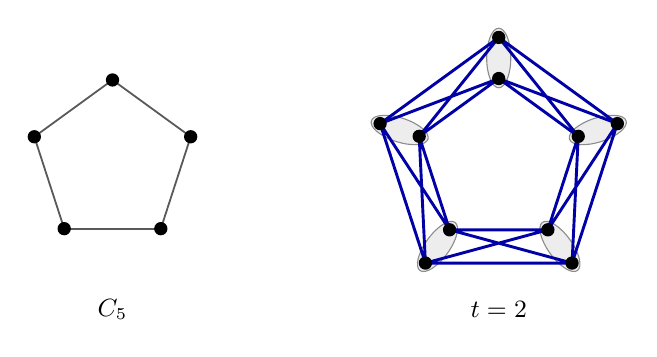
\begin{tikzpicture}[scale=0.9,every node/.style={font=\small}]
\foreach \i in {0,...,4}
  \coordinate (v\i) at ({90+72*\i}:1.16);
\foreach \i/\j in {0/1,1/2,2/3,3/4,4/0}
  \draw[unmarked edge] (v\i)--(v\j);
\foreach \i in {0,...,4}
  \node[graph vertex] at (v\i) {};
\node at (0,-2.08) {$C_5$};

\begin{scope}[xshift=5.45cm]
\foreach \i in {0,...,4}{
  \pgfmathsetmacro{\angle}{90+72*\i}
  \coordinate (a\i) at (\angle:1.18);
  \coordinate (b\i) at (\angle:1.76);
  \coordinate (part\i) at (\angle:1.47);
  \begin{scope}[shift={(part\i)},rotate=\angle]
    \draw[draw=black!45,fill=black!7] (0,0)
      ellipse[x radius=.42,y radius=.17];
  \end{scope}
}
\foreach \i/\j in {0/1,1/2,2/3,3/4,4/0}{
  \draw[marked edge] (a\i)--(a\j) (a\i)--(b\j)
    (b\i)--(a\j) (b\i)--(b\j);
}
\foreach \i in {0,...,4}{
  \node[graph vertex] at (a\i) {};
  \node[graph vertex] at (b\i) {};
}
\node at (0,-2.08) {$t=2$};
\end{scope}
\end{tikzpicture}
\caption{The cycle $C_5$ and its blow-up with two vertices per part.}
\label{fig:blowup}
\end{figure}

The proof is computer-assisted. We verify the flag inequalities used
in Sections~\ref{sec:uniform} and~\ref{sec:exact} by checking rational
certificates in exact arithmetic. For several small values of $\Delta$,
we derive necessary conditions for a strong clique to have more than
$f(\Delta)$ edges. In some cases, we enumerate the possible configurations
and verify that none can contain such a clique. In the other cases, we
encode the necessary conditions in Boolean formulas and verify that
none of these formulas has a satisfying assignment. The appendix describes
these checks. \textbf{Appendix~\ref{app:reproduction}} gives the commands
for reproducing them with the data, certificates and verification programs
in the repository~\cite{FGSTCode}.


\section{A Sketch of the Proof}\label{sec:overview}

We first use flag algebras to prove the bound $\frac{5}{4}\Delta(G)^2$
for $\omega(L(G)^2)$ in simple graphs. By counting parallel edges
with their multiplicities, we extend the bound to loopless multigraphs.
This settles the even-degree case.
For odd $\Delta=\Delta(G)\geq 9$, we show that if
$\omega(L(G)^2)>\Delta^2+\lfloor\frac{\Delta}{2}\rfloor^2$,
then $L(G)^2$ has a clique exceeding this bound whose vertices
correspond to a set of edges of $G$ that includes both a pair of
parallel edges and five edges forming an induced five-cycle in the
underlying simple graph of $G$. Counting around such cycles gives a
bound that contradicts the weighted flag inequalities. We handle the remaining small odd degrees separately,
thereby completing the proof.

\subsection{The Classical Flag Algebra Method}\label{subsec:flag-algebra}

Let $G$ be a graph. For a graph $H$ with $|V(H)|\leq |V(G)|$,
choose a subset $U\subseteq V(G)$ of size $|V(H)|$ uniformly at
random. The \emph{induced subgraph density} of $H$ in $G$ is the
probability that $G[U]$ is isomorphic to $H$. A \emph{type}
$\sigma$ is a graph with a distinct label on each vertex.
A \emph{$\sigma$-flag} is a partially labeled graph whose labeled
vertices induce $\sigma$ with the same labels. When the type
$\sigma$ is clear from the context, we call a $\sigma$-flag
simply a flag. Two flags are considered the same if there is an
isomorphism between them that preserves the labels. Fix a
labeled induced copy of $\sigma$ in $G$. For a $\sigma$-flag $F$
with $|V(F)|\leq |V(G)|$, choose uniformly at random a set of
$|V(F)|-|V(\sigma)|$ vertices outside this copy. The \emph{flag
density} of $F$ in $G$ is the probability that the chosen vertices
together with the fixed vertices induce a copy of $F$ with the
labels preserved. Fix a type $\sigma$. Let $\mathcal F^\sigma$
be the set of $\sigma$-flags, and let $\mathcal F^\sigma_n$ be
the set of $\sigma$-flags on $n$ vertices. Consider formal sums
$\sum_{J\in\mathcal F^\sigma}a_JJ$ with real coefficients, only
finitely many of which are nonzero. We add two such sums by
adding their coefficients at each flag $J$. Multiplication by
a scalar $\lambda$ sends each coefficient $a_J$ to $\lambda a_J$.
With these operations, it is easy to see that the formal sums
form a real vector space with basis $\mathcal F^\sigma$. We
denote this space by $\mathbb R\mathcal F^\sigma$.

For flags $F$ and $J$ with $|V(F)|\leq |V(J)|$, write $p(F;J)$
for the flag density of $F$ in $J$. We use $p(F;G)$ in the same
sense when the labeled copy of $\sigma$ in $G$ has been fixed.
For each flag $F$ and each
integer $n\geq |V(F)|$, form the vector
\[
  F-\sum_{J\in\mathcal F^\sigma_n}p(F;J)J.
\]
Let $\mathcal K^\sigma$ be the subspace of
$\mathbb R\mathcal F^\sigma$ spanned by these vectors as $F$
and $n$ vary. Put
$\mathcal A^\sigma=\mathbb R\mathcal F^\sigma/\mathcal K^\sigma$.
Two formal sums represent the same element of $\mathcal A^\sigma$
if their difference lies in $\mathcal K^\sigma$.

To define multiplication, let $F_1$ and $F_2$ be flags with
$r_1$ and $r_2$ unlabeled vertices, respectively. Put
$n=|V(\sigma)|+r_1+r_2$. For each $J\in\mathcal F^\sigma_n$,
choose $r_1$ of its unlabeled vertices uniformly at random
and put the remaining $r_2$ in the second group. Each group,
together with the labeled vertices of $J$, induces a flag.
Let $p(F_1,F_2;J)$ be the probability that the chosen group
gives $F_1$ and the remaining group gives $F_2$. The product
$F_1\cdot F_2$ is the element of $\mathcal A^\sigma$ represented by
\[
  \sum_{J\in\mathcal F^\sigma_n}p(F_1,F_2;J)J.
\]
To multiply two formal sums $\sum_i a_iF_i$ and $\sum_j b_jH_j$,
take the flag product $F_i\cdot H_j$ for each pair of terms, one
from each sum. Multiply each such product by the corresponding
coefficient $a_ib_j$ and add the results. Thus
\[
  \left(\sum_i a_iF_i\right)\cdot\left(\sum_j b_jH_j\right)
  =\sum_{i,j}a_ib_j(F_i\cdot H_j).
\]
Razborov showed that the product is well defined on the quotient
$\mathcal A^\sigma$~\cite{Razborov2007}. With this product,
$\mathcal A^\sigma$ is the \emph{flag algebra of type $\sigma$}.

Razborov's flag algebra method uses products of flag densities
to derive inequalities among induced subgraph
densities~\cite{Razborov2007,CarliSilvaOliveiraSato2016}.
Let $F_1$ and $F_2$ be $\sigma$-flags with $r_1$ and $r_2$
unlabeled vertices, respectively. Fix a labeled induced copy
of $\sigma$ in $G$, and suppose that the number of vertices
outside this copy is at least $\max\{1,r_1+r_2\}$. Choose
$r_1+r_2$ of these vertices uniformly at random. Together with
the labeled vertices, they induce a flag $J$. Choose $r_1$ of
the sampled vertices uniformly at random for the first group
and put the remaining $r_2$ in the second group. Given $J$,
the probability that the two groups, each taken together with
the labeled vertices, induce $F_1$ and $F_2$, respectively, is
$p(F_1,F_2;J)$. Since the probability of obtaining $J$ at the
first step is $p(J;G)$, the probability of obtaining both
$F_1$ and $F_2$ is
\[
  \sum_{J\in\mathcal F^\sigma_{|V(\sigma)|+r_1+r_2}}
  p(J;G)\,p(F_1,F_2;J).
\]
Now let $W$ be the set of vertices of $G$ outside the fixed labeled
copy of $\sigma$. Choose one of the $r_1$-element subsets of $W$
uniformly at random and call it $U_1$. Independently of this
choice, choose one of the $r_2$-element subsets of the same set
$W$ uniformly at random and call it $U_2$. Let $A$ be the event
that, for each $i\in\{1,2\}$, the subgraph induced by $U_i$ and
the labeled vertices gives the flag $F_i$. By independence,
$\Pr(A)=p(F_1;G)p(F_2;G)$.

Let $B$ be the event that $U_1\cap U_2=\varnothing$. By
independence and symmetry, conditional on $B$, all ordered
pairs $(S_1,S_2)$ of disjoint subsets of $W$ with $|S_1|=r_1$
and $|S_2|=r_2$ are equally likely. To count these pairs, choose
the union $S_1\cup S_2$ and then choose $S_1$ within it. There
are $\binom{|W|}{r_1+r_2}$ choices for the union and
$\binom{r_1+r_2}{r_1}$ choices for $S_1$ within each union.
Thus each pair has conditional probability
$\frac{1}{\binom{|W|}{r_1+r_2}\binom{r_1+r_2}{r_1}}$.

When the union is sampled first, each ordered pair $(S_1,S_2)$
of disjoint subsets of $W$ with $|S_1|=r_1$ and $|S_2|=r_2$
has probability
$\frac{1}{\binom{|W|}{r_1+r_2}\binom{r_1+r_2}{r_1}}$.
Under independent sampling, this is also the conditional
probability of $(U_1,U_2)=(S_1,S_2)$ given $B$. The two sampling
rules therefore give the same probability that the first set
and the second set, each together with the labeled vertices,
induce $F_1$ and $F_2$, respectively. For the experiment that
samples the union first, we computed this probability by
conditioning on the flag $J$ induced by the union and the
labeled vertices. Thus
\[
  \Pr(A\mid B)
  =\sum_{J\in\mathcal F^\sigma_{|V(\sigma)|+r_1+r_2}}
    p(J;G)\,p(F_1,F_2;J).
\]

It remains to compare $\Pr(A\mid B)$ with the probability $\Pr(A)$
under independent sampling. Since
$\Pr(A)=\Pr(A\mid B)\Pr(B)+\Pr(A\cap B^c)$, their difference is
bounded in absolute value by $\Pr(B^c)$. To bound $\Pr(B^c)$,
fix the outcome of $U_1$. The set $U_2$ is still a uniform
$r_2$-element subset of $W$, so each vertex of $U_1$ belongs
to $U_2$ with probability $\frac{r_2}{|W|}$. The event $B^c$
occurs if at least one of the $r_1$ vertices of $U_1$ belongs
to $U_2$. The union bound over the vertices of $U_1$ gives
$\Pr(B^c)\leq\frac{r_1r_2}{|W|}$, since the bound holds for every
choice of $U_1$. Since $\Pr(A)=p(F_1;G)p(F_2;G)$ and
$|W|=|V(G)|-|V(\sigma)|$, we have
\begin{equation}\label{eq:flag-product-estimate}
  \left|
    p(F_1;G)p(F_2;G)
    -\sum_{J\in\mathcal F^\sigma_{|V(\sigma)|+r_1+r_2}}
        p(F_1,F_2;J)p(J;G)
  \right|
  \leq \frac{r_1r_2}{|V(G)|-|V(\sigma)|}.
\end{equation}

Fix a list of $\sigma$-flags $F_1,\ldots,F_t$ and a real
symmetric positive semidefinite $t\times t$ matrix $Q=(Q_{ij})$.
For each $i$, let $r_i=|V(F_i)|-|V(\sigma)|$. Take $G$ large
enough for \eqref{eq:flag-product-estimate} to apply to every
pair $F_i,F_j$, and assume $|V(G)|\geq 2|V(\sigma)|$. Let
$\theta$ be an injective assignment of the labels of $\sigma$
to vertices of $G$ such that the assigned vertices, with
their labels, induce $\sigma$. Write $p_\theta(F;G)$ for
the density of a flag $F$ in $G$ with this assignment, and
let $v_\theta$ be the column vector with $i$th entry
$p_\theta(F_i;G)$. Since $Q$ is positive semidefinite,
\[
  0\leq v_\theta^{\mathsf T}Qv_\theta
    =\sum_{i,j=1}^{t}Q_{ij}\,
       p_\theta(F_i;G)p_\theta(F_j;G).
\]

For each pair $F_i,F_j$, expand the flag product $F_i\cdot F_j$
using flags on $|V(\sigma)|+r_i+r_j$ vertices, as in the definition
of multiplication. Multiply each expansion by $Q_{ij}$, add the
expansions, and collect terms to obtain the formal sum
$\sum_J c_JJ$. Thus the pair $F_i,F_j$ contributes
$Q_{ij}p(F_i,F_j;J)$ to $c_J$ when
$|V(J)|=|V(\sigma)|+r_i+r_j$. The coefficients $c_J$ depend only
on the fixed flags and $Q$.

By \eqref{eq:flag-product-estimate}, replacing
$p_\theta(F_i;G)p_\theta(F_j;G)$ by the expansion of
$F_i\cdot F_j$ with each flag replaced by its density in $G$
has error at most $\frac{r_ir_j}{|V(G)|-|V(\sigma)|}$.
Multiplying these bounds by $|Q_{ij}|$ and summing gives
\[
  \left|v_\theta^{\mathsf T}Qv_\theta
       -\sum_J c_Jp_\theta(J;G)\right|
  \leq
  \frac{\sum_{i,j=1}^{t}|Q_{ij}|r_ir_j}
       {|V(G)|-|V(\sigma)|}.
\]
Here and below, $J$ runs over the flags in the product
expansions. Since $|V(G)|\geq 2|V(\sigma)|$, the right-hand
side is at most $\frac{C}{|V(G)|}$, where
$C=2\sum_{i,j=1}^{t}|Q_{ij}|r_ir_j$. The nonnegativity of
$v_\theta^{\mathsf T}Qv_\theta$ now gives
\begin{equation}\label{eq:flag-density-lower-bound}
  \sum_J c_Jp_\theta(J;G)\geq-\frac{C}{|V(G)|}.
\end{equation}

Let $\Theta$ be the set of all injective assignments of the
labels of $\sigma$ to vertices of $G$. For each $\theta\in\Theta$
whose labeled vertices induce $\sigma$, use the densities
$p_\theta(J;G)$ defined above. For every other $\theta\in\Theta$,
put $p_\theta(J;G)=0$ for each $J$. The left-hand side of
\eqref{eq:flag-density-lower-bound} is then zero for those
assignments, so the inequality holds for every $\theta\in\Theta$.
Summing \eqref{eq:flag-density-lower-bound} over $\Theta$ and
dividing by $|\Theta|$ gives
\begin{equation}\label{eq:averaged-flag-density-lower-bound}
  \sum_J c_J
    \left(\frac{1}{|\Theta|}\sum_{\theta\in\Theta}p_\theta(J;G)\right)
  \geq -\frac{C}{|V(G)|}.
\end{equation}

Fix a flag $J$ in \eqref{eq:averaged-flag-density-lower-bound}, and
put $k=|V(J)|$, $s=|V(\sigma)|$ and $N=|V(G)|$. Choose
$\theta\in\Theta$ uniformly at random and then choose $k-s$ vertices
uniformly from the vertices that received no label. Let $S$ be
the union of the $k-s$ chosen vertices and the $s$ vertices
assigned labels by $\theta$. The two choices give $J$ if $G[S]$ with its assigned labels is
isomorphic to $J$. For a fixed $\theta$, the probability of
obtaining $J$ is $p_\theta(J;G)$. This also holds
under the zero convention when the labeled vertices do not
induce $\sigma$. When $\theta$ is chosen uniformly from $\Theta$,
the probability of obtaining $J$ in the two steps is
\[
  \frac{1}{|\Theta|}\sum_{\theta\in\Theta}p_\theta(J;G).
\]
We call this probability the \emph{average flag density} of $J$
in $G$.

For a fixed $k$-element set $S$ and a fixed injective assignment
$\theta$ of the labels within $S$, the probability of obtaining
the pair $(S,\theta)$ by assigning the labels first is
$\frac{1}{s!\binom{N}{s}\binom{N-s}{k-s}}$. Indeed, we must first
choose $\theta$ from the $s!\binom{N}{s}$ injective assignments
in $G$ and then choose the $k-s$ unlabeled vertices of $S$.
If we choose $S$ uniformly first and then choose an injective
assignment within $S$ uniformly, the probability of the same pair
is $\frac{1}{\binom{N}{k}s!\binom{k}{s}}$. These probabilities are
equal by the identity
$\binom{N}{s}\binom{N-s}{k-s}=\binom{N}{k}\binom{k}{s}$,
so the two sampling procedures give the same distribution.

Write $H_J$ for the unlabeled graph on the $k$ vertices of the
fixed flag $J$, with the same edges as $J$. For an unlabeled
graph $H$, write $p(H;G)$ for its induced subgraph density in $G$.
When $S$ is chosen first, the graph on which we assign labels is
the $k$-vertex induced subgraph $G[S]$ of the host $G$. A label
assignment within $S$ can give the flag $J$ only when
$G[S]\cong H_J$, an event of probability $p(H_J;G)$.
Choose an injective assignment of the labels of $\sigma$ to
vertices of $H_J$ uniformly at random. Let $q_\sigma(J)$ be the
probability that this assignment gives the flag $J$. Given a set
$S$ with $G[S]\cong H_J$, a uniform injective assignment of the
labels within $S$ gives $J$ with probability $q_\sigma(J)$. Hence
the average flag density of $J$ in $G$ satisfies
\[
  \frac{1}{|\Theta|}\sum_{\theta\in\Theta}p_\theta(J;G)
    =q_\sigma(J)p(H_J;G).
\]
Substituting this average into
\eqref{eq:averaged-flag-density-lower-bound} gives
\begin{equation}\label{eq:flag-unlabeled-lower-bound}
  \sum_J c_Jq_\sigma(J)p(H_J;G)
    \geq -\frac{C}{|V(G)|}.
\end{equation}

Inequality \eqref{eq:flag-unlabeled-lower-bound} gives a lower
bound on a linear combination of induced subgraph densities.
Flag algebra inequalities can be used to bound the induced
subgraph density of a fixed graph in a given graph class.
Let $d(G)$ be the density we want to bound and let $U$ be a
proposed upper bound. Suppose
identities for the graph class allow us to write $U-d(G)$ as
the left-hand side of \eqref{eq:flag-unlabeled-lower-bound}
plus a nonnegative linear combination of subgraph densities. Then
$U-d(G)\geq-\frac{C}{|V(G)|}$, or
$d(G)\leq U+\frac{C}{|V(G)|}$. The error tends to zero as
$|V(G)|$ grows. For example, when $d(G)$ is the edge density
in a triangle-free graph, the identity $p(K_3;G)=0$ can be
used in finding such an expression for $U-d(G)$.

\subsection{The Flag Algebra Method in Our Proof}\label{subsec:adapted-flags}

We adapt the local flag algebra method of Davey, Hurley, de Joannis de
Verclos, Kang and Volec~\cite{DaveyEtAlLocal2026,DaveyEtAlStrong2026},
who use the maximum degree to normalize counts of small graphs.
In our problem, we wish to express the size of a given strong clique
in terms of such counts. We mark the edges of the clique and record
both the marked and the unmarked edges, since an unmarked edge may
join two disjoint marked edges, as in \textbf{Figure~\ref{fig:marked-maps}}(a).

Suppose first that $G$ is simple, has maximum degree $\Delta$, and
contains a strong clique of $m>0$ edges. By
\textbf{Lemma~\ref{lem:regularization}}, we may take $G$ to be
$\Delta$-regular. The marked edges are the original $m$ clique edges.
A \emph{pattern} on the positions $0,\ldots,n-1$ assigns one of the
colors $0,1,2$ to each unordered pair of distinct positions.
A map from these positions to $V(G)$ determines a pattern. A pair
receives color $2$ if its images are joined by a marked edge, color
$1$ if they are joined by an unmarked edge, and color $0$ if they
coincide or are nonadjacent. For instance, in
\textbf{Figure~\ref{fig:marked-maps}}(b) the two positions $0$ and
$2$ have the same image.

\begin{figure}[htbp]
\centering
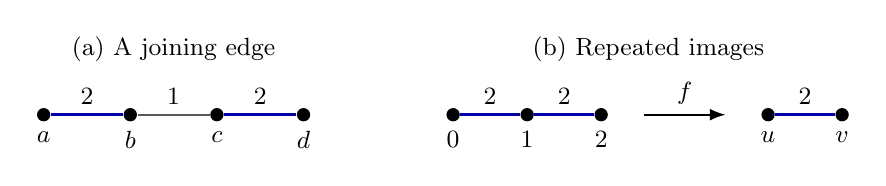
\begin{tikzpicture}[every node/.style={font=\small}]
\node at (1.65,0.83) {(a) A joining edge};
\node[graph vertex,label=below:$a$] (a) at (0,0) {};
\node[graph vertex,label=below:$b$] (b) at (1.1,0) {};
\node[graph vertex,label=below:$c$] (c) at (2.2,0) {};
\node[graph vertex,label=below:$d$] (d) at (3.3,0) {};
\draw[marked edge] (a)--node[above] {$2$} (b);
\draw[unmarked edge] (b)--node[above] {$1$} (c);
\draw[marked edge] (c)--node[above] {$2$} (d);

\begin{scope}[xshift=5.2cm]
\node at (2.48,0.83) {(b) Repeated images};
\node[graph vertex,label=below:$0$] (p0) at (0,0) {};
\node[graph vertex,label=below:$1$] (p1) at (0.94,0) {};
\node[graph vertex,label=below:$2$] (p2) at (1.88,0) {};
\node[graph vertex,label=below:$u$] (u) at (4,0) {};
\node[graph vertex,label=below:$v$] (v) at (4.94,0) {};
\draw[marked edge] (p0)--node[above] {$2$} (p1);
\draw[marked edge] (p1)--node[above] {$2$} (p2);
\draw[-{Latex[length=2mm]},semithick] (2.42,0)--node[above] {$f$} (3.46,0);
\draw[marked edge] (u)--node[above] {$2$} (v);
\end{scope}
\end{tikzpicture}
\caption{The edge $bc$ joins the marked edges in (a).
In (b), $f(0)=f(2)=u$ and $f(1)=v$.}
\label{fig:marked-maps}
\end{figure}

The graph underlying a pattern $F$ has an edge for each pair of
color $1$ or $2$. For the simple-graph calculation we use patterns
in which this graph is connected, the edges of color $2$ form a strong
clique in it, and the pair $\{0,1\}$ has color $2$. We call $(0,1)$
the ordered root. Let $h_F$ be the number of maps that give exactly
the colors of $F$. To see why we use the normalized count
$q_F=\frac{h_F}{2m\Delta^{n-2}}$, fix a spanning tree of the underlying
graph that contains the root edge. Choose the image of $(0,1)$
uniformly from the $2m$ ordered marked edges. Work outwards from the
root edge along the tree. Whenever the image of a position is known,
choose the image of each of its children independently and uniformly
from the $\Delta$ neighbors of that image. Each map counted by $h_F$
occurs with probability $\frac{1}{2m\Delta^{n-2}}$. Hence $q_F$ is the
probability that the sampled map gives the prescribed colors on
\emph{all} pairs of positions.

Fix such a pattern $T$ on $k$ positions. A flag $F$ of type $T$
is one of the patterns just described whose restriction to its first
$k$ positions is $T$. Given a map $f$ that gives the colors of $T$,
let $h_F(f)$ count the maps that give the colors of $F$ and agree
with $f$ on these $k$ positions. For a flag on $n$ positions, extend
a spanning tree of $T$ to a spanning tree of $F$. Starting with the
images fixed by $f$, sample the remaining $n-k$ images along the
tree. The probability of obtaining all the colors of $F$ is now
$\frac{h_F(f)}{\Delta^{n-k}}$. This plays the role of the flag
density for a fixed placement of the labels in
\textbf{Subsection~\ref{subsec:flag-algebra}}.

Take flags $F_i$ and $F_j$ of type $T$, with disjoint sets of positions
outside $T$. An extension of $f$ to $F_i$ and an extension of $f$ to
$F_j$ together define a map on the union of their positions. Its images
specify the colors of the remaining pairs, each with one position
in $F_i$ outside $T$ and one in $F_j$ outside $T$. Let
$\mathcal U_{ij}$ be the set of patterns on the union that agree with
both flags and in which the edges of color $2$ form a strong clique.
Every pair of extensions determines exactly one pattern in
$\mathcal U_{ij}$. Conversely, a map giving the colors of any
$H\in\mathcal U_{ij}$ and extending $f$ restricts to one extension
for each flag. Therefore
\[
 h_{F_i}(f)h_{F_j}(f)=\sum_{H\in\mathcal U_{ij}}h_H(f).
\]
The identity holds even when positions outside $T$ in the two flags
have the same image, since the map records their pair as color $0$.
Thus the formal sum $\sum_{H\in\mathcal U_{ij}}H$ in
\eqref{eq:colored-flag-product} gives an exact product rule for these
counts at every $\Delta$. Freedman, Lov\'asz and Schrijver use the
same multiplication of extension counts for partially labeled
graphs~\cite{FreedmanLovaszSchrijver2007}.

In \textbf{Figure~\ref{fig:flag-union}}, only the color of $\{2,3\}$
remains to be determined. Let $H_a$ be the pattern with color $a$
on that pair. All three choices are possible in the formal product.
When $a=2$, for example, the unmarked edge on $\{0,2\}$ joins the
two disjoint marked edges on $\{0,1\}$ and $\{2,3\}$. For these flags
the sum consists of $H_0,H_1,H_2$.

\begin{figure}[htbp]
\centering
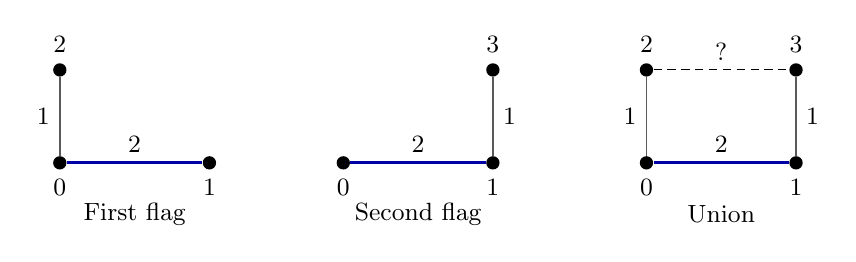
\begin{tikzpicture}[every node/.style={font=\small}]
\node[graph vertex,label=below:$0$] (a0) at (0,0) {};
\node[graph vertex,label=below:$1$] (a1) at (1.9,0) {};
\node[graph vertex,label=above:$2$] (a2) at (0,1.18) {};
\draw[marked edge] (a0)--node[above] {$2$} (a1);
\draw[unmarked edge] (a0)--node[left] {$1$} (a2);
\node at (0.95,-0.65) {First flag};

\begin{scope}[xshift=3.6cm]
\node[graph vertex,label=below:$0$] (b0) at (0,0) {};
\node[graph vertex,label=below:$1$] (b1) at (1.9,0) {};
\node[graph vertex,label=above:$3$] (b3) at (1.9,1.18) {};
\draw[marked edge] (b0)--node[above] {$2$} (b1);
\draw[unmarked edge] (b1)--node[right] {$1$} (b3);
\node at (0.95,-0.65) {Second flag};
\end{scope}

\begin{scope}[xshift=7.45cm]
\node[graph vertex,label=below:$0$] (c0) at (0,0) {};
\node[graph vertex,label=below:$1$] (c1) at (1.9,0) {};
\node[graph vertex,label=above:$2$] (c2) at (0,1.18) {};
\node[graph vertex,label=above:$3$] (c3) at (1.9,1.18) {};
\draw[marked edge] (c0)--node[above] {$2$} (c1);
\draw[unmarked edge] (c0)--node[left] {$1$} (c2);
\draw[unmarked edge] (c1)--node[right] {$1$} (c3);
\draw[densely dashed] (c2)--node[above] {$?$} (c3);
\node at (0.95,-0.65) {Union};
\end{scope}
\end{tikzpicture}
\caption{Two flags with common type on $\{0,1\}$. In their union,
the dashed pair has color $0$, $1$ or $2$. Undrawn pairs have color $0$.}
\label{fig:flag-union}
\end{figure}

The product rule gives inequalities as follows. Fix a list of flags of
type $T$. For the $i$th flag $F_i$, on $n_i$ positions, put
$v_i(f)=\frac{h_{F_i}(f)}{\Delta^{n_i-k}}$. Let $v(f)$ be the column
vector with these entries. The matrix
\[
 \frac{1}{2m\Delta^{k-2}}\sum_f v(f)v(f)^{\mathsf T}
\]
is positive semidefinite, since each summand is an outer product.
The sum ranges over the maps giving the colors of $T$. In its
$(i,j)$ entry the product rule sums the counts of patterns
$H\in\mathcal U_{ij}$ on $n_i+n_j-k$ positions. Each map counted by
$h_H$ has a unique restriction to $T$, so $\sum_f h_H(f)=h_H$.
The three factors in the denominator give
$2m\Delta^{k-2}\Delta^{n_i-k}\Delta^{n_j-k}
=2m\Delta^{n_i+n_j-k-2}$. Thus the entry is
$\sum_{H\in\mathcal U_{ij}}q_H$, as in \eqref{eq:moment-expansion}.
In the example of \textbf{Figure~\ref{fig:flag-union}} it is
$q_{H_0}+q_{H_1}+q_{H_2}$. Consequently each quadratic form of this matrix, evaluated at a fixed
real vector, gives a linear expression in the counts $q_H$ whose
value is nonnegative.

For a multigraph, a map into the simple support records which pairs
of vertices are adjacent. We also have to record how many edges of
the strong clique join each pair. Call an edge of the support
\emph{red} if at least one marked copy joins its endpoints. For each
red edge $uv$, distinguish one marked copy, called the \emph{base
copy}, and let $b_{uv}$ be the number of other marked copies, called
\emph{extra copies}. A pattern can now require an extra copy on one
or more specified edges. If the map sends such an edge to $uv$, there
are $b_{uv}$ choices for that copy. For a fixed map, multiplying
these numbers counts the choices on all specified edges.

For two flags with a common type, first choose the copies required
on the type. The choices on each flag outside the type are then
independent, so the same product rule counts pairs of extensions.
When the type itself requires extra copies, its map $f$ contributes
an outer product multiplied by the number of choices on the type.
This number is nonnegative, and the resulting matrix is again positive
semidefinite. \textbf{Subsection~\ref{sec:weighted-counts}} specifies
the weighted counts used in the multigraph proof.

\subsection{The Uniform Bound for Simple Graphs}\label{subsec:marked-edge-pairs}

We now express $\frac{m}{\Delta^2}$ in terms of the counts $q_F$.
Choose the images of $(0,1)$ and $(2,3)$ independently from the $2m$
ordered marked edges. The two choices may give the same edge. Each
choice determines the images of four positions and hence the colors of
all six pairs. If the two image edges are disjoint, a joining edge
exists because the marked edges form a strong clique. If they share
an endpoint, a position for that endpoint is adjacent in the pattern
to a position on the other edge. Thus the pattern is connected in
either case. Let $\mathcal B$ consist of the connected patterns on
these four positions whose edges of color $2$ form a strong clique
and include $\{0,1\}$ and $\{2,3\}$. Each choice of the two ordered
edges contributes to exactly one $h_F$ with $F\in\mathcal B$, and
every map counted by such an $h_F$ determines the two ordered edges.
Therefore
\[
 \sum_{F\in\mathcal B}h_F=(2m)^2,\qquad
 \frac{1}{2}\sum_{F\in\mathcal B}q_F=\frac{m}{\Delta^2}.
\]

To bound this sum we use the flag inequalities from
\textbf{Subsection~\ref{subsec:adapted-flags}} and the degree
equations. For the latter, fix a position in a pattern and require
one new position to map to a neighbor of its image. Every map of the
old positions has exactly $\Delta$ extensions. Sorting these
extensions by their pair colors gives \eqref{eq:degree-extension}
after normalization. The calculation in
\textbf{Subsection~\ref{sec:simple-proof}} uses the degree equations to
express $\frac{5}{4}-\frac{1}{2}\sum_{F\in\mathcal B}q_F$ as a sum
of nonnegative multiples of individual counts $q_F$ and of quadratic
forms of the positive semidefinite matrices with nonnegative weights. The identity is \eqref{eq:certificate-identity},
with rational coefficients checked in the proof of
\textbf{Lemma~\ref{prop:checked-certificate}}. Its right-hand side
is nonnegative. The identity for the two ordered edges now gives
$m\leq\frac{5}{4}\Delta^2$.

\subsection{From Simple Graphs to Multigraphs}\label{subsec:weighted-sketch}

Let $D$ be a positive integer and let $G$ be a loopless multigraph of
maximum degree at most $D$. Mark the $m>0$ edges of a strong clique.
Keep the subgraph induced by their endpoints. Between vertices joined
by marked edges, keep all the marked copies. Between any other two
adjacent vertices, keep one unmarked edge. Thus each pair of disjoint
marked edges still has a joining edge. Let $s$ be the number of red
edges in the simple support and $b=m-s$ the total number of extra
copies. The $s$ red edges form a strong clique in the simple support,
so the simple-graph bound gives $s\leq\frac{5}{4}D^2$.

The degree of a vertex in the reduced multigraph is its number of
distinct neighbors plus the number of extra copies incident with it.
As shown in \textbf{Subsection~\ref{sec:weighted-counts}}, we may add
unmarked edges and vertices to make the multigraph $D$-regular while
preserving its induced subgraph on the old vertices. Then, for each
vertex $v$, the extension by one incident edge has exactly $D$
choices. A neighbor $u$ joined to $v$ by an unmarked edge contributes
one choice. A neighbor on a red edge $uv$ contributes one choice of
the base copy and $b_{uv}$ choices of an extra copy. Counting these
choices in the weighted patterns gives the degree equations for
multigraphs.

Choose two ordered marked copies as in the simple-graph calculation.
There are $2s$ choices for an ordered base copy and $2b$ for an ordered
extra copy. Thus the numbers of choices using zero, one and two extra
copies are $(2s)^2$, $2(2s)(2b)$ and $(2b)^2$, respectively. Dividing
each count by $4mD^2$ gives the identity
\[
 \frac{s^2}{mD^2}+\frac{2sb}{mD^2}+\frac{b^2}{mD^2}
 =\frac{m}{D^2}.
\]
Each term on the left is a linear combination of the weighted
pattern counts. For example, in the last term each chosen edge of
the support contributes its number of extra copies.

Write $M=\frac{m}{D^2}$, $S=\frac{s}{D^2}$ and $e=\frac{b}{m}$.
Then $S=M(1-e)$. Suppose that $M>\frac{5}{4}$. The weighted flag
inequalities first give upper bounds on both $M$ and $e$. Degree
estimates on induced five-cycles of red edges, together with flag
inequalities in the simple support, give an upper bound on $S$.
The identity $e=1-\frac{S}{M}$ then gives a lower bound on $e$.
With $e$ restricted to this interval, the weighted flag inequalities
give a smaller upper bound on $M$. The successive bounds in the proof
of \textbf{Lemma~\ref{prop:multi-uniform}} yield $M<\frac{5}{4}$,
contradicting our assumption. This proves $m\leq\frac{5}{4}D^2$.
For even $D$, the right-hand side is $f(D)$.

\subsection{The Structure of a Counterexample}\label{subsec:odd-sketch}

Let $D=\Delta(G)$ be odd. If the bound $f(D)$ fails, mark exactly
$m=f(D)+1$ edges of a strong clique and keep the multigraph on their
endpoints as in \textbf{Subsection~\ref{subsec:weighted-sketch}}.
The definition of $f(D)$ gives
\[
 M=\frac{m}{D^2}=\frac{5}{4}-\frac{1}{2D}+\frac{5}{4D^2}.
\]
For $D\geq9$ this value is at least $\frac{98}{81}$, with equality
at $D=9$. If the simple support contained no induced five-cycle with
all five edges red, the flag inequality in~\cite[(G.2)]{FGSTSupplement} would give
$M<\frac{98}{81}$. Thus the support contains such a cycle, as stated
in \textbf{Lemma~\ref{lem:counterexample-cycle}}. We examine the degrees around
each such cycle to bound $s$, the number of distinct pairs of
endpoints of the $m$ marked edges.

Fix one of these cycles, say $c_0c_1c_2c_3c_4c_0$, and take
indices modulo five. For each $i$, let $U_i$ consist of the vertices
whose only neighbors on the cycle are $c_{i-1}$ and $c_{i+1}$ and
whose edges to both of these vertices are red. In particular,
$c_i\in U_i$. Take $x\in U_0$ and $y\in U_1$. The disjoint red edges
$xc_4$ and $yc_2$ must have a joining edge. The definitions of
$U_0,U_1$ exclude $xc_2$ and $yc_4$, and the induced cycle has no
edge $c_4c_2$. Thus $xy$ is an edge of the support. The same argument
with indices shifted shows that each vertex of $U_i$ is adjacent to
every vertex of $U_{i-1}$ and $U_{i+1}$.

In particular, $c_i$ is joined to at least $|U_{i-1}|+|U_{i+1}|$
distinct vertices in the multigraph. After counting one copy of each
of these edges, at most $D-|U_{i-1}|-|U_{i+1}|$ more edges can be
incident with $c_i$. The sum of these five upper bounds is
$R=5D-2\sum_{i=0}^4|U_i|$. For odd $D\geq11$, the degree count in
\textbf{Subsection~\ref{subsec:exact-large-degree}} shows that $R>\frac{D+1}{2}$ on
every such cycle in a counterexample.

To see how this structural restriction yields an inequality, let
$q_C$ be the number of ordered red induced five-cycles divided by
$2sD^3$. Here an ordered cycle has a specified starting vertex and
direction. Let $L_R$ be the sum of $\frac{R}{D}$ over the same
ordered cycles, divided by the same denominator. The bound on $R$
gives $L_R\geq\frac{q_C}{2}$. One of the flag inequalities for the
simple support in~\cite[(G.1)]{FGSTSupplement} gives
\[
 S+0.45119\left(L_R-\frac{q_C}{2}\right)\leq 1.221800627,
 \qquad\text{where }S=\frac{s}{D^2}.
\]
Its second term on the left is nonnegative. Thus
$S\leq1.221800627$. For odd $D\geq15$, the value of $M$ above
satisfies $M\geq\frac{11}{9}>1.221800627$. It follows that $s<m$,
so some pair of vertices is joined by at least two marked copies.
Moreover, $e=1-\frac{S}{M}$ gives an explicit lower bound on the
fraction of extra copies.

For $D=11,13$, the integer $R$ is odd, and the degree estimates
in \textbf{Subsection~\ref{subsec:exact-large-degree}} give $R\geq9$. Substituting
$L_R\geq\frac{9}{D}q_C$ into the flag inequalities gives $S<M$
in these two cases as well. At $D=9$, the finite simple-graph
bound excludes $s=m$. The remaining degree estimates restrict $e$
further. For each odd $D\geq9$ the weighted flag inequalities then
exclude the prescribed value $M=\frac{f(D)+1}{D^2}$ throughout the
allowed interval for $e$, as detailed in
\textbf{Table~\ref{tab:multi-odd}}. The cases $D=1,3,5,7$ are
settled separately in \textbf{Subsection~\ref{subsec:exact-small-degree}}. This proves
\textbf{Theorem~\ref{thm:multigraph}}.


\section{Comparison with Earlier Work}\label{sec:earlier-work}

\subsection{Earlier Work}

Let $H$ consist of the edges of a nonempty strong clique in $G$ and
their endpoints. Write $\Delta=\Delta(G)$ and $h=\Delta(H)$. Fix an
edge $xy$ of $H$. Every edge of $H$ meets $X=N_G(x)\cup N_G(y)$.
Indeed, $x,y\in X$, and any edge disjoint from $xy$ must have an
endpoint adjacent to $x$ or $y$. Thus $|E(H)|\leq |X|h\leq2\Delta h$.
Faudree, Gy\'arf\'as, Schelp and Tuza~\cite{FGST1990} asked what
would happen if this count came arbitrarily close to $2\Delta^2$.
The set $X$ would have close to $2\Delta$ vertices, and most of them
would have close to $\Delta$ edges of $H$ leading outside $X$, since
an edge inside $X$ is counted at both ends. Consider two such edges
$zu,z'u'$ with distinct $z,z'\in X$ and distinct $u,u'\notin X$.
If none of $zz',zu',z'u$ is present, then $uu'$ must be present.
The authors count these required edges at the outside neighbors of
a fixed $z$, together with the edges from those neighbors back to
$X$. The two counts exceed the available degree when
$|E(H)|>(2-\varepsilon)\Delta^2$ for sufficiently small absolute
$\varepsilon>0$. Hence $|E(H)|\leq(2-\varepsilon)\Delta^2$.

For simple graphs, \'{S}leszy\'{n}ska-Nowak~\cite{SleszynskaNowak2016}
used all the edges at a vertex $v$ with $d_H(v)=h$. At most $\Delta h$
edges of $H$ meet $N_G(v)$. Let $F$ consist of the remaining edges.
For every $a\in N_H(v)$, the set $N_G(a)\cap V(F)$ covers $E(F)$,
since each edge of $F$ must be joined to $va$ and neither endpoint is
adjacent to $v$. A vertex belonging to $j$ of these covers already
has $j$ neighbors outside $V(F)$ and hence has degree at most
$\Delta-j$ in $F$. When $h\geq\frac{3}{4}\Delta$, her count using
these covers gives $|E(F)|\leq\Delta^2-\frac{1}{2}\Delta h$.
Adding the edges meeting $N_G(v)$ gives
$|E(H)|\leq\Delta^2+\frac{1}{2}\Delta h\leq\frac{3}{2}\Delta^2$.
For smaller $h$, the bound $|E(H)|\leq2\Delta h$ already suffices.

Faron and Postle~\cite{FaronPostle2019} kept track of the degree sum
at the two ends of each edge of $H$. Write $\sigma=\sigma_G(H)$ for
the largest of these sums, with both degrees measured in $G$.
They chose $x$ of maximum degree in $H$ and, among its neighbors
in $H$, chose $y$ of largest degree in $H$. Their double counting
argument starts by summing the degrees in $H$ of the vertices in
$N_G(x)\cup N_G(y)$ and subtracting the edges counted twice.
For the second count, consider the edges from outside this union to
vertices adjacent to $x$ but not $y$, and those to vertices adjacent
to $y$ but not $x$. Each set forms a
smaller bipartite subgraph of $H$. In the first subgraph neither
endpoint of an edge is adjacent to $y$. For that edge to have a
joining edge to every edge of $H$ at $y$, each neighbor of $y$ in
$H$ must be adjacent to one of its endpoints. Those neighbors lie outside
the subgraph, so restricting $G$ to the vertices of this subgraph
lowers the endpoint degree sum by at least $d_H(y)$. The second
subgraph gives the corresponding decrease of at least $d_H(x)$.

Combining the two counts, Faron and Postle showed that an estimate
with coefficient $\beta\in[\frac{1}{4},\frac{1}{3}]$ for smaller
bipartite subgraphs of $H$ gives the estimate
$|E(H)|\leq\frac{1+\beta}{4}\sigma^2$ for general $H$.
Here the bipartite estimate is $|E(H')|\leq\beta\sigma_{G'}(H')^2$,
where $H'$ is the smaller bipartite subgraph and $G'=G[V(H')]$.
The edges of $H'$ still form a strong clique in $G'$ because all
their endpoints are retained. At $\beta=\frac{1}{3}$, the coefficient
$\frac{1+\beta}{4}$ is again $\frac{1}{3}$, so induction on $|E(H)|$
gives $|E(H)|\leq\frac{1}{3}\sigma^2\leq\frac{4}{3}\Delta^2$.

Kumar, Mohar and Pragada~\cite{KumarMoharPragada2026} improved the
bipartite estimate in this reduction. Suppose that $H$ is bipartite.
Choose $v$ with $d_H(v)=h$, put $A=N_H(v)$ and let
$B=V(H)\setminus N_G[v]$. For an edge $xy$ of $H[B]$, every
$a\in A$ must be adjacent to $x$ or $y$, since $va$ and $xy$ need
a joining edge. Thus $d_{G[B]}(x)+d_{G[B]}(y)\leq\sigma-h$,
and induction bounds $|E(H[B])|$ by $\beta(\sigma-h)^2$.
The same edges from $A$ to $B$ also enter the count at $A$.
Those outside $H$ use degree at $A$ without contributing to $|E(H)|$.
The authors subtract these edges when counting the edges of $H$
meeting $N_G[v]$. Combining this count with the induction bound
reduces the estimate to an inequality in $h/\sigma$, which they
verify for $\beta=\frac{620}{1987}$. The reduction above and
$\sigma\leq2\Delta$ then give
$|E(H)|\leq(1+\beta)\Delta^2=\frac{2607}{1987}\Delta^2$.

A different question is when a five-cycle must occur and what its
vertices tell us about the rest of the graph. Chung, Gy\'arf\'as,
Tuza and Trotter~\cite{CGTT1990} considered simple graphs in which
the entire edge set is a strong clique. After deleting isolated
vertices, such a graph has no induced subgraph consisting of two
disjoint edges. In the triangle-free, nonbipartite case, a shortest
odd cycle must have length five, since a longer induced cycle contains
two edges with no joining edge. Every vertex has exactly two neighbors
on the five-cycle. Vertices with the same two neighbors form one of
five independent sets. Every edge between successive sets is present,
so if their sizes in cyclic
order are $a_0,\ldots,a_4$, then the edge count is
$\sum_{i=0}^4 a_i a_{i+1}$ and $a_{i-1}+a_{i+1}\leq\Delta$ for
each $i$, with indices modulo five. Maximizing this sum gives
$f(\Delta)$. In the bipartite case each part contains a vertex
adjacent to the whole other part, so there are at most $\Delta^2$
edges. If there is a triangle, they find a maximum clique such that
every vertex outside it has a neighbor in it. Grouping the outside
vertices according to their neighbors in this clique and counting
the edges gives fewer than $f(\Delta)$ edges.

Cames van Batenburg, Kang and Pirot~\cite{CamesKangPirot2020}
allowed $H$ to be a proper submultigraph and assumed that $G$ has
no five-cycle. Again take $v$ with $d_H(v)=h$. Consider an edge
$xy$ of $H$ with both ends outside $N_G[v]$. Each $a\in N_H(v)$
must be adjacent to $x$ or $y$. If distinct $a,b\in N_H(v)$
were adjacent to $x$ and $y$, respectively, then $vaxybv$ would
be a five-cycle. Thus, when $|N_H(v)|\geq2$, one endpoint of $xy$
is adjacent to every vertex of $N_H(v)$. The authors count the
edges at these endpoints, then subtract the degree already used by
their neighbors in $N_H(v)$ when counting the remaining clique edges.
Together with the case $|N_H(v)|=1$, this gives
$|E(H)|\leq h(\sigma-h)\leq\frac{1}{4}\sigma^2\leq\Delta^2$.
Consequently a larger strong clique forces some five-cycle in $G$.
For our argument we need an induced five-cycle in the simple support
of $G$ with an edge of $H$ on each of its five pairs of endpoints.

\subsection{Highlights of the Proof}\label{subsec:method-highlights}

The main idea is to use the structure of a counterexample at odd
maximum degree to derive an inequality on edge multiplicities that
contradicts the weighted flag inequalities. Suppose that $G$ has odd
maximum degree $D$ and contains a strong clique of $m=f(D)+1$ marked edges.
For $D\geq9$, \textbf{Lemma~\ref{lem:counterexample-cycle}} gives an
induced five-cycle in the simple support of $G$. Each edge of the cycle
has the same endpoints as a marked edge of $G$. This allows us to
use the five sets suggested by the blow-ups of $C_5$ in the work
of Chung, Gy\'arf\'as, Tuza and Trotter~\cite{CGTT1990}, even when
the host has unmarked edges and parallel edges.

For each such cycle $C$, let $U_0,\ldots,U_4$ be the sets defined
in \textbf{Subsection~\ref{subsec:odd-sketch}}. All edges between
$U_i$ and $U_{i+1}$ are present in the simple support, with indices
taken modulo five. Thus at the $i$th cycle vertex at least
$|U_{i-1}|+|U_{i+1}|$ of its incident edges are already accounted for.
Summing over the five vertices leaves at most
$R(C)=5D-2\sum_{i=0}^4|U_i|$ further incidences.
When $D\geq11$, counting the marked edges in and outside these
sets shows that $R(C)\leq\frac{D+1}{2}$ would give $m\leq f(D)$.
Consequently $R(C)>\frac{D+1}{2}$ on every such cycle of a
counterexample. This use of restrictions on small induced subgraphs
to sharpen a flag bound is related to the stability arguments of
Pikhurko, Slia\v{c}an and Tyros~\cite{PikhurkoSliacanTyros2019}.

Let $s$ be the number of distinct pairs of vertices joined by
marked edges. Summing the lower bound on $R(C)$ over the cycles
and substituting it into the flag inequalities for the simple
support gives an upper bound on $s$. For example, for odd
$D\geq15$ we obtain
\[
  \frac{s}{D^2}\leq 1.221800627
  <\frac{11}{9}\leq\frac{m}{D^2}.
\]
Once one marked edge has been counted on each of the $s$ pairs,
the other $m-s$ marked edges are parallel copies. An upper bound
on $s$ is therefore a lower bound on the fraction $\frac{m-s}{m}$
of such copies. At $D=15$, for instance, the degree estimates give
$R(C)\geq11$ on every induced red five-cycle. Using this bound in the
inequalities for the simple support, and counting the extra copies at
their endpoints, gives $0.007\leq\frac{m-s}{m}\leq0.365$
in \textbf{Section~\ref{sec:exact}}.
With these restrictions, the weighted flag inequalities in the
$D=15$ row of \textbf{Table~\ref{tab:multi-odd}} give
$\frac{m}{D^2}<0.827$. Yet $m=f(15)+1=275$ requires
$\frac{m}{D^2}=\frac{11}{9}$. The other rows give the contradiction
for the remaining odd $D\geq9$.



\section{Auxiliary Lemmas}\label{sec:auxiliary}

We use a regular supergraph to count the ways to extend a map by one
vertex. We refine the regularization lemma of Davey et
al.~\cite{DaveyEtAlStrong2026} for simple graphs by extending it to
loopless multigraphs. The construction preserves the multiplicities
of the original edges and gives every new edge multiplicity one.

\begin{lemma}\label{lem:regularization}
Let $D\geq1$ be an integer and let $G$ be a finite loopless multigraph
with $\Delta(G)\leq D$. There is a finite $D$-regular loopless multigraph
$\widehat G$ containing $G$ as an induced subgraph such that every
edge of $\widehat G$ outside $G$ has multiplicity one. In particular, $\widehat G$ is simple
if $G$ is simple.
\end{lemma}

\begin{proof}
We must add $D-d_G(v)$ incidences at each vertex $v$. Their total
is $D|V(G)|-2|E(G)|$. If it is odd, then $D$ is odd, so adjoining one
isolated vertex makes the total even. Form a list containing $D-d(v)$
occurrences of each vertex $v$ of the resulting graph, where $d(v)$ is
its current degree. Partition the list into pairs. For a pair $(u,v)$,
take a new copy of $K_{D+1}$, delete an edge $xy$, and add the edges
$ux$ and $vy$. Use a different copy for each pair. This adds two
distinct edges even when $u=v$. Both $x$ and $y$ regain degree $D$,
and every occurrence in the list adds one incidence at the
corresponding vertex. Thus all degrees are $D$. Each added edge has
multiplicity one and at least one new endpoint, so the original
vertices induce $G$.
\end{proof}

A strong clique in $G$ is also a strong clique in $\widehat G$, since
every adjacency between endpoints of its edges is preserved. In the
counting arguments we mark only the edges of the chosen clique, so
all edges added in the construction are unmarked.

Vector inequalities are coordinatewise. For symmetric matrices $X$
and $Y$ of the same size, $\tr(XY)=\sum_{i,j}X_{ij}Y_{ij}$.

In the simple-graph calculation we will express the size of a strong
clique, divided by the square of the maximum degree, as a linear
function of the pattern counts. The calculation uses a system with $N=23{,}789$ coordinates, $3{,}516$ linear equations and
$57$ positive semidefinite matrix constraints. Write $Aq=b$ for the
linear equations and $o^{\mathsf T}q$ for the objective, where
$A\in\mathbb Q^{3516\times N}$, $b\in\mathbb Q^{3516}$ and
$o\in\mathbb Q^N$. For each $\ell\in[57]$, let
$K_\ell,D_{\ell1},\ldots,D_{\ell N}$ be symmetric rational matrices of
the same size. The $\ell$th matrix constraint is $M_\ell(q)\succeq0$,
where
\begin{equation}\label{eq:intro-affine-gram}
 M_\ell(q)=K_\ell+\sum_{j=1}^N q_jD_{\ell j}.
\end{equation}
The matrices and vectors are specified in~\cite[Section~A]{FGSTSupplement}.
For a symmetric matrix
$Q$ of the same size as $K_\ell$, define
$D_\ell^*(Q)\in\mathbb R^N$ by
\begin{equation}\label{eq:intro-trace-adjoint}
 (D_\ell^*(Q))_j=\tr(QD_{\ell j})\qquad(j\in[N]).
\end{equation}

\begin{lemma}\label{prop:certificate-principle}
Let $o\in\mathbb Q^N$ be an objective vector and
$\lambda\in\mathbb Q^{3516}$. For each $\ell\in[57]$, let $Q_\ell$
be a matrix of the same size as $K_\ell$ expressible as a finite
nonnegative rational linear combination of outer products
$ww^{\mathsf T}$ of rational vectors. Set
\begin{align}
 &r=A^{\mathsf T}\lambda-\sum_{\ell=1}^{57}D_\ell^*(Q_\ell)-o,
 \label{eq:residual}\\
 &C=b^{\mathsf T}\lambda+\sum_{\ell=1}^{57}\tr(Q_\ell K_\ell).
 \label{eq:dual-value}
\end{align}
We call $r$ the residual vector. If $r\geq0$, then every $q\in\mathbb R^N$ with $q\geq0$, $Aq=b$ and
$M_\ell(q)\succeq0$ for all $\ell\in[57]$ satisfies $o^{\mathsf T}q\leq C$.
If $q\in[0,1]^N$ satisfies the same equations and matrix constraints,
then $o^{\mathsf T}q\leq C-\sum_{j:r_j<0}r_j$, for any residual $r$.
\end{lemma}

\begin{proof}
By \eqref{eq:intro-affine-gram} and
\eqref{eq:intro-trace-adjoint}, each trace
$\tr(Q_\ell M_\ell(q))$ equals
$\tr(Q_\ell K_\ell)+D_\ell^*(Q_\ell)^{\mathsf T}q$.
Adding the scalar product of $r$ in \eqref{eq:residual} with $q$
cancels the terms involving $D_\ell^*(Q_\ell)$. Since $Aq=b$,
we have $\lambda^{\mathsf T}Aq=b^{\mathsf T}\lambda$, so
the definition of $C$ in \eqref{eq:dual-value} gives
\begin{equation}\label{eq:certificate-identity}
 C-o^{\mathsf T}q
 =\sum_{\ell=1}^{57}\tr\bigl(Q_\ell M_\ell(q)\bigr)
  +\sum_{j=1}^N r_jq_j.
\end{equation}
Write $Q_\ell=\sum_a\alpha_{\ell a}w_{\ell a}w_{\ell a}^{\mathsf T}$,
where each $\alpha_{\ell a}$ is nonnegative. Then
\[
 \tr\bigl(Q_\ell M_\ell(q)\bigr)=
 \sum_a\alpha_{\ell a}w_{\ell a}^{\mathsf T}M_\ell(q)w_{\ell a}\geq0
\]
because $M_\ell(q)$ is positive semidefinite. If $r\geq0$ and $q\geq0$,
the second sum in \eqref{eq:certificate-identity} is nonnegative.
For $0\leq q_j\leq1$, we have $r_jq_j\geq0$ if $r_j\geq0$ and
$r_jq_j\geq r_j$ if $r_j<0$. Thus the second sum is at least
$\sum_{j:r_j<0}r_j$ in that case.
\end{proof}

\section{Proof of the Bound \texorpdfstring{$\frac{5}{4}\Delta^2$}{5 Delta squared / 4}}\label{sec:uniform}

Let $G$ be a finite loopless multigraph with maximum degree $\Delta$.
We prove that $\omega(L(G)^2)\leq\frac{5}{4}\Delta^2$. We first
prove the bound for simple graphs. To extend it to multigraphs, we
count how many edges of a given strong clique join each pair of
adjacent vertices.

\subsection{The Bound \texorpdfstring{$\frac{5}{4}\Delta^2$}{5 Delta squared / 4} in Simple Graphs}
\label{sec:simple-proof}\label{sec:finite-model}\label{sec:identities}\label{sec:finite-instance}
\label{subsubsec:conditional-extension-counts}

By \textbf{Lemma~\ref{lem:regularization}}, a nonempty strong clique
in a simple graph of maximum degree $\Delta$ remains a strong clique
in a $\Delta$-regular simple graph. Let $G$ be this regular graph and
mark the set $S$ of edges in the given clique. We retain the other
edges of $G$, which may join the endpoints of disjoint marked edges.
The symmetric function
$c_G\colon V(G)\times V(G)\to\{0,1,2\}$ is given by
\[
 c_G(u,v)=
 \begin{cases}
  2,&uv\in S,\\
  1,&uv\in E(G)\setminus S,\\
  0,&u=v\text{ or }uv\notin E(G).
 \end{cases}
\]

\begin{defn}\label{def:patterns}
For an integer $n\geq2$, put $P_n=\{0,\ldots,n-1\}$. A \emph{pattern}
$F$ of order $n$ assigns a color $c_F(i,j)\in\{0,1,2\}$ to each pair
$ij=\{i,j\}$ of distinct positions in $P_n$, with $c_F(0,1)=2$. We
call $(0,1)$ the ordered root. The underlying graph $H$ of $F$ has
vertex set $P_n$ and edge set consisting of the pairs of color $1$
or $2$. We call $F$ \emph{connected} if $H$ is connected and
\emph{admissible} if the pairs of color $2$ form a clique in $L(H)^2$.
Equivalently, for every two disjoint pairs of color $2$, some pair
with one position in each has color $1$ or $2$.
Let $\mathcal F_n$ be the set of connected admissible patterns of order $n$.
\end{defn}

\begin{defn}\label{def:color-preserving-maps}
Let $F$ be a pattern of order $n$, and let $G$ be a finite simple graph
with marked set $S\subseteq E(G)$. A \emph{color-preserving map} from $F$
to $G$ is a map $f\colon P_n\to V(G)$ such that
$c_F(i,j)=c_G(f(i),f(j))$ for all distinct $i,j\in P_n$.
For fixed $G$ and $S$, let $h_F$ be the number of color-preserving maps
from $F$ to $G$.
\end{defn}

Distinct positions may map to the same vertex, in which case their
pair has color $0$.

\begin{lemma}\label{lem:pullback}
Let $G$ be a finite simple graph, let $S\subseteq E(G)$ be a clique
in $L(G)^2$, and let $n\geq 2$. Every map $f\colon P_n\to V(G)$ with
$c_G(f(0),f(1))=2$ gives an admissible pattern $F$ by setting
$c_F(i,j)=c_G(f(i),f(j))$ for all distinct $i,j\in P_n$.
\end{lemma}

\begin{proof}
Consider disjoint pairs $ij$ and $k\ell$ of color $2$ in $F$. Their
images are edges of $S$. If the image edges are disjoint, some
endpoint of one is adjacent to an endpoint of the other since $S$
is a clique in $L(G)^2$. The corresponding pair of positions has
color $1$ or $2$.

If the image edges have a common endpoint, we may name the positions
so that $f(i)=f(k)$. The pair $jk$ then maps to the marked edge
$f(j)f(i)$ and has color $2$. The same reasoning applies when the
image edges are equal.
\end{proof}

Let $G$ be a finite simple $\Delta$-regular graph with $\Delta>0$,
and let $S\subseteq E(G)$ be a nonempty clique in $L(G)^2$ of size $m$.
For $F\in\mathcal F_n$, define
\begin{equation}\label{eq:q-definition}
 q_F=\frac{h_F}{2m\Delta^{n-2}}.
\end{equation}
The factor $2m$ counts the possible images of the ordered root.
For the two-position pattern $E_\star$ with its unique pair marked,
we have $h_{E_\star}=2m$ and hence $q_{E_\star}=1$.

Two patterns $F,F'\in\mathcal F_n$ are equivalent if there is a
permutation $\pi$ of $P_n$ with
$c_F(i,j)=c_{F'}(\pi(i),\pi(j))$ for every pair $ij$ of distinct
positions. The preimage of $\{0,1\}$ under $\pi$ may be any pair of
color $2$ in $F$, with either ordering of its two positions. These
are isomorphism classes of the colored patterns with the root allowed
to move. We call them orbits, as in the data files.

For $k\geq2$, $F\in\mathcal F_k$ and $u\in P_k$, let
$\mathcal E(F,u)$ be the set of admissible patterns on $P_{k+1}$ whose
restriction to $P_k$ is $F$ and whose pair $uk$ has color $1$ or $2$.
Each such pattern is connected because its restriction to $P_k$ is
connected and the new position $k$ is adjacent to $u$.

\begin{lemma}\label{lem:coordinates}\label{lem:degree}
Suppose that $G$ is $\Delta$-regular and that its $m>0$ marked edges
form a strong clique. For every $k\geq2$ and $F\in\mathcal F_k$,
$q_F\in[0,1]$ and $q_{F'}=q_F$ for every $F'$ in the orbit of $F$.
For each $u\in P_k$,
\begin{equation}\label{eq:degree-extension}
 \sum_{F'\in\mathcal E(F,u)}q_{F'}=q_F.
\end{equation}
\end{lemma}

\begin{proof}
Since $F$ is connected, its underlying graph has a spanning tree
containing the root edge. Choose the image of the ordered root in
$2m$ ways. Then assign images to the remaining positions in order of
increasing distance from $\{0,1\}$ in the tree, so that each new
position has a tree neighbor whose image is already chosen. The pair
joining them has color $1$ or $2$, so the new image has at most
$\Delta$ choices. Thus $0\leq h_F\leq 2m\Delta^{n-2}$, and
$q_F\in[0,1]$ by \eqref{eq:q-definition}.

If $\pi$ is a permutation of $P_n$ with
$c_F(i,j)=c_{F'}(\pi(i),\pi(j))$ for all distinct $i,j$, then
$f\mapsto f\circ\pi$ maps the color-preserving maps of $F'$ to those
of $F$. Precomposing with $\pi^{-1}$ gives the inverse, so
$h_F=h_{F'}$. The two counts have the same denominator in
\eqref{eq:q-definition}, which gives $q_F=q_{F'}$.

Fix a color-preserving map $f$ of $F$. The image of $k$ can be any
of the $\Delta$ neighbors of $f(u)$, including neighbors already
used by $f$. Each choice determines the colors of all pairs involving
$k$ and therefore a unique extension pattern in $\mathcal E(F,u)$.
Admissibility follows from \textbf{Lemma~\ref{lem:pullback}}.
Conversely, a map counted by $h_{F'}$ for $F'\in\mathcal E(F,u)$
restricts to a color-preserving map of $F$ and sends $k$ to a neighbor
of the image of $u$. Thus
$\sum_{F'\in\mathcal E(F,u)}h_{F'}=\Delta h_F$.
Dividing by $2m\Delta^{k-1}$ gives \eqref{eq:degree-extension}.
\end{proof}

Index the $N=23{,}789$ relabeling orbits in
$\bigcup_{n=3}^6\mathcal F_n$ as in~\cite[Section~A.1]{FGSTSupplement}.
For each $j\in[N]$, set $q_j=q_F$ for any $F$ in orbit $j$.
We treat $q_{E_\star}=1$ as a constant. When we collect the terms of a
sum over labeled patterns by orbit, each labeled pattern contributes
once to its orbit coordinate.

The degree equations in $Aq=b$ are the identities in
\eqref{eq:degree-extension} written in the orbit coordinates.
In the row for $(F,u)$, each $F'\in\mathcal E(F,u)$ contributes
one to the column indexed by its orbit. If $F=E_\star$, the right
side of \eqref{eq:degree-extension} is $1$. Otherwise we subtract
one from the column indexed by the orbit of $F$ and set the right
side to $0$.

The pairs $(F,u)$ used for the degree equations are specified
in~\cite[Section~A.2]{FGSTSupplement}, with $F$ of order $2$, $3$,
$4$ or $5$. At order $5$, we use one pattern from each orbit and
take every position of that pattern in turn as $u$. The resulting
$3{,}516$ equations form the system
\begin{equation}\label{eq:linear-system}
 Aq=b.
\end{equation}
For example, the first row, for $F=E_\star$ and $u=1$, is
$q_1+q_2+q_3+2q_4+q_5=1$. The two extensions with color pairs
$(c_{F'}(0,2),c_{F'}(1,2))=(1,2)$ and $(2,1)$ contribute to
the same orbit, giving the coefficient of $q_4$.

A \emph{type} of order $k$ is a pattern $T\in\mathcal F_k$.
A \emph{flag of type $T$} is a pattern in $\mathcal F_n$, for some
$n\geq k$, whose restriction to $P_k$ is $T$. The positions of the
flag remain labeled when counting extensions. Let
$\mathcal L=(F_1,\ldots,F_s)$ be a list of flags of type $T$ of
orders $n_1,\ldots,n_s$, respectively. For a color-preserving map
$f$ of $T$ into $G$ and any flag $F$ of type $T$, let $h_F(f)$ be
the number of color-preserving maps from $F$ to $G$ that extend
$f$. For each $i\in[s]$, put $v_i(f)=\frac{h_{F_i}(f)}{\Delta^{n_i-k}}$.
Let $v(f)$ be the column vector with entries $v_i(f)$. Define the
\emph{moment matrix} for $T$ and $\mathcal L$ by
\begin{equation}\label{eq:moment-definition}
 M(T,\mathcal L)=\frac{1}{2m\Delta^{k-2}}
       \sum_{f:T\to G}v(f)v(f)^{\mathsf T}.
\end{equation}
The sum runs over all color-preserving maps of $T$ into $G$. If a
flag $F_i$ equals $T$, then $v_i(f)=1$ for each such map.

\begin{lemma}\label{lem:moment}
For any finite list $\mathcal L$ of flags of type $T\in\mathcal F_k$,
the moment matrix $M(T,\mathcal L)$ is positive semidefinite.
If $n_i+n_j-k\leq6$ for all $i,j\in[s]$, each entry is a nonnegative
integer linear combination of the coordinates of $q$ and the
constant $q_{E_\star}=1$.
\end{lemma}

\begin{proof}
By \eqref{eq:moment-definition}, for every $x\in\mathbb R^s$,
$x^{\mathsf T}M(T,\mathcal L)x$ is the sum of the squares
$(x^{\mathsf T}v(f))^2$ divided by $2m\Delta^{k-2}$, so it is
nonnegative.

To compute entry $(i,j)$, put $n=n_i+n_j-k$. In $P_n$, identify each position $r$ of $F_i$ with $r\in P_{n_i}$.
Identify position $r$ of $F_j$ with $r$ if $r<k$ and with $n_i+r-k$
otherwise. The flags agree on their intersection
$P_k$. The unspecified pairs have one position in
$P_{n_i}\setminus P_k$ and the other in $P_n\setminus P_{n_i}$.
Let $\mathcal U_{ij}$ be the set of admissible completions of the
colors of these pairs. Each completed pattern is connected because
the flags are connected and share the type. We write the product of
the two colored flags as the formal sum
\begin{equation}\label{eq:colored-flag-product}
 F_i\star_T F_j=\sum_{H\in\mathcal U_{ij}}H.
\end{equation}
The positions are labeled, so each admissible assignment of
the unspecified colors contributes one summand.

Fix a color-preserving map $f$ of $T$. A pair of extensions of $f$
to $F_i$ and $F_j$ gives a unique map on $P_n$, since the extensions
agree on $P_k$. The images of distinct positions may coincide,
including positions from different flags. Evaluating $c_G$ on the
images of each unspecified pair determines its color. The resulting
pattern belongs to $\mathcal U_{ij}$ by
\textbf{Lemma~\ref{lem:pullback}}. Conversely, a map counted by
$h_H(f)$ for $H\in\mathcal U_{ij}$ restricts to an extension of $f$
to each of the two flags. Counting these pairs and dividing by
$\Delta^{(n_i-k)+(n_j-k)}=\Delta^{n-k}$ gives
\begin{equation}\label{eq:colored-flag-evaluation}
 v_i(f)v_j(f)=\frac{\displaystyle\sum_{H\in\mathcal U_{ij}}h_H(f)}
                         {\Delta^{n-k}}.
\end{equation}
Thus the product in \eqref{eq:colored-flag-product} expresses the
product of the two normalized extension counts exactly.

Substitute \eqref{eq:colored-flag-evaluation} into
\eqref{eq:moment-definition}. Summing $h_H(f)$ over all maps
$f$ of $T$ gives $h_H$, since each color-preserving map of $H$
has a unique restriction to $T$. The total power of $\Delta$ in
the denominator is $(k-2)+(n-k)=n-2$. Hence
\eqref{eq:q-definition} gives
\begin{equation}\label{eq:moment-expansion}
 \bigl(M(T,\mathcal L)\bigr)_{ij}
 =\frac{\displaystyle\sum_{H\in\mathcal U_{ij}}h_H}{2m\Delta^{n-2}}
 =\sum_{H\in\mathcal U_{ij}}q_H.
\end{equation}
For the flags in \textbf{Figure~\ref{fig:flag-union}}, let $H_a$ be
the completion that assigns color $a$ to the pair $23$, for
$a\in\{0,1,2\}$. All three completions are admissible. In particular,
when $23$ has color $2$, the pairs $02$ and $13$ of color $1$ join
the marked pairs $01$ and $23$. The product in
\eqref{eq:colored-flag-product} is therefore $H_0+H_1+H_2$.
Both flags occur in the list of nine flags for the marked
two-position type in~\cite[Table~A.2]{FGSTSupplement}. Their product
gives the entry $q_{H_0}+q_{H_1}+q_{H_2}$ of the corresponding
moment matrix.

If $n=2$, the union is $E_\star$ and contributes the constant $1$.
If $3\leq n\leq6$, each summand contributes to the coordinate of
its relabeling orbit.
\end{proof}

In \eqref{eq:moment-expansion}, the coefficient of an orbit coordinate
counts the labeled completions in that orbit. If two flags differ
only by a permutation of their positions outside the type, that
permutation gives a bijection between their extensions of each
type map. We therefore use one representative of each class of
flags under permutations fixing the type positions.

The system uses $57$ pairs $(T_\ell,\mathcal L_\ell)$, with types of
order $2$, $3$ or $4$. The flag orders in
\cite[Table~A.2]{FGSTSupplement} ensure $n_i+n_j-k\leq6$ for every
pair of flags in the same list. For the graph counts, we set
$M_\ell(q)=M(T_\ell,\mathcal L_\ell)$. To write these matrices as in
\eqref{eq:intro-affine-gram}, let $(D_{\ell j})_{ab}$ count the labeled
completions in $\mathcal U_{ab}$ that belong to orbit $j$, where
$\mathcal U_{ab}$ is taken for the list $\mathcal L_\ell$.
A union of order $2$ occurs only when both flags equal the type
$E_\star$. This gives a $1$ at the first diagonal entry of $K_\ell$
in each of the two lists with this type, and every other entry of
every $K_\ell$ is $0$. By \textbf{Lemma~\ref{lem:moment}},
\begin{equation}\label{eq:positive-moments}
 M_\ell(q)\succeq0\qquad(\ell\in[57]).
\end{equation}

To express $\frac{m}{\Delta^2}$ in terms of $q$, we choose the
images of $(0,1)$ and $(2,3)$ independently from the $2m$ ordered
marked edges. Let $\mathcal B\subseteq\mathcal F_4$ consist of the
patterns in which both $01$ and $23$ have color $2$. For $j\in[N]$,
let $o_j$ be half the number of patterns in $\mathcal B$ belonging
to orbit $j$. Then
\begin{equation}\label{eq:objective-vector}
 o^{\mathsf T}q=\frac{1}{2}\sum_{F\in\mathcal B}q_F.
\end{equation}

\begin{lemma}\label{lem:finite-encoding}\label{lem:objective}
Let $G$ be a finite simple graph of maximum degree $\Delta>0$, and
let $S\subseteq E(G)$ be a strong clique of size $m>0$. For the system
specified in~\cite[Section~A]{FGSTSupplement}, there exists
$q\in[0,1]^N$ such that $Aq=b$, $M_\ell(q)\succeq0$ for all
$\ell\in[57]$, and
\begin{equation}\label{eq:objective-value}
 o^{\mathsf T}q=\frac{m}{\Delta^2}.
\end{equation}
\end{lemma}

\begin{proof}
Apply \textbf{Lemma~\ref{lem:regularization}} to $G$ with $D=\Delta$
and mark the $m$ edges of $S$ in the regular supergraph. Form $q$
from the counts in \eqref{eq:q-definition}. By
\textbf{Lemma~\ref{lem:coordinates}}, these counts lie in $[0,1]$
and depend only on their orbits. Equations \eqref{eq:linear-system}
and \eqref{eq:positive-moments} give $Aq=b$ and $M_\ell(q)\succeq0$
for all $\ell\in[57]$. It remains to evaluate $o^{\mathsf T}q$.

There are $(2m)^2$ choices for the two ordered marked images.
Each choice specifies a map of the four positions and therefore
an admissible pattern by \textbf{Lemma~\ref{lem:pullback}}.
Admissibility guarantees a pair of color $1$ or $2$ joining the
two marked pairs of positions. Thus the pattern is connected,
so the choice contributes to exactly one pattern in $\mathcal B$.
Conversely, a map counted by $h_F$ for $F\in\mathcal B$ sends both
pairs to ordered marked edges. Hence $\sum_{F\in\mathcal B}h_F=(2m)^2$.
Using this count in \eqref{eq:q-definition} and
\eqref{eq:objective-vector} gives
\[
 o^{\mathsf T}q
 =\frac{(2m)^2}{2\cdot2m\Delta^2}
 =\frac{m}{\Delta^2}.
\]
\end{proof}

It remains to bound the objective $o^{\mathsf T}q$. We give integer
coefficients for the bound in \textbf{Lemma~\ref{prop:certificate-principle}}
and verify them against the equations and flag products above.

The file \path{reproducibility/data/compact_certificate.json} stores
the vector $L\in\mathbb Z^{3516}$ of degree multiplier numerators.
For each block $\ell\in[57]$, it also gives a list of pairs
$(w_{\ell a},z_{\ell a})$ with $w_{\ell a}\in\mathbb Z_{\geq0}$ and
$z_{\ell a}\in\mathbb Z^{s_\ell}$, where $s_\ell$ is the number of
flags in $\mathcal L_\ell$. These pairs represent the weights
$\frac{w_{\ell a}}{24}$ and vectors $\frac{z_{\ell a}}{10{,}000}$
in a decomposition of $Q_\ell$. We use the common
denominator $\Lambda=24\cdot10{,}000^2=2{,}400{,}000{,}000$ and set
\begin{equation}\label{eq:integral-Q}
 B_\ell=\sum_a w_{\ell a}z_{\ell a}z_{\ell a}^{\mathsf T},
 \qquad Q_\ell=\frac{B_\ell}{\Lambda},
 \qquad \lambda=\frac{L}{\Lambda}.
\end{equation}
There are $4{,}110$ pairs with positive weight across the $57$ blocks.
The representation in \eqref{eq:integral-Q} shows that each $Q_\ell$
is positive semidefinite.

\begin{lemma}\label{prop:checked-certificate}\label{prop:quadratic-bound}\label{lem:rational-witness}
The numerators $L$ and $B_\ell$ in \eqref{eq:integral-Q} satisfy
\begin{align}
 &\rho=A^{\mathsf T}L-\sum_{\ell=1}^{57}D_\ell^*(B_\ell)
                  -\Lambda o\geq0,\label{eq:integer-residual}\\
 &b^{\mathsf T}L+\sum_{\ell=1}^{57}\tr(B_\ell K_\ell)
     =3{,}000{,}000{,}000=\frac{5}{4}\Lambda.
       \label{eq:integer-constant}
\end{align}
Consequently, every finite simple graph $G$ satisfies
$\omega(L(G)^2)\leq\frac{5}{4}\Delta(G)^2$.
\end{lemma}

\begin{proof}
The exact checks in~\cite[Section~B]{FGSTSupplement} verify the
degree and moment coefficients against \eqref{eq:degree-extension}
and \eqref{eq:moment-expansion}. With these coefficients, the
residual in \eqref{eq:integer-residual} has $23{,}590$ positive entries
and $199$ zero entries, and the constant in \eqref{eq:integer-constant}
is $3{,}000{,}000{,}000$. Thus $r=\frac{\rho}{\Lambda}\geq0$ and
$C=\frac{5}{4}$ for the multipliers in \eqref{eq:integral-Q}.
If $G$ has an edge, let $m$ be the size of a maximum clique in $L(G)^2$.
For the vector $q$ given by \textbf{Lemma~\ref{lem:finite-encoding}},
\textbf{Lemma~\ref{prop:certificate-principle}} now gives
$o^{\mathsf T}q\leq\frac{5}{4}$.
Since $o^{\mathsf T}q=\frac{m}{\Delta(G)^2}$ by \eqref{eq:objective-value},
we obtain $m\leq\frac{5}{4}\Delta(G)^2$.
If $G$ has no edges, the clique number is zero.
\end{proof}

We next record two consequences of the simple-graph count that we will
use in the proof for multigraphs. The first finds a marked induced
five-cycle when the clique is large enough. The second bounds the
degrees available around that cycle.

Let $G$ be a simple graph with maximum degree at most a positive
integer $D$, and let $m>0$ of its edges form a strong clique.
Mark these $m$ edges. Write $t=\frac{D}{2}$ and
$\mu=\frac{5}{4} D^2-m$. By \textbf{Lemma~\ref{prop:quadratic-bound}},
$\mu\geq0$. When $D$ is odd, $f(D)=5t^2-t+\frac{1}{4}$. A counterexample
with $m>f(D)$ therefore satisfies
\begin{equation}\label{eq:odd-counterexample}
 \mu\leq t-\frac{5}{4}.
\end{equation}

By \textbf{Lemma~\ref{lem:regularization}}, there is a $D$-regular
simple graph $\widehat G$ containing $G$ as an induced subgraph.
Only the original clique edges are marked. In particular every vertex
incident with a marked edge belongs to $G$.
\textbf{Lemma~\ref{lem:finite-encoding}} supplies the normalized
counts for $\widehat G$.

A marked induced five-cycle is an induced cycle of length five in
$\widehat G$ whose five edges are marked. Let $q_C$ be the normalized
count for the pattern with marked cycle $0,1,2,3,4,0$ and root $01$.
Every color-preserving map of this pattern is injective. Adjacent
positions have different images, and given two nonadjacent positions,
there is a third position adjacent to exactly one of them.
In the balanced blow-up with $b$ vertices in each part and all
edges marked, there are $10b^5$ such maps, from the ten cyclic
orderings and the choice of one vertex per part. Hence
$q_C=\frac{10b^5}{2(5b^2)(2b)^3}=\frac{1}{8}$ in that example.

Fix an ordered image $c_0,\ldots,c_4$ of the cycle, taking indices
modulo five. Let $U_i$ consist of the vertices whose neighbors on
the cycle are exactly $c_{i-1},c_{i+1}$ and whose edges to both
cycle vertices are marked. The sets $U_i$ are pairwise disjoint,
contain $c_i$ in $U_i$, and lie in $V(G)$ since every vertex in
them is incident with a marked edge.
\textbf{Figure~\ref{fig:odd-cycle-parts}} illustrates $U_0$. Define
\begin{equation}\label{eq:odd-core-defs}
 a_i=|U_i|,\qquad B=\bigcup_{i=0}^4 U_i,\qquad
 s_i=D-a_{i-1}-a_{i+1},\qquad R=\sum_{i=0}^4 s_i.
\end{equation}
By the definitions of the five sets, the neighbors of $c_i$ in $B$
are exactly $U_{i-1}\cup U_{i+1}$. Since $\widehat G$ is $D$-regular,
$s_i=|N_{\widehat G}(c_i)\setminus B|$. Summing over the five cycle
vertices gives $R=\sum_i|N_{\widehat G}(c_i)\setminus B|$, an upper
bound on the number of edges of $G$ from the cycle to $V(G)\setminus B$.

\begin{figure}[htbp]
\centering
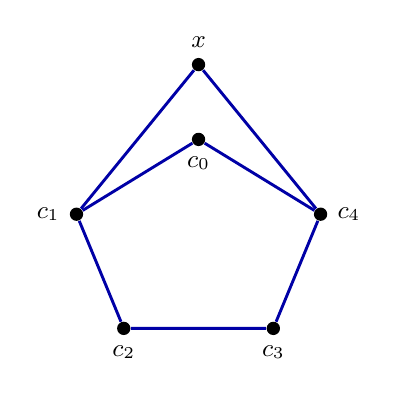
\begin{tikzpicture}[every node/.style={font=\small}]
  \node[graph vertex,label=below:$c_0$] (c0) at (0,1.4) {};
  \node[graph vertex,label=left:$c_1$] (c1) at (-1.55,0.45) {};
  \node[graph vertex,label=below:$c_2$] (c2) at (-0.95,-1) {};
  \node[graph vertex,label=below:$c_3$] (c3) at (0.95,-1) {};
  \node[graph vertex,label=right:$c_4$] (c4) at (1.55,0.45) {};
  \node[graph vertex,label=above:$x$] (x) at (0,2.35) {};
  \draw[marked edge] (c0)--(c1)--(c2)--(c3)--(c4)--(c0);
  \draw[marked edge] (c1)--(x)--(c4);
\end{tikzpicture}
\caption{A vertex $x$ in $U_0$ and its two marked edges to the cycle.}
\label{fig:odd-cycle-parts}
\end{figure}


To express $R$ in terms of the counts, let $L_R$ be the following
linear form in the six-position coordinates. The restriction to the
first five positions is the marked induced cycle. The coefficient
of a labeled extension is the number of neighbors of the sixth
position on the cycle if that position either has an unmarked edge
to the cycle or is adjacent to two consecutive cycle positions.
All other extensions have coefficient zero. A vertex outside $B$
with a cycle neighbor satisfies at least one of these two tests.
Indeed, if it fails both, it has at most two cycle neighbors and
all edges to them are marked. With only one such neighbor $c_i$,
its marked edge to $c_i$ has no endpoint in common with the
opposite cycle edge $c_{i+2}c_{i+3}$ and no edge joins their endpoints.
With two nonconsecutive marked neighbors, it belongs to one of
the sets $U_i$. Conversely, vertices of $B$ fail both tests.

Thus the sum over the sixth position is $R$ for each ordered
cycle. The denominators in \eqref{eq:q-definition} for five and
six positions differ by a factor of $D$. If $q_C>0$, this gives
$L_R=\frac{q_C}{D}\mathbb E[R]$, where the expectation is over a
uniformly chosen color-preserving map of the cycle pattern. If $q_C=0$,
there is no such map and $L_R=0$.

The five-cycle certificates give
\begin{equation}\label{eq:odd-moment-bounds}
 \frac{\mu}{D^2}\geq\gamma_C\Bigl(\frac{1}{8}-q_C\Bigr)-\epsilon_C,
 \qquad
 \frac{\mu}{D^2}\geq\gamma_R L_R-\epsilon_R.
\end{equation}
Both errors $\epsilon_C$ and $\epsilon_R$ are nonnegative. For the
first inequality we use either
$\gamma_C\geq\frac{99999}{100000}$ and $\epsilon_C\leq2\cdot10^{-9}$,
or $\gamma_C\geq\frac{6449}{10000}$ and $\epsilon_C\leq10^{-9}$.
For the second we use $\gamma_R\geq\frac{56425}{100000}$ and
$\epsilon_R\leq10^{-9}$. The files and checks are specified in
\cite[Sections~B and~C]{FGSTSupplement}.

Suppose that $\mu\leq\mu_*$, $\gamma_C\geq g_C>0$ and
$\gamma_R\geq g_R>0$. Put
$q_*=\frac{1}{8}-\frac{\mu_*+\epsilon_C D^2}{g_C D^2}$.
The first inequality in \eqref{eq:odd-moment-bounds} gives
$q_C\geq q_*$ when $q_C<\frac{1}{8}$, and the bound holds directly
when $q_C\geq\frac{1}{8}$ because $q_*\leq\frac{1}{8}$. If $q_*>0$,
using the second inequality and $L_R=\frac{q_C}{D}\mathbb E[R]$
gives a cycle with $R\leq\mathbb E[R]$ and hence
\begin{equation}\label{eq:odd-choose-anchor}
 R\leq\frac{\mu_*+\epsilon_R D^2}{g_R Dq_*}.
\end{equation}
Verified upper bounds on either error can be used in this estimate.

\begin{lemma}\label{lem:simple-cycle-counts}
For the sets defined in \eqref{eq:odd-core-defs}, every vertex of
$U_i$ is adjacent to every vertex of $U_{i+1}$. Moreover,
$|B|=\frac{5D-R}{2}$ and $a_i=\frac{D-R}{2}+s_{i-2}+s_{i+2}$ for every $i$.
\end{lemma}

\begin{proof}
For every $x\in U_i$ and $y\in U_{i+1}$ we have $xy\in E(G)$. The
marked edges $xc_{i-1}$ and $yc_{i+2}$ are disjoint. The
definitions of the parts exclude $xc_{i+2}$ and $yc_{i-1}$, and
$c_{i-1}c_{i+2}$ is excluded because the cycle is induced. Since
the marked edges form a clique in $L(G)^2$, we must have
$xy\in E(G)$. Thus a vertex of $U_i$ has at most $s_i$ neighbors
outside $U_{i-1}\cup U_{i+1}$.

The sum $A=\sum_i a_i s_i$ bounds the number of incidences at vertices
of $B$ after excluding the edges between $U_i$ and $U_{i+1}$ for all
$i$. Each remaining edge with both ends in $B$ contributes two
incidences. Put $e_0=\sum_i a_i a_{i+1}$, the number of edges between
parts $U_i$ and $U_{i+1}$.
Solving \eqref{eq:odd-core-defs} gives
\begin{equation}\label{eq:odd-core-sums}
 a_i=t-\frac{R}{2}+s_{i-2}+s_{i+2},\qquad
 |B|=\frac{5D-R}{2}.
\end{equation}
Summing the five equations for $s_i$ gives the formula for $|B|$.
For $a_i$, the two disjoint pairs of indices
$\{i-2,i+1\}$ and $\{i-1,i+2\}$ are the neighbor pairs of
$i+2$ and $i-2$, respectively. Subtracting their sizes from $|B|$
gives $a_i=|B|-2D+s_{i-2}+s_{i+2}$.
\end{proof}

By substituting \eqref{eq:odd-core-sums} into $\sum_i a_i s_i$
and using $2e_0=\sum_i a_i(D-s_i)$, we obtain
\begin{equation}\label{eq:odd-core-capacity}
 A=tR-\frac{R^2}{2}+2\sum_i s_i s_{i+2},
 \qquad
 e_0=5t^2-\frac{Rt+A}{2}.
\end{equation}
When $D$ is odd, $R=5D-2|B|$ is odd as well. To bound $\sum_i s_i s_{i+2}$,
consider the cycle on the indices with edges $i,i+2$. If two
nonadjacent vertices have positive weights, move their combined
weight onto the vertex with the higher sum of neighboring weights.
With the other weights fixed, the sum of products does not decrease.
Repeating leaves positive weights on a clique of size at most two.
The sum of products is then at most $\frac{R^2}{4}$. When $D$ is odd, integrality reduces this bound to $\frac{R^2-1}{4}$, so
\eqref{eq:odd-core-capacity} gives $A\leq tR-\frac{1}{2}$.

\begin{lemma}\label{lem:odd-unit-slack}
If an induced five-cycle with five marked edges has $R=1$, then $D$ is odd and $m\leq f(D)$.
\end{lemma}

\begin{proof}
Let $i$ be the unique index with $s_i=1$. Every vertex of the other
four parts has degree $D$ from the consecutive pairs alone. Thus a
marked edge outside the consecutive pairs has both ends in
$U_i\cup(V(G)\setminus B)$. The marked edge $c_{i+2}c_{i+3}$ has both
ends in parts whose consecutive neighbors are outside $U_i$. Both
vertices already have degree $D$ from those pairs, so neither is
an endpoint of, or adjacent to an endpoint of, the proposed marked
edge. This contradicts the clique property. Hence $m\leq e_0$.
For $R=1$, \eqref{eq:odd-core-capacity} gives
$A=t-\frac{1}{2}$ and $e_0=5t^2-t+\frac{1}{4}=f(D)$.
\end{proof}


\subsection{The Bound \texorpdfstring{$\frac{5}{4}\Delta^2$}{5 Delta squared / 4} in Multigraphs}
\label{sec:multigraph}\label{sec:weighted-counts}

The simple support of a multigraph records every adjacency that can
join two marked edges. To count the marked edges themselves, we must
also record how many copies have each pair of endpoints.

Let $D\geq1$ be an integer. Take a loopless multigraph $G$ with
$\Delta(G)\leq D$ and fix a
nonempty strong clique of size $m$ in $G$. Mark the edges of the clique
and restrict the host to the subgraph induced by their endpoints.
Every edge joining two disjoint marked edges has both endpoints in this
subgraph. Keep all marked edges. Between each pair of adjacent vertices joined
only by unmarked edges, keep one of those edges. The simple support $G_{\rm s}$ of the reduced
host therefore retains all adjacencies needed for the marked edges to
form a strong clique. Color an edge of $G_{\rm s}$ red if its endpoints are joined by a
marked edge of $G$, and blue otherwise. Let $s$ be the number of red
edges. For each red edge $uv$, choose one marked edge with endpoints
$u,v$ as its \emph{base copy}. Call the remaining marked edges with
these endpoints \emph{extra copies}. The red edges form a strong
clique in $G_{\rm s}$.

Put
\[
 b=m-s,\qquad M=\frac{m}{D^2},\qquad S=\frac{s}{D^2},
 \qquad e=\frac{b}{m}.
\]
Here $M$ and $S$ are normalized clique sizes and $e$ is the fraction
of marked edges that are extra copies. Thus $S=M(1-e)$. For each edge $uv$ of $G_{\rm s}$ let $b_{uv}$ be its
number of extra copies, with $b_{uv}=0$ for blue edges. Write
$d_{\rm s}(v)=d_{G_{\rm s}}(v)$ and
$j_v=\sum_{u\in N_{G_{\rm s}}(v)}b_{uv}$.
Then $\sum_v j_v=2b$ and $d_{\rm s}(v)+j_v\le D$.

We now write $G$ for this reduced multigraph. To obtain a
$D$-regular multigraph, apply \textbf{Lemma~\ref{lem:regularization}} and give each new edge
color blue. The reduced host is induced in the completion, and all
new edges have multiplicity one. Thus the red edges, their
multiplicities and the adjacencies among their endpoints are
unchanged. In the next counts we use the simple support of the
completed multigraph.

Use colors $0,1,2$ for a pair with equal or nonadjacent images,
a blue edge and a red edge, respectively. Let $P$ be a connected colored pattern on $n$ positions
with at least one red edge. As in \textbf{Definition~\ref{def:patterns}},
any two red edges in $P$ either meet or have endpoints joined by a red
or blue edge. In the weighted counts, $P$ has no designated root edge.
Let $T$ be a set of red edges of $P$ that form a forest on the positions.
Define
\[
 Q(P,T)=\frac{1}{2mD^{n-2}}
       \sum_{\phi}\ \prod_{uv\in T} b_{\phi(u)\phi(v)},
 \qquad
 X(P,T)=\frac{Q(P,T)}{|\operatorname{Aut}(P,T)|}.
\]
Here $\phi$ runs over color-preserving maps of the positions of $P$
to the simple support, and $\operatorname{Aut}(P,T)$ is the group of
permutations of the positions that preserve the pair colors and the
edge set $T$. As before, color $0$ permits equal images. Each edge
of $T$ contributes its extra multiplicity, even if two edges of $T$
have the same image, as in \textbf{Figure~\ref{fig:weighted-maps}}.
The forest condition is imposed on the positions. We use patterns
with $2\le n\le6$ and $|T|\le3$. Write $X$ for the vector of coordinates
$X(P,T)$, using one representative for each isomorphism class of pairs
$(P,T)$.

\begin{figure}[htbp]
\centering
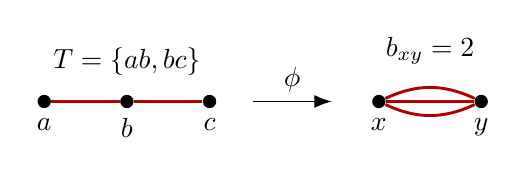
\begin{tikzpicture}[marked edge/.append style={draw=red!70!black}]
  \node[graph vertex,label=below:$a$] (a) at (0,0) {};
  \node[graph vertex,label=below:$b$] (b) at (1.05,0) {};
  \node[graph vertex,label=below:$c$] (c) at (2.1,0) {};
  \draw[marked edge] (a)--(b)--(c);
  \node[above=6pt] at (b) {$T=\{ab,bc\}$};
  \draw[-{Latex[length=2.2mm]}] (2.65,0)--node[above]{$\phi$}(3.65,0);
  \node[graph vertex,label=below:$x$] (x) at (4.25,0) {};
  \node[graph vertex,label=below:$y$] (y) at (5.55,0) {};
  \draw[marked edge] (x)--(y);
  \draw[marked edge] (x) to[bend left=25] (y);
  \draw[marked edge] (x) to[bend right=25] (y);
  \node[above=10pt] at (4.9,0) {$b_{xy}=2$};
\end{tikzpicture}
\caption{A weighted map with $\phi(a)=\phi(c)=x$ and $\phi(b)=y$.
Its weight is $b_{xy}^2=4$.}
\label{fig:weighted-maps}
\end{figure}


For the pattern $P$ consisting of a single red edge, summing over the
$2s$ oriented red edges of the simple support gives $Q(P,\varnothing)=1-e$. Summing their extra
multiplicities gives $Q(P,E(P))=e$, where $E(P)$ consists of the
single red pair. Each degree identity extends a fixed pattern
at a specified position. For a red extension, the unweighted and
weighted counts represent one base edge and the extra copies,
respectively. An extension to a blue neighbor counts its unique copy.
Together the blue and red extensions account for exactly
$D$ edge copies at the image of that position. The equations use
those extensions whose terms all occur in the model.

Choose two ordered marked edges independently, allowing the same
copy in both choices. Classify each choice as a base or an extra
copy. There are $(2s)^2$ ordered pairs of base copies,
$2(2s)(2b)$ ordered pairs with one base and one extra copy, and
$(2b)^2$ ordered pairs of extra copies. Each choice of the two
ordered copies determines the images of four positions in the
support. Their colors give a connected pattern because the two
edges belong to the strong clique. The forest weights count the
choices of an extra copy for each specified pair. As in
\eqref{eq:objective-vector}, divide the counts by $2mD^2$ and take
one half. The three contributions to the objective are
\[
 O_0=\frac{s^2}{mD^2},\qquad
 O_1=\frac{2sb}{mD^2},\qquad
 O_2=\frac{b^2}{mD^2}.
\]
Their sum is $M$ since $m=s+b$. More generally, adding an independent
ordered marked copy to a fixed pattern gives $2M Q(P,T)$
after normalization. Indeed, choosing the ordered copy multiplies the raw count by
$2m$, and the two new positions contribute a factor $D^2$ in the denominator. Replacing that copy by a base
or extra copy gives $2S Q(P,T)$ or $2Me Q(P,T)$. These formulas
give linear bounds when $M$, $S$ and $e$ are restricted to intervals.
For example, the bounds $e_-\le e\le e_+$ imply
\[
 O_2\le(e_-+e_+)\left(O_2+\frac{O_1}{2}\right)-e_-e_+M
\]
by expanding $M(e-e_-)(e_+-e)\ge0$.

Fix a type on $k$ positions and flags extending the type. In addition
to the colors, the type and flags specify forest edges as in $(P,T)$.
For a type map $\phi$, let $w(\phi)$ be the product of the extra
multiplicities on its specified forest edges. For the $i$th flag, on
$n_i$ positions, sum over the extensions of $\phi$ to that flag. Each
extension contributes the product of the extra multiplicities on its
specified forest edges outside the type. Let $v_i(\phi)$ be this sum
divided by $D^{n_i-k}$ and let $v(\phi)$ be the column vector with
entries $v_i(\phi)$. Then
\[
 \frac{1}{2mD^{k-2}}\sum_\phi w(\phi)v(\phi)v(\phi)^{\mathsf T}\succeq0.
\]
The matrix is a sum of outer products with nonnegative coefficients
because every extra multiplicity is a nonnegative integer. Its $(i,j)$ entry is a sum over pairs of extensions that agree on the type,
with denominator $2mD^{n_i+n_j-k-2}$. The two extensions may use the
same vertex outside the type. Group the pairs by the colors on the
remaining position pairs. Each resulting pattern uses the forest
edges in the type once, through $w(\phi)$. This writes each matrix
entry as a linear combination of coordinates $X(P,T)$. We use flag
lists for which these products lie in the specified pattern collection.
The same counting identity applies to the matrices formed from local
degrees and from counts of extensions satisfying degree constraints.

To bound $M$ we also need to count the edges at the vertices of an
induced red five-cycle in the reduced multigraph. Use the parts $U_i$
and remaining degrees $s_i$ from \eqref{eq:odd-core-defs} for the red
edges of its simple support. Call the vertices $c_0,\ldots,c_4$ of
the cycle its anchors, with indices modulo five, and put
$B=\bigcup_i U_i$. We call $B$ the core of this cycle.
Let $L$ be the number of blue pairs between $U_i$ and $U_{i+1}$,
summed over $i$. By \textbf{Lemma~\ref{lem:simple-cycle-counts}},
all pairs between these two parts are adjacent. Reserving one copy
for each such pair leaves at most $s_i$ incidences at each vertex of
$U_i$. Set $a_*=\frac{D-R}{2}$. Equations \eqref{eq:odd-core-sums}
and \eqref{eq:odd-core-capacity} applied to the simple support give
\begin{equation}\label{eq:multi-core-identities}
 a_i=a_*+s_{i-2}+s_{i+2},\qquad
 A=\sum_i a_is_i=\frac{RD}{2}-\frac{R^2}{2}
             +2\sum_i s_i s_{i+2}\le\frac{RD}{2}.
\end{equation}
In particular $R=5D-2|B|$ has the same parity as $D$.

We now bound the contribution of edges incident with vertices outside $B$.
Set $r=\frac{R}{D}$, $j=\frac{\sum_{i=0}^4j_{c_i}}{D}$,
$g=\frac{m}{D^2}-\frac{5}{4}$, and $\lambda=\frac{L}{D^2}$.

\begin{lemma}\label{lem:multigraph-cycle-counts}
If $g>0$, then $r>\frac{1}{2}$. For $\frac{1}{2}\le r\le1$,
\begin{equation}\label{eq:multi-joint}
 2g+2\lambda\le
 \frac{1+r}{2+r}\,r\left(r-\frac{1}{2}\right)
 -\frac{1+r^2}{2+r}\,j.
\end{equation}
\end{lemma}
\begin{proof}
The signature of a vertex $x$ is the set $\{i:xc_i\in E(G_{\rm s})\}$,
of size $k_x$. Summing the capacity $s_i$ at the five anchors gives
$K=\sum_{x\notin B}k_x\le R$. For $x\notin B$, let $h_x$ be its marked
degree, let $Q_x=|N_{G_{\rm s}}(x)\cap B|$, and let $b_x$ count its
blue pairs to $B$. For any marked edge $xy$, the union of the
signatures of $x$ and $y$ covers every edge of the cycle. In fact,
if $xy$ is disjoint from a cycle edge, the strong clique condition
gives an adjacency to one of the ends of that cycle edge. If $xy$
shares an endpoint with a cycle edge, its other cycle endpoint is
a neighbor of the shared vertex. Since a vertex cover of $C_5$ has
at least three vertices, a vertex with $k_x=0$ can have a marked
edge only to a vertex $y$ with $k_y\ge3$. In particular such an $x$
has no marked edge into $B$, since $k_y=2$ for $y\in B$.
A vertex outside $B$ of signature size two has at least one blue anchor pair. For
consecutive positions, a marked anchor pair would fail the strong
clique condition with the cycle edge opposite those positions. For
nonconsecutive positions, two marked anchor pairs would put the vertex
in $B$.

Every blue pair between consecutive classes uses two unmarked incidences
in $B$. The $b_x$ blue pairs of $x$ into $B$ use one unmarked incidence
in $B$ each, disjoint from the first set of incidences. The two
counts are illustrated in \textbf{Figure~\ref{fig:multigraph-cut}}.
Summing the marked incidences inside and outside $B$ gives
\begin{equation}\label{eq:multi-core-cut}
 2m\le D|B|-2L+\sum_{x\notin B}(h_x-b_x).
\end{equation}

\begin{figure}[htbp]
\centering
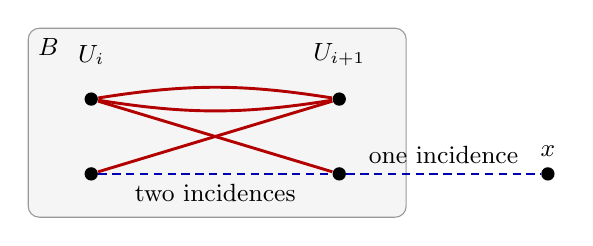
\begin{tikzpicture}[
  marked edge/.append style={draw=red!70!black},
  blue pair/.style={draw=blue!70!black,densely dashed,line width=0.95pt},
  font=\small
]
  \filldraw[fill=black!4,draw=black!40,rounded corners=4pt]
    (-0.65,-0.55) rectangle (4.15,1.85);
  \node[anchor=north west] at (-0.65,1.85) {$B$};
  \node at (0.15,1.51) {$U_i$};
  \node at (3.3,1.51) {$U_{i+1}$};
  \node[graph vertex] (a) at (0.15,0.95) {};
  \node[graph vertex] (b) at (0.15,0) {};
  \node[graph vertex] (c) at (3.3,0.95) {};
  \node[graph vertex] (d) at (3.3,0) {};
  \node[graph vertex,label=above:$x$] (x) at (5.95,0) {};
  \draw[marked edge] (a) to[bend left=9] (c);
  \draw[marked edge] (a) to[bend right=9] (c);
  \draw[marked edge] (a)--(d);
  \draw[marked edge] (b)--(c);
  \draw[blue pair] (b)--node[below] {two incidences} (d);
  \draw[blue pair] (d)--node[above] {one incidence} (x);
\end{tikzpicture}
\caption{A blue edge between consecutive parts contributes twice to
the degree sum on $B$. A blue edge from $x\notin B$ to $B$ contributes
once. Both copies of a marked pair contribute to marked degree.}
\label{fig:multigraph-cut}
\end{figure}


We first bound the total outside contribution after charging $b_x$ against
the core capacity. Suppose $k_x=1$ and $x$ has a marked edge to a vertex of $B$.
We show that $b_x\ge a_*+1$. Let $j$ be the sole index in the signature of $x$, and write $xy$ for
its marked edge with $y\in U_i$. Since $\{j,i-1,i+1\}$ covers the
cycle, $i=j\pm2$. Of the two cycle neighbors of $c_j$, let $c_k$
be the one nonadjacent to $y$. For each $u\in U_j$ the edge $c_ku$
is marked. Comparing it with $xy$ gives $xu$ or $yu$ in the support.
The edge $xy$ uses one of the $s_i$ extra incidences at $y$, so
$y$ has at most $s_i-1$ neighbors in $U_j$. At least
$a_j-s_i+1\ge a_*+1$ vertices of $U_j$ are therefore adjacent to
$x$. Each of these edges is blue, since $\{j,j-1,j+1\}$ does not
cover the cycle. If $xy$ is marked with $k_x=1$ and $k_y=2$, the union of their
signatures is a vertex cover of the cycle and hence has size three.
Whenever the union on an outside marked edge has size three, its two
omitted positions are nonconsecutive. Every red edge from either
omitted anchor into $B$ forces its other end to be adjacent to at least
one end of the outside marked edge. The core neighborhoods of those
ends therefore cover three classes. The other two classes have total
size at most $D$, so the three classes contain at least $|B|-D=D+a_*$
vertices. Each end uses one degree unit on the outside marked edge,
and so each sees at least $a_*+1$ vertices of $B$. If the end of
signature size one has no marked edge into $B$, these pairs are blue.

We redistribute the quantities $h_x-b_x$ over vertices outside $B$.
A vertex of signature size one with a marked core neighbor or a
marked neighbor of signature size two has $b_x\ge a_*+1$. Since
$h_x+b_x\le D$, it retains a contribution at most $R-2$. Any other
vertex of signature size one sends $\frac{1}{2}$ per marked copy to
its neighbors, all of which have signature size at least three. Its
remaining contribution is at most $\frac{D}{2}$. A vertex $x$ of
signature size zero with a marked neighbor of signature size three
has $b_x=Q_x\ge a_*$ by the comparison with the two omitted anchors.
It distributes its positive contribution uniformly over its marked
edges. Since $h_x\le D-Q_x$, the amount per copy is at most
$\frac{2R}{D+R}$. The other vertices of signature size zero use the
same rule, with at most one per copy and with recipients of
signature size at least four. We discard any negative contribution
left at a vertex of signature size zero.

A recipient of signature size three with a marked neighbor of
signature size zero also sees at least $a_*$ vertices of $B$, so it
has at most $\frac{D+R}{2}$ marked copies outside $B$. Multiplying
this bound by the larger of the two sending rates shows that it
receives at most $\max\{\frac{D+R}{4},R\}$. If it has no marked
neighbor of signature size zero, it receives at most $\frac{D}{2}$.
A recipient with at least four positions receives at most $D$.
Adding each recipient's own contribution, at most $D$, shows that
the total contribution at every outside vertex is at most
$k_x\max\{\frac{D}{2},R\}$ for $R\le D$. By \eqref{eq:multi-core-cut},
\begin{equation}\label{eq:multi-rough-discharge}
2m\le D|B|-2L+\max\left\{\frac{D}{2},R\right\}K.
\end{equation}

If $R\le \frac{D}{2}$, the right-hand side of \eqref{eq:multi-rough-discharge}
is at most $D|B|+\frac{D}{2}R=\frac{5}{2}D^2$.
Thus $g>0$ implies $r>\frac{1}{2}$.

Assume now that $\frac{1}{2}\le r\le1$. The $K$ adjacencies from the
five cycle vertices to the exterior and the $\sum_i j_{c_i}$ extra marked
incidences at those vertices use disjoint units of the remaining
degree $R$. Thus $K\le R-\sum_i j_{c_i}$.
Divide all vertex counts and degrees by $D$, and all
edge counts by $D^2$. Write $\eta=\frac{1-r}{2}$, $v=\frac{1+r}{2}$
and $\rho=\frac{2r}{1+r}$. An outside marked edge whose signatures
have union of size three has two ends each with normalized core
degree at least $\eta$. Each end has outside marked degree at most
$v$.

Let $x$ count the vertices of signature size one with a marked
neighbor in the core or a marked neighbor of signature size two.
Their total contribution in \eqref{eq:multi-core-cut}, in the
normalized units, is denoted by $C_1$. Each of these vertices has
at least $\eta$ blue pairs into the core, and $C_1\le rx$. Let
$p_2,p_3$ count the marked edges from these vertices to vertices of
signature size two and of signature size at least three, respectively.
Let $n_2$ count their neighbors of signature size two via a marked
edge. Also let $z_3,z_0$ count the vertices of signature size three
and of signature size zero, respectively, that meet a marked edge
joining these two groups. Denote the count of such edges by $p_{03}$.
The three groups counted by $n_2,z_3,z_0$ are disjoint. Each of their
vertices uses at least $\eta$ of the core capacity by the comparison
with the two omitted anchors, and $p_2\le v n_2$ and
$p_{03}\le v\min\{z_0,z_3\}$.

By \eqref{eq:multi-core-identities}, the total normalized capacity
of the core after reserving its consecutive pairs is at most
$\frac{r}{2}$. Deduct the core capacity used by the groups counted
by $x,n_2,z_3,z_0$. To bound $C_1$, add the exterior marked
counts $p_2+p_3$ and deduct the blue core pairs at the vertices
counted by $x$. This gives
$C_1\le\frac{r}{2}-2\eta x-\eta(n_2+z_3+z_0)+p_2+p_3$.
With $\theta=\frac{2r-1}{2+r}$ and $c=r-\theta=\frac{1+r^2}{2+r}$,
take weights $1-\theta,\theta$ on the two bounds for $C_1$ to get
\begin{equation}\label{eq:multi-joint-first}
 C_1\le cx+\frac{\theta r}{2}
     +\theta(p_2+p_3)-\theta\eta(n_2+z_3+z_0).
\end{equation}

For the other outside vertices, use the redistribution leading to
\eqref{eq:multi-rough-discharge}. A vertex of signature size two
retains at most one. Assign $\theta p_2-\theta\eta n_2$ in
\eqref{eq:multi-joint-first} to the group of such vertices. Since
$p_2\le v n_2$, its additional contribution is at most $\theta r$
per vertex, or at most $c=\frac{1}{2}+\frac{\theta r}{2}$ per signature
position after adding the original contribution.

For a vertex of signature size at least four, let $d_1$ be its
marked degree to the group counted by $x$. None of those edges
transfers any contribution to it, so its own and received
contributions sum to at most $2-d_1$. The corresponding bound for a
vertex of signature size three with no marked neighbor of signature
size zero is $\frac{3}{2}-\frac{d_1}{2}$. Adding the corresponding
$\theta d_1$ from $\theta p_3$ gives at most $c$ per signature
position in both cases, since $c\ge\frac{1}{2}$ and $\theta\le\frac{1}{3}$.

For the group counted by $z_3$, write $d_{1,3}$ for its marked
degree to the group counted by $x$. The vertices counted by $z_3$
have outside marked degree at most $v$ and receive at most
$\frac{1}{2}$ per marked copy, except for edges to the vertices
counted by $z_0$, which can transfer up to $\rho$ each. The total
after adding the corresponding terms of \eqref{eq:multi-joint-first}
is at most
\[
 \left(1+\frac{v}{2}\right)z_3
 -\left(\frac{1}{2}-\theta\right)d_{1,3}
 +\left(\rho-\frac{1}{2}\right)p_{03}-\theta\eta(z_3+z_0).
\]
Use $z_0\ge\frac{p_{03}}{v}$, then $p_{03}\le v z_3$, to
bound this by $(1+\rho v-2\theta\eta)z_3=3c z_3$. The second
substitution is valid because
$\rho-\frac{1}{2}-\frac{\theta\eta}{v}\ge0$ for $\frac{1}{2}\le r\le1$.
This accounts for all terms of \eqref{eq:multi-joint-first}.
The vertices of signature size one outside the group counted by
$x$ retain at most $\frac{1}{2}$ each. Thus the right side of
\eqref{eq:multi-core-cut}, divided by $D^2$, is at most
$\frac{5-r}{2}-2\lambda+c(r-j)+\frac{\theta r}{2}$.
Subtracting $\frac{5}{2}$ proves \eqref{eq:multi-joint}.

\end{proof}


Apply the simple-graph five-cycle counts to the red edges of
$G_{\rm s}$. Completing the simple support to a $D$-regular simple
graph adds only blue edges. All vertices of a red five-cycle and of
its five parts are incident with red edges. They therefore belong
to the old graph, which is induced in the completion. Thus the
completion preserves both the red five-cycles and their five
parts. Write $q_C$ for the number of ordered induced red five-cycles
divided by $2sD^3$ and $L_R$ for the sum of $\frac RD$ over these
cycles divided by the same quantity. If each such cycle satisfies
$R\geq\alpha D$, then summing this inequality gives $L_R\geq\alpha q_C$.

Applying the simple-graph certificate inequality to four choices
of objective gives
\begin{equation}\label{eq:support-projection-four}
\begin{aligned}
 S-0.99999q_C
   &\le \frac{5}{4}-\frac{0.99999}{8}+2\cdot10^{-9},\\
 S+0.5682L_R
   &\le \frac{5}{4}+10^{-9},\\
 S+0.4897(L_R-0.32q_C)
   &\le \frac{5}{4}-\frac{0.4897\cdot0.32}{8}+2\cdot10^{-9},\\
 S+0.45119\left(L_R-\frac{q_C}{2}\right)
   &\le \frac{5}{4}-\frac{0.45119}{16}+2\cdot10^{-9}.
\end{aligned}
\end{equation}
The coefficients and the error allowances in
\eqref{eq:support-projection-four} are rational.
\textbf{Appendix~\ref{app:multi-projection}} specifies the
four certificate checks. To see why the displayed coefficients
suffice, write each certified inequality as $S+\gamma Y\leq
\frac54+\varepsilon$, moving the multiple of $\frac18$ to the left.
For $Y\geq0$, replacing $\gamma$ by a smaller nonnegative coefficient
preserves the inequality. For $Y<0$ the bound follows from
$S\leq\frac54$.

For a given $\alpha>0$, substitute $L_R\geq\alpha q_C$ in
\eqref{eq:support-projection-four}. Each of the four inequalities
now has the form $S\leq a_i-b_iq_C$. Include $S\leq\frac54$ as
a fifth inequality, with $a_5=\frac54$ and $b_5=0$. Thus
\[
 S\leq S_{\max}(\alpha):=
 \max_{x\geq0}\min_{1\leq i\leq5}(a_i-b_ix),
 \qquad e\geq1-\frac{S_{\max}(\alpha)}{M}.
\]
The second line of \eqref{eq:support-projection-four} has
$b_2=0.5682\alpha>0$. The minimum of the five lines is continuous
and piecewise linear and tends to $-\infty$ as $x$ tends to infinity.
Its maximum is therefore attained at zero or at the nonnegative
intersection of two lines with different slopes. This gives a finite
rational calculation for $S_{\max}(\alpha)$.

These inequalities can also be imposed directly on $X$. Multiplying
each simple-graph inequality by $1-e=\frac{s}{m}$ changes the cycle
normalization from $2sD^3$ to $2mD^3$. Its term $(1-e)S$ is $O_0$,
and the same factor changes $L_R$ to the corresponding weighted
coordinate sum. All terms of the resulting inequality are linear
in the weighted counts.

Let $k\geq3$ and let $K$ be the vertex set of a red $K_k$ in the weighted host.
For each vertex $v$ put $a_v=|N_{G_{\rm s}}(v)\cap K|$ and let
$h_v$ and $d_{\rm blue}(v)$ count the marked and the unmarked edges
incident with $v$, respectively. Let $m_K$ count the marked edges with
both endpoints in $K$, with multiplicity, and put
$J_K=\sum_{v\in K}j_v$. For a marked edge $uv$, the set
$(N_{G_{\rm s}}(u)\cup N_{G_{\rm s}}(v))\cap K$ meets every edge
of the red clique. Indeed, a disjoint red edge in $K$ must have an
endpoint adjacent to $u$ or $v$, and the same holds when the red
edge shares an endpoint with $uv$. Every vertex cover of $K_k$ has
size at least $k-1$, so $a_u+a_v\geq k-1$. If $u\in K$, then
$a_u=k-1$ and $a_v\geq1$. If both endpoints lie in $K$, then
$a_u+a_v=2(k-1)$. Summing over all marked edges with multiplicity gives
\[
 (k-1)m+\sum_{v\in K}h_v+(k-3)m_K
 \le\sum_v a_vh_v
 \le D(kD-J_K)-\sum_{v\in K}d_{\rm blue}(v).
\]
For the upper bound, $\sum_v a_v=\sum_{v\in K}(D-j_v)=kD-J_K$
in the regular completion. Moreover, $a_vd_{\rm blue}(v)$ is at
least the number of blue neighbors of $v$ in $K$. Summing this
last inequality counts each blue incidence at $K$ and gives the
upper bound on $\sum_v a_vh_v$, since $h_v=D-d_{\rm blue}(v)$.
Using $\sum_{v\in K}(h_v+d_{\rm blue}(v))=kD$ now gives
\[
 (k-1)m\le kD(D-1)-DJ_K-(k-3)m_K.
\]
For $k=5$, the right side is at most $5D(D-1)-20$. Thus $4m\leq5D(D-1)-20$ if a red $K_5$ exists.
This is impossible when $m\geq\frac54D^2$. For odd $D$ it is also
impossible when $m=f(D)+1$, since then $4m=5D^2-2D+5$.
The coordinates of every pattern containing a red $K_5$ are
therefore zero in either case.

Fix a red edge $xy$. Let $U=N_{G_{\rm s}}(x)\setminus (N_{G_{\rm s}}(y)\cup\{y\})$
and let $W$ be the vertices adjacent to neither $x$ nor $y$. In the
host induced on $U\cup W$, mark only the previously marked edges
between $U$ and $W$. Edges within a part can still join endpoints of
these marked edges. For each marked edge $uv$ between $U$ and $W$, and
each red neighbor $z$ of $y$, the strong clique condition for $uv$
and $yz$ forces $uz$ or $vz$ to be a host edge. All such vertices $z$ lie
outside $U\cup W$, and different $z$ give different edges incident
with $u$ or $v$ that are absent from the induced host. Hence the Ore-degree $\sigma$ of the bipartite
marked subgraph in this induced host is at most $2D$ minus the
number of red neighbors of $y$.

If there is a marked edge between $U$ and $W$, the corresponding
upper bounds are
\[
 \frac{2973}{10000}\sigma^2\quad\text{for all copies},\qquad
 \frac{273323}{10^6}\sigma^2\quad\text{for base copies},\qquad
 \frac14\sigma^2\quad\text{for extra copies}.
\]
We give the counts that yield these bounds. In the induced host
let $H$ be the bipartite graph of marked edges between $U$ and $W$,
with their multiplicities. Suppose $H$ is nonempty, put $h=\Delta(H)$, and take
a vertex $v$ of marked degree $h$. Let $A=N_H(v)$,
$B'=V\setminus N[v]$ (where $V$ and $N[v]$ refer to the induced
host), $p=|A|$ and $\ell=\sigma-d(v)$, with $d(v)$ the degree in
the host. Every $a\in A$ has host degree at most $\ell$ since $va$
is marked. Let $T$ be the number of marked edges meeting $A$,
$P$ the number of unmarked edges from $A$ to $B'$, and
$F=H[B']$. Write $f=|E(F)|$ and $u=\Delta(F)$, with $u=0$ if
$F$ is edgeless. Every marked edge omitted by the counts $T$ and
$f$ has an endpoint in $N(v)\setminus A$. This set has at most
$d(v)-h$ vertices. Consequently
\[
 |E(H)|\leq h(\sigma-h)-h\ell+T+f,\qquad T+P\leq p\ell .
\]
For each $a\in A$, its neighbors in $B'$ meet every edge of $F$.
Since neither endpoint of that edge is adjacent to $v$, one must
be adjacent to $a$ to join the edge to $va$. Thus $f\leq u\ell$.
The same observation shows that the Ore-degree of the marked edges
in the host induced on $B'$ is at most $\sigma-p$. Indeed, for
each of the $p$ vertices of $A$, at least one edge to an endpoint
of the marked edge is lost when the host is restricted to $B'$.

First count all marked copies. On each pair joined by a marked
edge, remove the unmarked copies. On every other adjacent pair
retain one unmarked edge. This preserves all marked edges and all
adjacencies, and $\sigma$ still bounds the degree sum on each marked
edge. Use the counts above for this reduced host. Let $X'$ comprise the vertices of
$B'$ in the same part of $H$ as $v$. For $x\in X'$, let $h_x$
count the marked edges from $x$ to $A$, with multiplicity, and put
$f_x=d_F(x)$.
Each marked edge of $F$ has one endpoint in $X'$. For every
$a\in A$ it has an endpoint adjacent to $a$. The adjacency to $a$
either has an unmarked copy or is marked and meets the endpoint
in $X'$. Counting these possibilities yields
\[
 pf\leq uP+\sum_{x\in X'} h_xf_x .
\]
If $T,f>0$, let $\alpha=\frac{T}{T+f}$ and $\gamma=\frac{f}{T+f}$.
The identity
$(h_x+f_x)(\gamma^2h_x+\alpha^2 f_x)-h_x f_x
=(\gamma h_x-\alpha f_x)^2$ and the bound $h_x+f_x\leq h$
give $\sum_{x\in X'} h_xf_x\leq h(\gamma^2T+\alpha^2 f)
=\frac{hTf}{T+f}$. Substituting the resulting lower bound for
$P$ in $T+P\leq p\ell$ gives
\[
 |E(H)|\leq h(\sigma-h)+\left(1-\frac hp\right)T
       +\left(1-\frac hu\right)f
       +\frac{h^2Tf}{pu(T+f)} .
\]
If $f=0$, the previous counts give $|E(H)|\leq h(\sigma-h)$.
The induced host on $B'$ has fewer marked edges, since it omits
all marked edges at $v$. Applying bounds for this smaller graph with
Ore-degree at most $\sigma-p$ gives upper bounds for $f$.
The proof notes in the repository~\cite{FGSTCode} give further necessary
inequalities by comparing the marked neighborhoods in $A$ of
two vertices of $X'$. For example, if $x,x'\in X'$ are nonadjacent,
every vertex of $N_H(x)\cap A$ that is not adjacent to $x'$ must
be adjacent to every vertex of $N_H(x')\cap A$ that is not adjacent
to $x$. Otherwise two marked edges would have no edge joining their
endpoints. The rational interval check in \textbf{Appendix~\ref{app:ore-replay}}
uses these neighborhood inequalities and the bounds for the smaller
graph. It excludes $|E(H)|>\frac{2973}{10000}\sigma^2$ over the full
range of $\frac{h}{\sigma},\frac ph,\frac uh,\frac{T}{\sigma^2}$
and $\frac{f}{\sigma^2}$.

For the base copies, pass to the simple support, mark one edge on
each marked pair, and take the host induced on their endpoints.
This preserves every adjacency that joins two disjoint marked edges.
Let $s'$ be the number of marked edges in this simple host and let
$\sigma'\leq\sigma$ be their Ore-degree. Every vertex has a marked
neighbor, so its degree is at most $\sigma'-1$. For a connected
pattern $P$ on $k$ positions rooted at an ordered marked edge,
normalize its map count by $2s'(\sigma')^{k-2}$. The resulting
coordinate $q_P$ lies in $[0,1]$ by the spanning-tree bound and
vanishes if the marked edges of $P$ contain an odd cycle.
The count of two ordered marked edges in \eqref{eq:objective-value}
now gives the objective $\frac{s'}{(\sigma')^2}$.
The extension sum at one position is at most $q_P$. If $ij$ is a
marked edge of $P$, the two extension sums at $i$ and $j$ together
are at most $q_P$, since the sum of the two image degrees is at
most $\sigma'$. The moment matrices remain positive semidefinite
by \textbf{Lemma~\ref{lem:moment}}. The rational certificate in
\textbf{Appendix~\ref{app:ore-replay}} combines the extension inequalities
with nonnegative multipliers and the moment matrices with
positive semidefinite matrices. Each negative residual coefficient
is charged its absolute value, using $0\leq q_P\leq1$. The resulting
upper bound on $\frac{s'}{(\sigma')^2}$ is
$\frac{27332270490572378277}{10^{20}}<\frac{273323}{10^6}$.
This proves the asserted bound for base copies.

Finally, mark only the extra copies between $U$ and $W$, reserving
one base copy on each originally marked pair as an unmarked edge.
Every adjacent pair of vertices now has an unmarked edge joining it.
Apply the same counts with $H$ the graph of these extra copies.
The result is immediate if $H$ is empty. Otherwise, for
every pair consisting of $a\in A$ and an edge of $F$, the
joining adjacency has an unmarked copy, and each such copy serves
at most $u$ edges of $F$. Therefore $pf\leq uP$.
If $f=0$, the first two inequalities give $|E(H)|\leq
h(\sigma-h)$ because $p\leq h$. If $f>0$, then $u>0$, and
\[
 |E(H)|\leq h(\sigma-h)-(h-p)\ell+
          \left(1-\frac pu\right)f
 \leq h(\sigma-h)+\left(1-\frac hu\right)f
 \leq h(\sigma-h).
\]
Here the second inequality uses $f\leq u\ell$ and $p\leq h$,
and the last uses $u\leq h$. Finally $h(\sigma-h)\leq
\frac{\sigma^2}{4}$.

Multiplying any of the three bounds by the nonnegative forest
weight of the root and summing over root maps gives a linear
inequality for $X$. Expanding a neighbor count uses one further
position, and expanding its square or counting another edge uses
two.

Write $AX=(1,0,\ldots,0)^{\mathsf T}$ for the degree and sampling
equations, $NX\le0$ for the linear inequalities, and $G_i(X)\succeq0$
for the matrix inequalities. To bound $M$, take a vector
$\lambda$ with first entry $\lambda_0$, a nonnegative vector $\rho$, and matrices $P_i$
given as nonnegative sums of rational rank-one outer products.
Let $G_i^*$ be the adjoint defined by
$(G_i^*(P_i))^{\mathsf T}X=\tr(P_iG_i(X))$. The constraints give $\rho^{\mathsf T}NX\leq0$ and
$\tr(P_iG_i(X))\geq0$. Thus, for every feasible $X$,
\[
 \left(A^{\mathsf T}\lambda+N^{\mathsf T}\rho
        -\sum_iG_i^*(P_i)\right)^{\mathsf T}X
 \le\lambda_0 .
\]
Let $r$ be the coefficient vector on the left minus the coefficient
vector of $M$. If $0\le X_j\le U_j$ for each coordinate $j$, then
$M\le\lambda_0+\sum_{j:r_j<0}(-r_j)U_j$. For a coordinate $X(P,T)$,
an upper bound is
$\frac{1-e}{|\operatorname{Aut}(P,T)|}$ for $T=\varnothing$ and
$\frac{e}{|\operatorname{Aut}(P,T)|}$ otherwise. To obtain it, start at
a red edge, in $T$ if $T$ is nonempty, and extend along a
spanning tree containing $T$. Each new position contributes at
most $D$ in support count or extra multiplicity. The certificates
also use bounds on sums of coordinates of equal order and
equal forest size, obtained by counting all labeled spanning
trees containing the specified red root. Positive residuals
can be dropped since the coordinates are nonnegative. With these bounds the total correction is affine in $e$, so
its maximum over the allowed interval is attained at an endpoint. For an infeasibility certificate, the objective
is zero and the compensated right side is negative.


\begin{lemma}\label{prop:multi-uniform}
Every strong clique of size $m$ in a finite loopless multigraph of maximum
degree at most $D$ satisfies $m\le\frac{5D^2}{4}$. If $m>0$, $D>0$, and
$M\ge\frac{4967}{4000}$,
then $e<\frac{1}{4}$.
\end{lemma}

\begin{proof}
If $m=0$ the asserted bound holds. Otherwise $D>0$, and the
red edges form a strong clique of size $s$ in the simple support,
which has maximum degree at most $D$. Thus
\textbf{Lemma~\ref{prop:quadratic-bound}} gives $S\leq\frac{5}{4}$.
The five-position certificates in~\cite[Section~G.4]{FGSTSupplement}
exclude $M\geq\frac{4967}{4000}$ and $e\geq\frac14$ simultaneously,
giving the second assertion. They also give
$e<\frac{421}{2000}$ for $M\geq\frac54$ and $M<1.28492$ for
$M>\frac54$.

Suppose that $M>\frac54$. For an induced red five-cycle put
$r=\frac RD$ and $g=M-\frac54$. The degree estimates in
\textbf{Lemma~\ref{lem:multigraph-cycle-counts}} give $r>\frac12$.
When $r\leq1$, \eqref{eq:multi-rough-discharge} implies
$2g\leq r(r-\frac12)$, and \eqref{eq:multi-joint} gives the
stronger inequality
\[
 2g\leq\frac{1+r}{2+r}r\left(r-\frac12\right).
\]
Both right-hand sides are increasing on $[\frac12,1]$.
For a proposed lower bound $M_-$ on $M$, substitute
$g\geq M_--\frac54$ and solve for a lower bound $\alpha$ on $r$.
For example, if $M_-=1.283$, then
$0.6084(0.6084-\frac12)<2(1.283-\frac54)$, so $r>0.6084$.
All values of $\alpha$ in \textbf{Table~\ref{tab:uniform-chain}}
are at most one and hence also apply when $r>1$.
It follows from \eqref{eq:support-projection-four} that
$e\geq1-\frac{S_{\max}(\alpha)}{M_-}$. This argument includes the
case of no induced red five-cycle, when $L_R=q_C=0$.

\begin{table}[htbp]
\centering
\caption{Intervals excluded by the six-position certificates. Each row
gives a certified upper bound for $M$ strictly below $M_-$.}
\label{tab:uniform-chain}
\begin{tabular}{@{}rrrr@{}}
\toprule
$M_-$ & $M_+$ & $\alpha$ & Lower bound on $e$\\
\midrule
1.283 & 1.28492 & 0.6084 & 0.051\\
1.279 & 1.283 & 0.6446 & 0.049\\
1.274 & 1.279 & 0.6242 & 0.0445\\
1.268 & 1.274 & 0.5978 & 0.0395\\
$\frac54$ & 1.274 & 0.5 & 0.0225\\
\bottomrule
\end{tabular}
\end{table}

For each row, assume $M_-\leq M\leq M_+$. On this interval the
weighted counts satisfy the lower bound on $e$ in the last column
and $e<\frac{421}{2000}$. The rational certificates for these
intervals, including the corrections for negative residuals, are
specified in~\cite[Section~G.4]{FGSTSupplement}. The first three
rows successively exclude $M\geq1.283$, $M\geq1.279$ and
$M\geq1.274$. The last row now applies throughout the remaining
interval and gives
\[
 M\leq\frac{124968062205915704703985647}
                 {100000000000000000000000000}<\frac54,
\]
contrary to $M>\frac54$.
\end{proof}

The quadratic bound gives $m\leq f(D)$ for even $D$. For odd $D$
we shall need one further estimate on the number of extra copies.

\begin{lemma}\label{lem:multi-extra}
Suppose $b>0$ and set $A=\frac{\sum_v j_v^2}{2bD}$. Then
\[
 M\le 2-\left(2+\frac{1}{D}\right)A-\frac{1}{D^2},
 \qquad
 Me\le 2A(1-A)-\frac{A}{D}.
\]
In particular, $e\le 1-\frac{M}{2}$ whenever $M\ge1$.
\end{lemma}

\begin{proof}
Count ordered pairs $(g_1,g_2)$ of marked edges, allowing $g_1=g_2$.
For each ordered pair of marked edges, the strong clique property gives adjacent vertices
$u,v$ with $u$ an endpoint of $g_1$ and $v$ an endpoint of $g_2$.
If the edges share an endpoint, there are at least two
such ordered pairs $(u,v)$. Among the $b^2$ ordered pairs of extra copies,
exactly $\sum_v j_v^2-\sum_{uv\in E(G_{\rm s})}b_{uv}^2$ share an
endpoint. The second sum removes the
double count of pairs sharing both endpoints. The result is at least
$\frac{1}{2}\sum_v j_v^2$, since $\sum_v j_v^2\ge2\sum_{uv}b_{uv}^2$.
Counting the ordered adjacent endpoints gives
\[
 b^2+\frac{1}{2}\sum_v j_v^2
 \le 2\sum_{uv\in E(G_{\rm s})}j_uj_v
 \le \sum_v j_v^2(D-j_v).
\]
The last inequality follows from $2j_uj_v\le j_u^2+j_v^2$ and
$d_{\rm s}(v)\le D-j_v$. The quantities $\frac{j_v}{D}$ have
weighted mean $A$ with weights $\frac{j_v}{2b}$. Expanding
$\sum_v \frac{j_v}{2b}\bigl(\frac{j_v}{D}-A\bigr)^2\geq0$
gives $\sum_v j_v^2(D-j_v)\le 2bD^2A(1-A)$.
This gives the upper bound on $Me=\frac{b}{D^2}$.

Let $h_v$ be the number of base copies incident to $v$. Among ordered pairs
with the extra copy first and the base copy second, at least
$b$ share an endpoint, since each extra copy shares its two
endpoints with its own base copy. Using $h_v\le D-j_v$ gives
\[
 sb+b\le \sum_v j_v\sum_{u\in N_{G_{\rm s}}(v)} h_u
 \le D\sum_v j_v d_{\rm s}(v)-2\sum_{uv\in E(G_{\rm s})}j_uj_v.
\]
Using $d_{\rm s}(v)\le D-j_v$ and the lower bound on
$2\sum_{uv\in E(G_{\rm s})}j_uj_v$ gives
\[
 b(m+1)\le 2bD^2-\left(D+\frac{1}{2}\right)\sum_v j_v^2.
\]
Divide by $bD^2$ to obtain the first inequality. For $M\ge1$ we
have $0\le A\le 1-\frac{M}{2}\le\frac{1}{2}$. The function $2x(1-x)$ is
increasing on $[0,\frac{1}{2}]$, so $Me\le M(1-\frac{M}{2})$.
\end{proof}

\begin{lemma}\label{lem:multi-even-equality}
Suppose the host has positive even maximum degree $D$ and the
number of marked copies is $\frac{5D^2}{4}$. The host induced by
the marked endpoints is a blow-up of $C_5$ with all five parts of
size $\frac{D}{2}$. Every edge of that blow-up is single and marked.
\end{lemma}

\begin{proof}
The five-position multiplicity bound applies at $M=\frac{5}{4}$ and
gives $e<0.2105$. If every induced red five-cycle had
$\frac{R}{D}\ge\frac{1}{2}$, the support bound in \eqref{eq:support-projection-four} would give $S\le1.22181$ and
hence $e>0.0225$. These bounds satisfy the hypotheses of the last six-position certificate in \textbf{Table~\ref{tab:uniform-chain}}, whose upper bound is strictly less than
$\frac{5}{4}$. Thus there is a cycle with $R<\frac{D}{2}$.

Apply the redistribution leading to \eqref{eq:multi-rough-discharge}
at this cycle. For every outside vertex $x$ with $k_x>0$, its
resulting contribution is strictly less than $\frac{k_xD}{2}$.
For $k_x=1$, a vertex either keeps at most $R-2$ or sends half of
its marked degree and has a blue anchor edge. For $k_x=2$, there
is a blue anchor edge and no incoming transfer. For $k_x=3$ with
a marked neighbor of signature size zero, the incoming transfer
is at most $\max\{\frac{D+R}{4},R\}<\frac{D}{2}$. Without such a
neighbor, it is at most $\frac{D-3}{2}$, since the three anchor
adjacencies use degree units inside the core. For $k_x\ge4$,
the transfer is at most $D-k_x$ and its own contribution is
at most $D$. Vertices of signature size zero retain no positive
contribution. Since $K\le R$, the presence of an outside vertex
of positive signature size would give $2m<D|B|+\frac{DK}{2}
\le\frac{5D^2}{2}$ by \eqref{eq:multi-core-cut}.

Hence $K=0$. Now $2m\le D|B|=\frac{D(5D-R)}{2}$, so $R=0$.
By \eqref{eq:multi-core-identities}, the five part sizes are
$\frac{D}{2}$. For a vertex of $U_i$, the neighbors in
$U_{i-1}\cup U_{i+1}$ already use all $D$ degree units. There are
$\frac{5D^2}{4}$ edges on these pairs. Any marked copy outside
$B$ would require an outside vertex of positive signature size.
Thus all edges in the blow-up are marked, and $B$ contains every
marked endpoint.
\end{proof}


We finish with a consequence used in \textbf{Section~\ref{sec:exact}}
to force an induced red five-cycle. For $m,D>0$ we have
\begin{equation}\label{eq:absence-red-cycle}
 q_C=0 \quad\Longrightarrow\quad M<\frac{98}{81}.
\end{equation}
Suppose that $q_C=0$ and $M\geq\frac{98}{81}$. The uniform bounds for
the multigraph and its simple support give $M,S\leq\frac54$.
If $b=0$ then $e=0$. If $b>0$, \textbf{Lemma~\ref{lem:multi-extra}}
gives $e\leq1-\frac{M}{2}$. Thus in either case
\[
 \frac{98}{81}\leq M\leq\frac{12883}{10000},
 \qquad 0\leq e\leq\frac{32}{81}.
\]
These are the intervals used in the stored calculation.

Let $P$ be the five-position pattern of an induced red five-cycle.
As in the definition of $q_C$, every color-preserving map of $P$ is injective. Hence $q_C=0$ excludes every such map. It follows from
the definition of $X(P,T)$ in
\textbf{Subsection~\ref{sec:weighted-counts}} that $X(P,T)=0$ for
each forest $T\subseteq E(P)$ used in the calculation, including
$T=\varnothing$. Since the coordinates are nonnegative, the verifier
imposes all these equations by summing the distinct coordinates
$X(P,T)$ and requiring this sum to be at most zero.

Together with this inequality, the five-position calculation uses
the weighted degree and flag constraints, the simple-support bound,
the first inequality in \eqref{eq:support-projection-four}, and the
rooted five-cycle bounds indexed in the proof notes accompanying~\cite{FGSTSupplement}.
Using the five-position certificate from Section~G.4 of
the supplement~\cite{FGSTSupplement} and adding the correction for
negative residual coefficients gives
\[
 M\leq\frac{14802480264533669793521}{12250000000000000000000}
   <\frac{98}{81}.
\]
This contradicts the assumed range of $M$ and proves
\eqref{eq:absence-red-cycle}.


\section{Proof of the Bound \texorpdfstring{$\Delta^2+\lfloor\frac{\Delta}{2}\rfloor^2$}{Delta squared plus floor(Delta/2) squared}}\label{sec:exact}\label{sec:multi-odd}

Put $D=\Delta(G)$. If $D$ is even, then $f(D)=\frac{5}{4}D^2$, so
\textbf{Lemma~\ref{prop:multi-uniform}} gives the asserted bound,
including $D=0$. To set up the proof for odd $D\geq3$, suppose that
$G$ has a strong clique with more than $f(D)$ edges. Mark
exactly $m=f(D)+1$ of these edges and restrict $G$ to their endpoints.
For two disjoint marked edges, both endpoints of any edge joining them
are retained. Hence the marked edges still form a strong clique.
Retain all marked edges. For each pair of adjacent vertices joined by
no marked edge, retain one unmarked edge. Discard the other unmarked
edges. The resulting multigraph has degree bound $D$ and induces the
same adjacencies on the marked endpoints.

As in \textbf{Subsection~\ref{sec:weighted-counts}}, let $s$ be the
number of distinct pairs of endpoints of marked edges and put $b=m-s$. Write
$S=\frac{s}{D^2}$, $M=\frac{m}{D^2}$, and $e=\frac{b}{m}$, so
$S=M(1-e)$. Since $f(D)=\frac{5D^2-2D+1}{4}$ for odd $D$, our
choice of $m$ gives
\begin{equation}\label{eq:multi-mass}
 M=\frac{5}{4}-\frac{1}{2D}+\frac{5}{4D^2}.
\end{equation}
Let $G_{\rm s}$ denote the simple support. Color an edge of $G_{\rm s}$
red if its endpoints are joined by a marked edge.

\subsection{Excluding Counterexamples for \texorpdfstring{$\Delta\geq9$}{Delta >= 9}}\label{subsec:exact-large-degree}

Assume that $D\geq9$ is odd. We first show that a counterexample
has two parallel marked edges and that $G_{\rm s}$ contains an
induced five-cycle with all five edges red. Degree counts around
these cycles then restrict the possible values of $e$. On the
resulting interval, the weighted flag inequalities contradict
\eqref{eq:multi-mass}.

For each induced red five-cycle $c_0c_1c_2c_3c_4c_0$ in $G_{\rm s}$,
take indices modulo five. For each $i$, let $U_i$
consist of the vertices whose neighbors on the cycle are exactly
$c_{i-1},c_{i+1}$, with both adjacencies red. In particular $c_i\in U_i$.
If $x\in U_i$ and $y\in U_{i+1}$, then the disjoint red edges
$xc_{i-1}$ and $yc_{i+2}$ must have a joining edge. The definitions
of the two sets exclude $xc_{i+2}$ and $yc_{i-1}$, and the cycle
has no chord $c_{i-1}c_{i+2}$. Hence $xy\in E(G_{\rm s})$.
Set
\[
 B=\bigcup_{i=0}^4 U_i,\qquad
 s_i=D-|U_{i-1}|-|U_{i+1}|,\qquad
 R=\sum_{i=0}^4s_i=5D-2|B|.
\]
At $c_i$ the adjacencies to $U_{i-1}\cup U_{i+1}$ use at least
$|U_{i-1}|+|U_{i+1}|$ of its degree, so $s_i\geq0$. Since $D$ is
odd, $R=5D-2|B|$ is odd.

Let $q_C$ be the normalized count of ordered induced five-cycles
with all five edges red in the simple support, using $2sD^3$ as the
denominator. Let $L_R$ be the sum of $\frac{R}{D}$ over these ordered cycles,
divided by the same denominator. The simple support can be completed
to a $D$-regular simple graph as in~\cite[Section~G.1]{FGSTSupplement}.
The old vertices
induce their original graph, and no added edge is red. Thus the
cycles under consideration and the sets $U_i$ of each such cycle
are preserved. The simple graph inequalities for $S,q_C,L_R$
in~\cite[(G.1)]{FGSTSupplement} apply. If $R\geq\alpha D$ on
every induced red five-cycle, then $L_R\geq\alpha q_C$ by summing
over the cycles.

\begin{lemma}\label{lem:extra-copy-required}\label{lem:counterexample-cycle}
Suppose that $D\geq9$ is odd and that $m=f(D)+1$ marked edges form
a strong clique. Then $b>0$ and $q_C>0$.
\end{lemma}

\begin{proof}
For $D\geq9$, the value of $M$ in \eqref{eq:multi-mass} satisfies
\[
 M-\frac{98}{81}=\frac{(D-9)(13D-45)}{324D^2}\geq0.
\]
If $q_C=0$, the bound in~\cite[(G.2)]{FGSTSupplement} gives
$M<\frac{98}{81}$. Thus $q_C>0$.

At $D=9$, suppose $b=0$. The $m$ marked edges then lie
on $m$ distinct pairs in the simple support. They form a strong
clique there, so \textbf{Lemma~D.1} of the supplement~\cite{FGSTSupplement}
gives $m\leq f(D)$, contrary to $m=f(D)+1$.

For odd $D\geq11$, the degree estimates
in~\cite[Section~E.4]{FGSTSupplement} give $R>\frac{D+1}{2}$ on every
induced red five-cycle. These estimates count marked incidences in
the reduced multigraph and apply for every $b\geq0$. In particular,
$L_R\geq\frac{q_C}{2}$. The last inequality
in~\cite[(G.1)]{FGSTSupplement} now gives
\[
 S\leq\frac{5}{4}-\frac{0.45119}{16}+2\cdot10^{-9}
   =1.221800627.
\]
For $D\geq15$ we have $M\geq\frac{11}{9}$, since
$M-\frac{11}{9}=\frac{(D-15)(D-3)}{36D^2}$ by
\eqref{eq:multi-mass}. Consequently $S<M$ and $b>0$.

For $D=11$, the degree count in~\cite[Section~E.5]{FGSTSupplement}
also excludes $R=7$, so every induced red five-cycle has $R\geq9$.
For $D=13$, the strict inequality $R>7$ and the odd parity of $R$
give the same lower bound. Thus $L_R\geq\frac{9}{D}q_C$ in both
cases. Put $a=0.99999$, $c=0.5682\cdot\frac{9}{D}$ and
$\varepsilon=10^{-9}$. The first two inequalities
in~\cite[(G.1)]{FGSTSupplement} give
\[
 S\leq\frac{5}{4}-\frac{a}{8}+2\varepsilon+a q_C,
 \qquad
 S\leq\frac{5}{4}+\varepsilon-c q_C .
\]
Multiply the first inequality by $c$ and the second by $a$.
Adding cancels $q_C$ and gives
\[
 S\leq\frac{5}{4}-\frac{ac}{8(a+c)}
             +\frac{(2c+a)\varepsilon}{a+c}.
\]
At $D=11$ this upper bound is less than $\frac{1211}{1000}$, whereas
$M=\frac{147}{121}$. At $D=13$ it is less than $\frac{1215}{1000}$,
whereas $M=\frac{206}{169}$. In both cases $S<M$, as required.
\end{proof}

By \textbf{Lemma~\ref{lem:counterexample-cycle}}, we may choose two
parallel marked edges, and the simple support contains an induced red
five-cycle. For every such cycle the calculation
in~\cite[Section~E.5]{FGSTSupplement} gives $R\geq9$ if
$D=11$ and $R\geq11$ if $D\in\{13,15\}$. The degree count at the
endpoints of two parallel marked edges
in~\cite[Section~F.2]{FGSTSupplement} gives $R\geq11$ at $D=9$.
For odd $D\geq11$, the inequality $R>\frac{D+1}{2}$ together with the
odd parity of $R$ gives
\begin{equation}\label{eq:multi-slack}
 R\geq
 \begin{cases}
 \frac{D+5}{2} & \text{if }D\equiv1\pmod4,\\
 \frac{D+3}{2} & \text{if }D\equiv3\pmod4.
 \end{cases}
\end{equation}

Let $[M_-,M_+]$ and $[e_-,e_+]$ be the ranges for $M$ and $e$
in \textbf{Table~\ref{tab:multi-odd}}, respectively. The fourth
column is the lower bound $\alpha$ on $\frac{R}{D}$ for every induced
red five-cycle. In the last column we round the verified upper bounds
upwards to short rationals. The last certificate gives
infeasibility directly. The exact fractions and row counts are in the
companion record \texttt{parity\_family\_replayed.json}.

\begin{table}[t]
\centering
\small
\begin{tabular}{@{}lcccc@{}}
\toprule
Odd $D$ & $[M_-,M_+]$ & $[e_-,e_+]$ & $\alpha$ & Verified conclusion\\
\midrule
$9$        & $[1.209,1.210]$  & $[0.020,0.180]$   & $1.222$ & $M<-1.973$\\
$11$       & $[1.2148,1.215]$ & $[0.0135,0.360]$  & $0.818$ & $M<0.785$\\
$13$       & $[1.2185,1.219]$ & $[0.009,0.362]$   & $0.846$ & $M<0.573$\\
$15$       & $[1.222,1.223]$  & $[0.007,0.365]$   & $0.733$ & $M<0.827$\\
$17$       & $[1.2249,1.225]$ & $[0.006,0.368]$   & $0.647$ & $M<0.631$\\
$19$       & $[1.227,1.228]$  & $[0.006,0.370]$   & $0.578$ & $M<0.910$\\
$21$--$23$ & $[1.2249,1.231]$ & $[0.004,0.372]$   & $0.565$ & $M<1.227683$\\
$25$--$37$ & $[1.232,1.238]$  & $[0.009,0.384]$   & $0.542$ & $M<0.177$\\
$39$--$47$ & $[1.238,1.240]$  & $[0.0134,0.382]$  & $0.531$ & $M<-0.676$\\
$49$--$57$ & $[1.240,1.242]$  & $[0.0082,0.380]$  & $\frac{1}{3}$ & $M<0.292$\\
$\ge59$    & $[1.24175,1.25]$ & $[0.005,0.250]$   & $0.228$ & infeasible\\
\bottomrule
\end{tabular}
\caption{Parameter intervals and verified bounds for odd $D$. All decimal entries denote rational numbers.}
\label{tab:multi-odd}
\end{table}

The quantity in \eqref{eq:multi-mass} is increasing for $D\ge5$ and is
less than $\frac{5}{4}$. Evaluating it at the endpoints of each degree
range gives the corresponding bounds on $M$.
For $D=9$ we have $2\le b\le17$ by~\cite[Section~F.2]{FGSTSupplement}, so
$e\in[\frac{2}{98},\frac{17}{98}]$ and $S\le\frac{32}{27}$. For $D=11,13$,
the reduction in~\cite[Section~E.5]{FGSTSupplement} excludes $b=1$. Thus $S$ is at most
$\frac{145}{121}$ and $\frac{204}{169}$, respectively, giving the required lower
bounds on $e$. In the remaining rows the simple projection bound
$S\le S_{\max}$ obtained from $\alpha$
in~\cite[Section~G.1]{FGSTSupplement} gives $e\ge1-\frac{S_{\max}}{M}$. For an
interval ending at $D_+$, recall that $j_v$ counts the extra marked
copies incident with $v$ and put $A=\frac{\sum_v j_v^2}{2bD}$.
\textbf{Lemma~\ref{lem:multi-extra}} gives
\[
 A\le A_+:=\frac{2-M_--D_+^{-2}}{2+D_+^{-1}}.
\]
We use $e\le1-\frac{M_-}{2}$ or
$e\le\frac{2A_+(1-A_+)-\frac{A_+}{D_+}}{M_-}$ when the latter is smaller.
The function $A\mapsto 2A(1-A)-\frac{A}{D_+}$ is increasing for
$0\le A\le A_+$ in these intervals.
For $D\ge59$ we use \textbf{Lemma~\ref{prop:multi-uniform}} to bound $e$.
The rational replay checks these interval comparisons.

The finite-degree constraints for $D\le23$ also use the exclusion of
a red $K_4$ proved in~\cite[Section~F.3]{FGSTSupplement} and, for specific $D$,
the rooted triangle and repeated-pair restrictions
in~\cite[Section~G]{FGSTSupplement}.
For each row in Table~\ref{tab:multi-odd}, the weighted graph counts must
satisfy the degree equations, the positive semidefinite constraints,
and the inequalities for that row. The verified rational linear
combination of these constraints gives the conclusion in the last
column, as detailed in~\cite[Section~G.4]{FGSTSupplement}. For the row $21$--$23$, for instance, the
upper bound $1.227683$ is strictly smaller than $\frac{542}{441}$, the lower
bound from \eqref{eq:multi-mass}. On every other finite degree
interval in the table, the verified upper bound also lies below
the least value of $M$ given by \eqref{eq:multi-mass}. For
$D\geq59$, the last certificate rules out every set of counts
satisfying the constraints.

\subsection{The Cases \texorpdfstring{$\Delta<9$}{Delta < 9}}\label{subsec:exact-small-degree}

The remaining odd values of $D$ are $1,3,5,7$. If $D=1$, each
component has at most one edge, so $\omega(L(G)^2)\leq1=f(1)$.
Suppose that $D\in\{3,5,7\}$ and that $m=f(D)+1$ marked edges form
a strong clique. If $b=0$, these edges give $m$ distinct edges in
the simple support $G_{\rm s}$. They still form a strong clique
because any two disjoint marked edges have endpoints joined by an
edge of $G$, and those endpoints are also adjacent in $G_{\rm s}$. Since
$\Delta(G_{\rm s})\leq D$, \textbf{Lemma~D.1} of the supplement~\cite{FGSTSupplement}
gives $m\leq f(D)$, a contradiction. Thus two of the marked edges
are parallel. The reductions in~\cite[Section~F.1]{FGSTSupplement} exclude
a strong clique of size $f(D)+1$ containing such a pair for each of
$D=3,5,7$.

\begin{lateproof}{\textbf{Theorem~\ref{thm:multigraph}}}
For even $D$, the result follows from \textbf{Lemma~\ref{prop:multi-uniform}}.
\textbf{Subsection~\ref{subsec:exact-large-degree}} excludes a
counterexample for every odd $D\geq9$, and
\textbf{Subsection~\ref{subsec:exact-small-degree}} proves the bound
for each smaller odd $D$.
\end{lateproof}

\section*{Acknowledgement}
This research was supported in part by the National Natural Science Foundation
of China (Nos. 12471330 and 12571373) and the Youth Student Fundamental Research
Funds of Shandong University.

\section*{Declaration on the Use of Generative AI}
We used ChatGPT to assist with the exploration of some proof strategies
and calculations and with auxiliary tasks, including checking typographical
and linguistic errors, improving the organization and clarity of the manuscript,
and drawing attention to possible inconsistencies or gaps that were subsequently
examined by the authors. The authors independently verified all statements and
proofs and take full responsibility for the content of this paper.

\ifdefined\standalonesupplement\else
  \section*{Appendix}
  \addcontentsline{toc}{section}{Appendix}
\fi
\setcounter{subsection}{0}
\setcounter{secnumdepth}{4}
\renewcommand{\thesubsection}{\Alph{subsection}}
\renewcommand{\theHsubsection}{appendix.\arabic{subsection}}
\counterwithin*{equation}{subsection}
\counterwithin*{theorem}{subsection}
\counterwithin*{figure}{subsection}
\counterwithin*{table}{subsection}
\renewcommand{\theequation}{\thesubsection.\arabic{equation}}
\renewcommand{\thetheorem}{\thesubsection.\arabic{theorem}}
\renewcommand{\thefigure}{\thesubsection.\arabic{figure}}
\renewcommand{\thetable}{\thesubsection.\arabic{table}}
\subsection{Data and Encoding}\label{app:data-specification}

The files in \path{reproducibility/data/} specify the coordinates of
$q$, the degree equations, the flag lists and the certificates for
\textbf{Lemmas~\ref{lem:finite-encoding} and~\ref{lem:rational-witness}}.

\subsubsection{Pattern Indices}\label{app:pattern-indices}

For each $n\in\{3,4,5,6\}$, the coordinates are indexed by the
relabeling orbits of the connected admissible patterns on $n$ positions.
As in \textbf{Lemma~\ref{lem:coordinates}}, the relabelings may take
either ordering of any marked pair to $(0,1)$.

List the unordered pairs of positions, written with the smaller
position first, in lexicographic order as
$e_0,e_1,\ldots,e_{\binom{n}{2}-1}$, with $e_0=01$. If $c_F(e_a)$ is
the color in $\{0,1,2\}$ assigned to the pair of positions $e_a$ by $F$, define
\begin{equation}\label{eq:pattern-code}
 \operatorname{code}(F)=\sum_{a=1}^{\binom{n}{2}-1}c_F(e_a)3^{a-1}.
\end{equation}
The root color $c_F(e_0)=2$ is fixed. For $n=3,4,5$, order the orbits by the lexicographically least tuple
$(c_F(e_1),\ldots,c_F(e_{\binom n2-1}))$ among the patterns $F$ in
each orbit. At order six, they are indexed in order of their least numerical
codes. \textbf{Table~\ref{tab:coordinates}} gives the file index ranges.
File index $j-1$ corresponds to $q_j$. The two-position pattern
$E_\star$ contributes the constant $1$.

\begin{table}[htbp]
\centering
\caption{Pattern counts and coordinate index ranges.}
\label{tab:coordinates}
\begin{tabular}{@{}rrrrr@{}}
\toprule
Order & Labeled patterns & Connected and admissible & Orbits & File indices\\
\midrule
3 & 9 & 8 & 5 & $0$--$4$\\
4 & 243 & 224 & 47 & $5$--$51$\\
5 & 19,683 & 18,576 & 676 & $52$--$727$\\
6 & 4,782,969 & 4,450,424 & 23,061 & $728$--$23,788$\\
\bottomrule
\end{tabular}
\end{table}

In the index file for the order of $F$, the entry at position
$\operatorname{code}(F)$ is $-1$ when $F$ is disconnected or
inadmissible. Otherwise, the files \path{idx3.bin}, \path{idx4.bin}
and \path{idx5.bin} store the file index from
\textbf{Table~\ref{tab:coordinates}}. For order six, the file index
is $728$ plus the nonnegative entry in
\path{order6_orbit_index.bin}. Each index file stores signed
32-bit little-endian integers. The files also number degree rows,
blocks and entries within blocks starting at zero.

\subsubsection{Degree Rows and Flag Lists}\label{app:flag-lists}

The file \path{degree.txt} gives the number of rows, followed by
the number $k$ of positions of the base pattern $F$, its code
$\operatorname{code}(F)$, and the position $u$ to which a new vertex is
attached.
For base orders $2,3,4,5$, the numbers of rows are $1,10,125,3380$,
respectively. For a row $(F,u)$ with base order $k$, the position $u$
specifies the pair $uk$ of color $1$ or $2$ in the extensions of
$F$ in \eqref{eq:degree-extension}. The coefficients count the
extensions by orbit, with $1$ subtracted from the base coordinate
when $F$ has more than two positions. The right-hand side is $1$
if $F=E_\star$ and $0$ otherwise.

The first line of \path{basis.txt} gives the number of coordinates and
the number of blocks. For each block, the file gives the order and code
of its type and the number of flags, followed by the order and code of
each flag in basis order. The first flag is the type itself. For each
listed flag order, the file contains one representative from each orbit
under permutations fixing the type positions.
\textbf{Table~\ref{tab:blocks}} gives the flag orders and sizes of the
bases.

\begin{table}[htbp]
\centering
\caption{The $57$ moment blocks and their $4{,}129$ flags.}
\label{tab:blocks}
\begin{tabular}{@{}lccr@{}}
\toprule
Type family & Flag orders & Block sizes & Blocks\\
\midrule
Marked two-position type & $2,3$ & $9$ & 1\\
All labeled three-position types & $3,4$ & $27$ & 8\\
Marked two-position type & $2,3,4$ & $133$ & 1\\
One type per four-position orbit & $4,5$ & $75,78,81$ & 47\\
\bottomrule
\end{tabular}
\end{table}

By \eqref{eq:moment-expansion}, each entry of $D_{\ell j}$ counts the
labeled completions of the corresponding pair of flags whose union
belongs to the orbit indexed by $j$. The two-position union
$E_\star$ contributes $1$ to the first diagonal entry of each
block with a two-position type. These are the only nonzero
entries of the constant matrices $K_\ell$.

The 57 blocks have 326,281 matrix entries in total. The coefficient
files represent both entries $(i,i')$ and $(i',i)$ when $i\ne i'$,
so the sum of entrywise products with a symmetric matrix counts both
off-diagonal entries in the trace product. The matrices $D_{\ell j}$
have $1{,}895{,}405$ nonzero entries in total.

\subsubsection{Sparse Coefficients and Certificates}

In the binary files, row and coordinate indices start at zero. Write
$N=23{,}789$ for the number of coordinates. For a degree row $a$ and
a coordinate index $j$, the key in
\path{degree_keys.bin} is $aN+j$. The corresponding signed coefficient
is in \path{degree_values.bin}. For the moment matrices, list the
blocks in \path{basis.txt} order, with the entries of each block
in row order. In a block of size $s$, entry $(i,i')$ has offset
$is+i'$ within that block.
For an entry at position $p$ in the full list and a coordinate index $j$,
the key in \path{keys.bin} is $pN+j$ and the corresponding coefficient
is in \path{values.bin}. Each coefficient is stored at the same
file position as its key. Keys are nonnegative and stored as signed
64-bit little-endian integers. Coefficients are signed 32-bit
little-endian integers. An absent key has coefficient zero.

The checker reconstructs the objective vector $o$ from
\path{idx4.bin} by adding $\frac{1}{2}$ to the coordinate of each
labeled order-four pattern with pair $23$ marked, as in
\eqref{eq:objective-vector}. The JSON certificate stores the
degree multiplier numerators and the integer vectors and weights in
\eqref{eq:integral-Q}, along with their denominators.
Each degree numerator is keyed by the base order, the full color
tuple, and the attachment position. An unlisted row has multiplier
zero.
The earlier certificate \path{original_sharp_certificate.json}
has $4{,}115$ positive-weight factors and gives the same bound
for the same degree equations and moment matrices. The file
\path{reproducibility/DATA_FORMAT.md} specifies the layouts and the
JSON fields of both certificates.

\subsection{Reproducing the Computation}\label{app:reproduction}

Download the repository archive labeled \emph{Source code (zip)}
on the GitHub release page cited in the paper. The three files named \path{fgst-verification-data-*.zip}
are archived in the
\href{https://github.com/rewere143-cell/fgst-strong-clique/releases/tag/v1.0.0}{version 1.0.0 data release}.
Extract the source archive, open its root
directory, and run \texttt{python restore\_data.py} followed by the
path to the directory containing the downloaded ZIP files. The
programs and their inputs are then in \path{reproducibility/}.
The simple-graph verification programs run offline on a 64-bit
little-endian machine with Python 3.9 or later and a C17 compiler
such as GCC or Clang. From the directory containing
\path{reproducibility/}, run
\begin{verbatim}
cd reproducibility
python run_all.py --output results/fresh-run
\end{verbatim}
with Python assertions enabled. Use an output directory that does
not exist. To select a compiler, pass \verb|--cc| followed by its path.

The runner checks the byte counts and SHA-256 digests against
\path{DATA_SHA256.json}, compiles the C programs and runs the checks
in \textbf{Table~\ref{tab:verification}}. It records the results in
\path{summary.json} in the output directory. A successful run has
\verb|all_passed| set to \verb|true| and \verb|exact_bound| set to
\verb|5/4|. The output directory also contains the individual reports.

\begin{table}[htbp]
\centering
\caption{Verification programs and their checks.}
\label{tab:verification}
\begin{tabular}{@{}lp{0.49\linewidth}@{}}
\toprule
Program & Check\\
\midrule
\path{check_index.c} &
Order-six pattern validity and relabeling orbits\\
\path{check_low_orders_and_bases.py} &
Lower-order indices, degree rows and flag lists\\
\path{check_reverse.c} &
Degree and nonconstant moment coefficients\\
\path{check_certificate.py} &
Exact residual and constant for each rational certificate\\
\path{check_finite_models.py} &
Direct map counts on six finite graphs\\
\bottomrule
\end{tabular}
\end{table}

We verify the index tables before using them to compute
\eqref{eq:integer-residual}. The index programs enumerate all labeled
patterns on three through six positions with pair $01$ marked and
test each pattern for connectivity and admissibility. For a
representative of each stored class, the programs apply all
permutations of the positions, retaining the relabelings with pair
$01$ marked. The programs compare the resulting orbit with the
patterns assigned to the class. The lower-order checker also verifies
that every degree row specifies a connected admissible base pattern
and a position of that pattern. For each listed type and flag order,
the checker verifies that the flag list contains one representative
from every orbit under permutations fixing the type positions.

The program \path{check_reverse.c} starts with the stored
coefficients and subtracts the contributions to them from
\eqref{eq:degree-extension} and \eqref{eq:moment-expansion}. For a
degree row $(F,u)$ with $F$ of order greater than two, it first
adds $1$ to the coefficient of the orbit of $F$, accounting for
$-q_F$ on the left side of the equation. It then enumerates the
connected admissible patterns in the verified tables. A pattern
extending $F$ at $u$ as in \eqref{eq:degree-extension} subtracts
$1$ from the coefficient of its orbit in that row. For a moment
entry, a pattern on three through six positions subtracts $1$
from the coefficient of its orbit if the restrictions to the two
position sets in the proof of \textbf{Lemma~\ref{lem:moment}} are
the prescribed flags. There are $2{,}116{,}783$ such moment
contributions. The program requires every updated key to be in
the table and all remainders to be zero. This checks the
$433{,}899$ stored degree coefficients, the $1{,}895{,}405$ stored
moment coefficients and the zeros at all omitted keys.

The program \path{check_certificate.py} checks the denominators,
the vector lengths and the nonnegativity of the weights. It computes
$B_\ell$ using \eqref{eq:integral-Q}. To reconstruct $o$, the program
counts the labeled patterns of order four with pair $23$ marked and
adds $\frac{1}{2}$ to the corresponding coordinate for each such
pattern, as in \eqref{eq:objective-vector}. It uses integer arithmetic
by scaling these contributions by $\Lambda$, which is even. The
program also accounts for the constant contribution from $E_\star$.
In each block whose type has order two, it includes the first
diagonal entry of $B_\ell$ in \eqref{eq:integer-constant}, since
$(K_\ell)_{11}=1$ and all other entries of $K_\ell$ are zero.
For larger types, $K_\ell=0$.

With the verified coefficients, the program evaluates every entry of
$\rho$ and the constant in \eqref{eq:integer-constant}. Of the
$23{,}789$ entries of $\rho$, $23{,}590$ are positive and $199$ are
zero. The largest is $899{,}382{,}275{,}568$. The constant equals
$3{,}000{,}000{,}000$.

The runner verifies both certificates in \path{data/} separately.
It also checks that the integer verifier rejects two altered versions
of the compact certificate. One has a negative weight numerator.
The other increases the degree multiplier numerator for the
two-position base by one, changing the certified constant.

The checks on finite graphs compare the degree equations, the moment
entries and the objective in \eqref{eq:objective-value} with direct
counts of color-preserving maps. They use $K_2$, $K_3$ and $C_5$ with
all edges marked, and $K_4$ and $K_{3,3}$ with marked matchings.
The final example is an eight-cycle formed by joining corresponding
endpoints of two disjoint four-vertex paths. The two end edges of one
path are marked, and its unmarked middle edge joins their endpoints.

The directories \path{results/reference-run/} and
\path{results/revision-replay/} contain the archived verification reports from two independent runs. The file
\path{research_provenance/README.md} gives commands to regenerate the
coefficient tables and construct a rational certificate from the
included numerical output. That directory also preserves the
original optimization code, its initialization data and the solver
tests. The verification command above uses the fixed tables and
rational certificates in \path{data/} and performs no numerical
optimization.

\subsubsection{Odd-Degree Certificates and Integer Checks}

Extract \path{reproducibility/odd_degree/simple_odd_degree_fixed.zip}
to a fresh directory. From that directory run
\begin{verbatim}
python -B verify_odd_archive.py --output replay
\end{verbatim}
The output directory must not exist. The compiler option \verb|--cc|
is also available for this runner. It checks the hashes of the 69
archived inputs and replays the pattern-index, coefficient and
quadratic-bound checks. It then verifies the five-cycle certificates in
\eqref{eq:odd-moment-bounds} by checking the corresponding inequalities
with rational arithmetic. The program \path{check_c5_dual.py} reads
the verified coefficient tables and the files
\path{c5_abundance_column_candidate_third.json},
\path{c5_abundance_column_candidate_second.json} and
\path{c5_anchor_column_candidate_fifth.json}. The first two bound the
number of marked induced five-cycles from below. The third bounds the
sum of their remaining degrees from above. The file
\path{independent_replay.json} identifies the fixed archive by its
SHA-256 digest.

The runner also executes \path{verify_odd_simple.py}. Its small-degree
calculation calls \path{check_anchored_odd_small.py} with the rational
parameters in \textbf{Appendix~\ref{app:odd-small}}. The four cases
used for \textbf{Lemma~\ref{lem:simple-small-support}} can be replayed
independently.

\noindent\begin{minipage}{\linewidth}
With the fixed archive extracted, execute the following Python statements
from the directory containing the verifiers.
\begin{verbatim}
from fractions import Fraction as F
from check_anchored_odd_small import one_degree
for D in (3, 5, 7, 9):
    failed = one_degree(D, F(99999, 100000), F(56425, 100000),
                        F(2, 10**9), F(1, 10**9),
                        step=1, relax=True)
    assert not failed, (D, failed)
\end{verbatim}
\end{minipage}\par
Here \verb|step=1| checks the upper bound for a counterexample with
$f(D)+1$ edges. The full runner repeats the certificate and finite
checks from the original odd-degree archive. It records
\verb|finite_arithmetic_passed| and \verb|all_passed| on success.

\subsubsection{Multigraph Certificates and Finite Checks}
\label{app:multi-reproduction}

The multigraph verifiers and their inputs are in
\path{reproducibility/multigraph/}.
Its \path{REPLAY.md} indexes the supporting proofs and the fixed
inputs. The source package also includes \path{PROOF_NOTES.md},
which identifies the arguments cited in the appendices. From the
companion directory, with Python assertions enabled, run
\begin{verbatim}
python -X utf8 -B verify.py hashes
python -X utf8 -B verify.py flags
python -X utf8 -B verify.py finite --jobs 2
\end{verbatim}
The first command checks the sizes and SHA-256 digests of the files
listed in the two release manifests. The second rebuilds
the weighted flag calculations for the uniform bound and all eleven
odd-degree intervals in \textbf{Table~\ref{tab:multi-odd}}.
It requires NumPy and SciPy.
It uses the Ore-degree bounds listed in the accompanying proof notes.
Appendix~\ref{app:ore-replay} describes the separate check for the
bipartite bound.
The third command verifies the finite cases used in
\textbf{Appendix~\ref{app:multi-finite}}, including the integer enumeration in
degree five and the positive reverse unit propagation proofs for the
Boolean formulas. The proof checker verifies every added clause by
unit propagation and checks that the empty clause is derived. The
source package gives the archive digest and the independently replayed
checks in \path{VERIFICATION.md}.

In the same directory, the following command verifies
\eqref{eq:absence-red-cycle}. It reconstructs the constraints for
$q_C=0$, computes the rational upper bound on $M$ from the stored
coefficients and checks that it is strictly less than $\frac{98}{81}$.
\begin{verbatim}
python -X utf8 -B check_induced_five_cycle.py
\end{verbatim}

\subsubsection{Rational Interval Check for the Bipartite Ore Bound}
\label{app:ore-replay}

The bound with coefficient $\frac{2973}{10000}$ uses induction on the
number of marked edges in a loopless multigraph whose marked graph is
bipartite. The companion
\href{https://github.com/rewere143-cell/fgst-strong-clique/blob/v1.0.0/reproducibility/multigraph/\%E4\%B8\%80\%E8\%88\%AC\%E6\%97\%A0\%E7\%8E\%AF\%E5\%A4\%9A\%E9\%87\%8D\%E5\%9B\%BE\%E7\%9A\%84\%E6\%8E\%A8\%E5\%B9\%BF/\%E4\%BA\%8C\%E9\%83\%A8\%E6\%A0\%87\%E8\%AE\%B0\%E8\%A7\%81\%E8\%AF\%81\%E4\%BA\%8F\%E6\%8D\%9F\%E4\%B8\%8E\%E9\%82\%BB\%E5\%9F\%9F\%E5\%B7\%AE.md}{proof on neighborhood differences}
derives the inequalities for the interval check. Equations~(1)--(6)
of that proof give the count of edges joining endpoints of disjoint
marked edges and the two estimates for the number of adjacent pairs
in the root's part. The penultimate section derives the one-sided
weighted inequalities used by the option \verb|--tight|. The last
section gives the commands for the coefficient $\frac{2973}{10000}$.
In the
multigraph proof directory, \path{check_multigraph_bipartite_coupled.py}
checks the initial coefficient $\frac{2989}{10000}$.
\path{check_multigraph_recursive_ore.py} then verifies the coefficient
$\frac{1489}{5000}$ and writes a table of conditional bounds.
\path{refine_recursive_ore_child_ratio.py} refines this table in four
rounds, with each round using the bounds from the preceding round.
For the final run, \path{check_bipartite_neighborhood_slack.py} takes
the refined table through \verb|--conditional-table| and uses
\verb|--prior-beta 1489/5000|, \verb|--beta 2973/10000|,
\verb|--parts 4| and \verb|--tight|. All interval comparisons use
rational endpoints. The final check completes after $73{,}919$
subdivisions with no unresolved boxes. The output is in
\path{verification/ore_final.log}.

The coefficient $\frac{273323}{10^6}$ for the base copies comes
from a separate certificate for a simple host with bipartite marked
edge set. In the simple-graph snapshot indexed by
\path{reproducibility/multigraph/REPLAY.md}, open
\path{source_snapshot/ore_simple/}. The file
\path{ore_certificate_proof.md} gives the normalization, the
marked-edge degree inequalities and the exact dual identity.
From that directory run \texttt{python -B verify\_ore\_certificate.py}
with two arguments, the input \path{ore_plain_repaired_certificate.json}
and a new output path, in that order.
The certified system has $12{,}772$ coordinates, $3{,}120$ inequalities
and $47$ moment matrices. The reference report
\path{verification/simple_ore.json} records the checks on the
nonnegative multipliers and positive semidefinite factors, and gives
the corrected rational bound.

\subsection{Certificates for Marked Five-Cycles}
\label{app:cycle-estimates}\label{sec:odd}

The simple-graph calculation uses two objectives. Here $q_C$ is
the normalized count of ordered induced five-cycles
whose five edges are marked, and $L_R$ is the normalized sum of
$\frac{R}{D}$ over those cycles. The input to the first check specifies
$\gamma_C$ and $\epsilon_C$. Its output verifies
$\frac{m}{D^2}-\gamma_Cq_C\leq\frac{5}{4}-\frac{\gamma_C}{8}+\epsilon_C$.
The second check verifies
$\frac{m}{D^2}+\gamma_RL_R\leq\frac{5}{4}+\epsilon_R$.
The three input files and the command for checking them appear in
\textbf{Appendix~\ref{app:reproduction}}.

For these checks the verifier applies \textbf{Lemma~\ref{prop:certificate-principle}}
with the objective $\frac{m}{D^2}-\gamma_C q_C$ or
$\frac{m}{D^2}+\gamma_R L_R$. The program computes the residuals from
the degree and moment coefficients and checks that all rank-one
weights are nonnegative. Since $q\in[0,1]^N$, it adds
$\sum_{j:r_j<0}|r_j|$ to the constant from the certificate before
comparing the corrected bound with
$\frac{5}{4}-\frac{\gamma_C}{8}+\epsilon_C$ and
$\frac{5}{4}+\epsilon_R$, respectively.

\subsection{Small Odd Degrees without Repeated Marked Pairs}
\label{app:odd-small}

\begin{lemma}\label{lem:simple-small-support}
Let $D\in\{3,5,7,9\}$, and let $G$ be a simple graph of maximum
degree at most $D$. If $S\subseteq E(G)$ is a clique in $L(G)^2$,
then $|S|\leq f(D)$.
\end{lemma}

We prove the lemma by considering a clique with exactly $m=f(D)+1$
marked edges. Any larger clique contains one of this size.
We can restrict the host to the endpoints of the marked edges, since
a joining edge for two disjoint marked edges has both endpoints in
the restriction. Write $t=\frac D2$, $r=\frac{D-1}{2}$ and
$\mu=5t^2-m=t-\frac54$. We use $\mu_* = t-\frac54$ in the estimates
of \textbf{Appendix~\ref{app:cycle-estimates}}.
The argument below bounds the number of marked edges once a suitable
marked induced five-cycle is fixed. All part indices are taken modulo five.

\subsubsection{The Five Parts and Their Enlargement}

Among the induced five-cycles with all five edges marked, choose
one minimizing $R$ in \eqref{eq:odd-core-defs}. The bounds from
\eqref{eq:odd-choose-anchor}, evaluated below for each degree, ensure
that at least one such cycle exists. Denote its vertices in cyclic
order by $c_0,\ldots,c_4$ and call them the anchors. We call the
associated sets $U_0,\ldots,U_4$ the old parts. Each $U_i$ consists of the vertices whose
only neighbors on the cycle are $c_{i-1}$ and $c_{i+1}$ and whose two
edges to the cycle are marked. Set $a_i=|U_i|$, $B=\bigcup_i U_i$,
$s_i=D-a_{i-1}-a_{i+1}$, $R=\sum_i s_i$ and $A=\sum_i a_is_i$.
An \emph{old template pair} consists of two vertices, one in $U_i$
and one in $U_{i+1}$ for some $i$. The cycle vertex $c_i$ is
adjacent to every vertex in $U_{i-1}\cup U_{i+1}$, so it has
capacity for at most $s_i$ further incident edges. We call each
unit of this capacity a slot at $c_i$. We call $c_i$ saturated
when $s_i=0$. Every vertex of $U_i$ has the same bound $s_i$ on the
number of its incident edges to vertices outside $U_{i-1}\cup U_{i+1}$,
as the following adjacency property shows.
Every old template pair is an edge of $G$ by
\textbf{Appendix~\ref{app:cycle-estimates}}. By \eqref{eq:odd-core-sums}
and \eqref{eq:odd-core-capacity},
\[
 a_i=\frac{D-R}{2}+s_{i-2}+s_{i+2},\qquad
 e_0:=\sum_i a_i a_{i+1}=5t^2-\frac{Rt+A}{2},\qquad
 A\leq tR-\frac{1}{2}.
\]

Let $M$ count the unmarked old template edges and let $J$ count the
marked edges with both endpoints outside $B$. For $x\notin B$, write
$S(x)=\{i:xc_i\in E(G)\}$ for its set of neighbors on the cycle,
represented by their indices. We call $S(x)$ the signature of $x$.
If $xy$ is a marked edge outside $B$, then $S(x)\cup S(y)$ covers
the edges of the cycle. A vertex cover of a five-cycle has at least
three vertices, so
\begin{equation}\label{eq:odd-interior-slots}
 \sum_{x\notin B}|S(x)|\leq R,\qquad 3J\leq R(D-1).
\end{equation}
The second bound follows by summing $|S(x)|+|S(y)|$ over the $J$
edges and using that $x$ has at most $D-|S(x)|$ neighbors outside $B$.
If at most $n_0$ vertices are incident with these edges, each such
vertex has degree at most $n_0-1$ in their graph, giving
$3J\leq(n_0-1)R$ when $n_0\geq1$. There are at most $A$ marked
edges meeting $B$ outside the old template pairs, since each uses
at least one of the $A$ available incidences in $B$. Thus
$m\leq e_0-M+A+J$, from which
$M\leq \mu_*+J-\frac{Rt-A}{2}\leq r-1+J$.

Suppose $a_*=\frac{D-R}{2}>0$. If an independent set in the marked
graph on $B$ contains $x_i$ vertices of $U_i$, every pair between
consecutive parts in this set is unmarked, so $\sum_i x_ix_{i+1}\leq M$.
We claim that $\sum_i x_ix_{i+1}\geq a_*(\sum_i x_i-D)$ for
$0\leq x_i\leq a_i$. The difference of the two sides is affine in each
coordinate with the others fixed, so it attains its minimum at a corner.
At a corner, if both parts of a consecutive pair are occupied, remove
one of the two parts. Charge each removal to its consecutive pair.
Since every $a_i\geq a_*$, a removal of $U_i$ charged to $U_i,U_{i+1}$
costs $a_i\leq\frac{a_ia_{i+1}}{a_*}$, and the same inequality holds
with the indices reversed. The surviving parts are nonconsecutive
and have total size at most $D$, by \eqref{eq:odd-core-defs}.
The claim bounds the size of the independent set by $D+\frac{M}{a_*}$.
Thus, if $M\leq M_+$, every vertex cover of the marked graph on $B$
has size at least
\[
 C=\left\lceil \frac{3D-R}{2}-\frac{M_+}{a_*}\right\rceil.
\]
The neighborhoods in $B$ of the endpoints of any marked edge
outside $B$ form a vertex cover of the marked graph on $B$.
When $C>D$, each such endpoint therefore has at least $C-D$
neighbors in $B$. There are at most
$n_0=\bigl\lfloor\frac{A}{C-D}\bigr\rfloor$ such endpoints. Summing their
neighborhood sizes over the $J$ edges gives $CJ\leq\max(0,n_0-1)A$.
Starting with
$M_+=r-1+\lfloor \frac{R(D-1)}{3}\rfloor$, we iteratively lower $M_+$ using
$M\leq r-1+J$ and
\[
 J\leq \min\left\{\binom{n_0}{2},
       \left\lfloor\frac{\max(0,n_0-1)A}{C}\right\rfloor,
       \left\lfloor\frac{\max(0,n_0-1)R}{3}\right\rfloor\right\}.
\]
For $n_0=0$ the bound on $J$ is zero. The implementation can use
$\lfloor\frac{DR-1}{2}\rfloor$ in place of $A$.

Fix an interval $M_-\leq M\leq M_+$, let
$L=a_*-\lfloor\sqrt{M_+}\rfloor$ and put $b=D-2L$.
For $x\notin B$, call an old part \emph{nearly full for $x$} if
$x$ has at least $L$ neighbors there. A marked edge $xy$ with $y\in U_i$
requires
$S(x)\cap\{i+2,i+3\}\ne\varnothing$. If the intersection is
$\{j\}$, let $k$ be the other index in $\{i+2,i+3\}$. Compare
$xy$ with the marked edges from $c_k$ to every vertex of $U_j$. This gives at least $a_j-s_i\geq a_*$ neighbors
of $x$ in $U_j$. In all cases, at least one of $U_{i+2}$ and $U_{i+3}$
is nearly full for $x$. Otherwise each $U_j$ with
$j\in\{i+2,i+3\}$ contains at least $a_j-L+1$ nonneighbors of $x$.
After removing the neighbors of $y$, at least $a_j-L+1-s_i\geq
a_*-L+1$ vertices remain in each part. As
$(a_*-L+1)^2>M_+$, a marked edge joins the two remaining sets.
This contradicts that the edge and $xy$ belong to the same strong clique.

A vertex qualifies for part $i$ if its marked degrees into
$U_{i-1}$ and $U_{i+1}$ exceed $s_{i+1}+s_{i+2}$ and
$s_{i-1}+s_{i-2}$, respectively. Add each exterior vertex satisfying
either of the following conditions to an eligible part $i$.
\begin{enumerate}[label=(\roman*)]
\item Its signature is exactly $\{i-1,i+1\}$ and it qualifies for $i$.
      The marked-star comparison above gives at least $a_*$ host
      neighbors in each specified part.
\item Its signature has size at least $3$ and contains $\{i-1,i+1\}$,
      both specified parts are nearly full for this vertex,
      and it qualifies for $i$.
\end{enumerate}
Assign each eligible vertex to one part. Let $k$ be the number of
added vertices. Let $k_1$ and $k_2$ count those with one and with at least
two neighbors on the cycle in addition to the two specified anchors.
Write $U'_i$ for the enlarged parts, $B'=\bigcup_i U'_i$,
$a'_i=|U'_i|$, $s'_i=D-a'_{i-1}-a'_{i+1}$, $A'=\sum_i a'_is'_i$,
and $e'_0=\sum_i a'_ia'_{i+1}$. Every added vertex is adjacent to its two
specified anchors, so $s'_i\geq0$ and $R':=\sum_i s'_i=R-2k$.
At $c_i$, the corresponding number of slots after enlargement is $s'_i$.
The signature sizes of the vertices outside $B'$ sum to at most
$R'-k_1-2k_2$.

An \emph{enlarged template pair} consists of a vertex of $U'_i$
and a vertex of $U'_{i+1}$ for some $i$. Let $E_0$ and $E_1$
count the enlarged template pairs absent
from $G$ that have one and two new endpoints, respectively, and set
$E=E_0+E_1$. Let $V$ count the unmarked enlarged template edges with
at least one new endpoint. If $x$ was added to $U'_i$ and is nonadjacent to
$y\in U_{i+1}$, select a marked $xu$ with $u\in U_{i-1}$ and
$u\not\sim_G y$, using qualification. Comparison with $yc_{i+2}$
forces $i+2\in S(x)$. Write $N_G(v)$ for the set of neighbors of
$v$ in $G$. Comparing $xu$ with all marked edges from $y$ into
$U_{i+2}$ puts their other endpoints in $N_G(x)\cup N_G(u)$.
It follows that the missing pair has at least $a_*-b$ unmarked edges
to charge at $y$ in this direction. When $x$ has just one extra anchor
incidence, it is adjacent to every vertex of $U_{i-1}$. In this case the charge
is at least $L-R$. Alternatively, $u$ has at most
$s'_{i-1}+k_1+k_2-1$ host neighbors outside the template pairs
incident with it. This gives a charge of at least
$L-k+3-R'-k_1-k_2$, since the incidence $xc_{i+2}$ uses an enlarged
slot outside parts $i+3,i-1$, and $s_{i+3}\leq s'_{i+3}+k-1$.
The opposite direction follows by reversing the indices. Hence set
\[
 \ell_1=\max\{L-R,L-k+3-R'-k_1-k_2\},\qquad \ell_2=a_*-b.
\]
For fixed $x$, each old unmarked edge pays at most once, as its endpoint
in the intended part determines the missing pair and direction.
Regardless of the charge, each of the $k_1$ vertices lacks at most
$\frac{D+R}{2}-L$ old template edges and each of the $k_2$ vertices at
most $b$. With positive charges one can thus take the lesser of this
absolute bound and $\lfloor(\frac{k_1}{\ell_1}+\frac{k_2}{\ell_2})M_+\rfloor$ for
$E_{0,*}\geq E_0$. A summand with zero numerator is omitted. If
$\ell_2\leq0$ and $k_2>0$, use the absolute bound for those vertices and
the lesser of the two bounds for the others. The corresponding lower
bound $B_*$ for $M-E_0$ is $M_--E_{0,*}$. When both classes of added
vertices with nonzero counts have positive charges, we may replace
$B_*$ by the larger of this bound and
$\min_{M_-\leq M\leq M_+}\bigl\lceil
(1-\frac{k_1}{\ell_1}-\frac{k_2}{\ell_2})M\bigr\rceil$,
with zero-numerator terms omitted.

Suppose $x\in U'_i\setminus U_i$ and $y\in U'_{i+1}\setminus U_{i+1}$
are adjacent to every vertex of their two specified old parts.
Then $y$ has at most $s_{i+1}$ neighbors outside its specified parts,
so the qualification condition lets us choose a marked edge $xu$
with $u\in U_{i-1}$ nonadjacent to $y$. Also $x$ has at most $s_i$
neighbors outside its specified parts and $u$ has at most $s_{i-1}$
neighbors outside its two consecutive old parts. Thus we may choose a
marked edge $yv$ with $v\in U_{i+2}$ adjacent to neither $x$ nor $u$.
If $x$ and $y$ were nonadjacent, $xu$ and $yv$ could not belong to
the same strong clique. Consequently
\[
 E_1\leq E_{1,*}:=\min\{\lfloor \frac{k^2}{4}\rfloor,\,
 k_1' (k-k_1')+\binom{k_1'}{2},\,(k-1)E_{0,*}\},
 \qquad k_1'=k_1+k_2 ,
\]
with $E_{1,*}=0$ for $k=0$. The first bound is the edge bound for the
five-cycle weighted by the numbers of new vertices in the parts.
The second counts the pairs with at least one endpoint with an extra
anchor incidence. The third counts pairs having an endpoint incident
with a missing old--new pair. If $2(L-b)\geq R$, we can charge
each missing new--new pair to the unmarked edges counted by $V$.
Indeed, comparing edges in
the two orders gives either one opposite marked degree at most $b$ or
the sum of the two opposite unmarked degrees at least
$2(L-b)-s_{i-1}-s_{i+2}\geq k_i+k_{i+1}$ for an $i,i+1$ pair,
where $k_i=|U'_i\setminus U_i|$. In the first case the single unmarked
degree is at least $L-b\geq \frac{R}{2}>k$. Dividing the relevant unmarked
degrees among their potential partners pays each possible missing
pair at least one unit. Let $E_{1,\mathrm{fee}}=0$ when these charges
are available and $E_{1,*}$ otherwise. In particular,
$M+V-E\geq B_*-E_{1,\mathrm{fee}}$.

If $R'=1$, there is a unique index $i$ with $s'_i=1$. The anchors
in the other four parts have degree $D$ to their consecutive enlarged
parts. No endpoint in $U'_i$ or outside $B'$ can meet or be adjacent
to an endpoint of $c_{i+2}c_{i+3}$. Thus each marked edge outside the
enlarged template pairs meets a part with $s'_j=0$. Every vertex in
such a part has at most as many available degree incidences as the
number of enlarged template pairs absent at that vertex. There are
therefore at most $2E$ marked edges outside the template.
If $E\leq M+V$, then $m\leq e'_0=f(D)$ by the part-size equations.
If $R=1$, take $E=V=0$.

\subsubsection{Counting Marked Edges Outside the Enlarged Parts}

For $R'\geq3$, let $n$ be the number of vertices outside $B'$ incident
with a marked edge. Let $T$ and $W$ count the marked and unmarked
edges, respectively, between these $n$ vertices and $B'$. Write $J'$
for the number of marked edges with both endpoints outside $B'$ and
$P$ for the number of marked edges inside $B'$ outside the enlarged
template pairs. By counting incidences in $B'$, incidences at the $n$
vertices, and all marked edges, respectively, we obtain
\[
 2P+T+W\leq A'+2E,\qquad T+2J'+W\leq Dn,\qquad
 m=e'_0-M-V-E+P+T+J'.
\]
Each absent template pair contributes two available incidences to
the first bound. Substituting this bound on $2P$ into the formula
for $m$ and using $e'_0=5t^2-\frac{R't+A'}{2}$ gives the bound on
$\mu$ in \eqref{eq:odd-small-excess}. The two incidence bounds give
the two bounds on $X$ there, since $M+V\geq M_-$ and
$M+V-E\geq B_*-E_{1,\mathrm{fee}}$.
\begin{equation}\label{eq:odd-small-excess}
 \begin{split}
 \mu&\geq \frac{R't-X}{2},\qquad X=T-W+2J'-2(M+V),\\
 X&\leq \min\{Dn-2W-2M_-,\,
          A'-2W+2J'-2(B_*-E_{1,\mathrm{fee}})\}.
 \end{split}
\end{equation}
For an edge counted by $J'$, the neighborhoods of its endpoints
in $B$ cover the marked graph on $B$, and their neighborhoods on
the cycle cover its edges. Summing these requirements gives
\[
 J'\leq \min\left\{\binom{n}{2},\ 
      \left\lfloor\frac{(n-1)(A'+2E)}{C}\right\rfloor,\ 
      \left\lfloor\frac{(n-1)(R'-k_1-2k_2)}{3}\right\rfloor\right\}
\]
when $n\geq1$, and $J'=0$ otherwise.

Suppose $x\notin B'$ and $S(x)$ contains a nonconsecutive pair.
For any two adjacent anchors, at most one of these two neighbors
of $x$ is among them. Each added vertex also uses at most one
of its two specified incidences at these adjacent anchors.
Thus their total remaining degree in the old parts is at most
$w:=k+R'-1$, since at least one of the $R'$ remaining incidences
is used by $x$ at another anchor. The following are lower bounds on
the host cut degree, its unmarked portion, and the number of
incidences with anchors for the exterior endpoints counted by $n$.
\[
\begin{array}{c|ccc}
 &\text{host cut}&\text{unmarked cut}&\text{anchor slots}\\ \hline
 (1)&a_*&a_*-w&2\\
 (2)&2L&L-w&3\\
 (3)&2L+a_*+1&0&3\\
 (4)&\min(L,C-D)&\min(L,C-D)&0
\end{array}
\]
Row (1) applies when the signature consists of two nonconsecutive
anchors and the vertex has a marked neighbor in $B$. Rows (2) and
(3) concern vertices with a signature of size at least three and
two nonconsecutive nearly full parts. A vertex in row (2) fails
to qualify for every such pair of parts, and a vertex in row (3)
qualifies for such a pair and is nonadjacent to at least one of
the two specified anchors. Row (4) covers the remaining endpoints.

In (1), one of the two relevant directions fails qualification.
If the other direction qualifies, a marked edge
in that direction forces at least $a_*$ neighbors in the failing
direction by the marked-star comparison. If neither qualifies, the
same comparison applies to any old marked neighbor. The second row
follows since one of the nearly full parts has at most $w$ marked
neighbors. In the third row, take a pair of nearly full parts for
which the vertex qualifies. The marked star from the missing anchor forces
at least $a_*$ further host neighbors in a third old part. There is
at least one additional anchor incidence outside the three parts.
For the last row, a vertex without old marked neighbors must reach
at least $C-D$ old vertices through unmarked edges. Otherwise a
single anchor or two adjacent anchors force a nearly full part
with no marked neighbors by the opposite-part comparison.
If the vertex has no nonconsecutive pair of nearly full parts, any
two nearly full parts are consecutive. The same argument guarantees
a nearly full part with no marked neighbors.

These requirements and $T+W\leq A'+2E$ bound the four counts and
therefore $W$ and $X$. For the counterexample bound it suffices to
verify $2X\leq (R'-2)D+3$, which gives $\mu\geq t-\frac{3}{4}>\mu_*$.

\subsubsection{One Unit of Remaining Degree after Enlargement}

For $R'=1$, either no added vertex has an extra anchor incidence,
in which case $E=0$, or exactly one added vertex $x$ has one extra
incidence. The latter case has $k_1=1$ and $k_2=0$. The finite check
below requires $E_0\leq M$. Every missing pair between new vertices then involves
$x$, since all the other new vertices are adjacent to every vertex
of their specified old parts. Suppose $x$ was added to $U'_i$ and
its missing partner $y$ to $U'_{i+1}$. Choose a marked edge $xu$ to
$U_{i-1}$ with $u$ nonadjacent to $y$, as in the argument above.
Every marked neighbor of $y$ in $U_{i+2}$ must be adjacent to $x$
or $u$. There are at most $s_i+E_{0,*}$ neighbors of $x$ there, since
$x$ misses at most $E_{0,*}$ neighbors in its specified old parts.
There are at most $s_{i-1}$ neighbors of $u$ in $U_{i+2}$.
All edges from $y$ to $U_{i+2}$ are present, so at least
$a_{i+2}-s_i-s_{i-1}-E_{0,*}$ are unmarked. Reversing the cycle
gives the corresponding count when $y$ was added to $U'_{i-1}$.
In particular, if $a_*-R-E_{0,*}\geq2$, each missing new--new
pair can be charged to $V$. The sets of unmarked edges used for
different missing pairs are disjoint because their new endpoints
$y$ are distinct. If the missing pairs cannot be charged to $V$,
the check uses $B_*\geq E_{1,\mathrm{fee}}$ instead. Either way
$E\leq M+V$, which suffices for $R'=1$.

\subsubsection{Enumeration for Degrees Three, Five, Seven and Nine}

Use \eqref{eq:odd-moment-bounds} with $g_C=\frac{99999}{100000}$,
$g_R=\frac{56425}{100000}$, and error bounds $2\cdot10^{-9}$ and
$10^{-9}$, respectively. Substituting $\mu_*=\frac{D}{2}-\frac54$
in \eqref{eq:odd-choose-anchor} gives $R\leq1,5,7,7$ for
$D=3,5,7,9$, respectively. The case $R=1$ follows from
\textbf{Lemma~\ref{lem:odd-unit-slack}}. For each admissible odd $R\geq3$,
enumerate its distributions $(s_0,\ldots,s_4)$ up to rotation and
reflection. Discard any distribution with some $a_i<1$. The check
uses the exact $A$ and the following sharper versions of the preceding
bounds.

Put $I=\{i:s_i>0\}$. Exterior signatures lie in $I$. If $I$ does
not cover the cycle then $J=0$. Any non-template mark meeting $B$
uses an available incidence of a part in $I$ whose two opposite
parts include a part indexed by $I$,
by comparison with the opposite anchor edge. Thus
\[
 M\leq\left\lfloor \mu_*-\frac{Rt+A}{2}+
 \sum_{\substack{i\in I\\ \{i+2,i+3\}\cap I\ne\varnothing}}a_is_i
 \right\rfloor+J.
\]
To bound the size of a marked independent set in $B$, maximize
$\sum_i x_i$ subject to $\sum_i x_ix_{i+1}\leq M$ and
$0\leq x_i\leq a_i$. Holding the sum of any two interior coordinates
fixed, the edge expression is concave or affine, so one may move to
an endpoint without increasing it. Hence at most one coordinate
needs to be interior, and each of the other four is either $0$ or
$a_i$. We also use the marked stars of saturated anchors.
If $s_i=0$, the two ends of an exterior marked edge together
see all of $U_{i-1}\cup U_{i+1}$. The maximum of these cover
lower bounds serves as $C$ for exterior marked edges.

For a missing-edge interval with upper endpoint $M_+$, the small-degree
check chooses the largest $L\leq\min_i a_i$ for which, with
$u=a_{i+2}-L+1$ and $v=a_{i+3}-L+1$,
\[
 \min\{u(v-s_i)_+,v(u-s_i)_+\}>M_+\quad\text{for each }i .
\]
Here $z_+=\max(z,0)$. This is the same rectangle argument,
using the fact that the least remaining product results when the
deletions from the two sides all occur in one side. The additions
are chosen by the same eligibility rules, using this $L$. For a
single-anchor opposite comparison the lower bound $a_*$ can now
be replaced by $\min_{j=i+2,i+3}(a_j-s_i)$ or by the minimum of
this expression over all $i$ when no specific part is known.

The check enumerates $k_i$ satisfying $k_{i-1}+k_{i+1}\leq s_i$
and the actual extra anchor signatures of the added vertices.
For $\sigma\in\{-1,1\}$, suppose that $x\in U'_i\setminus U_i$
is nonadjacent to some $y\in U_{i+\sigma}$. Then
$i+2\sigma\in S(x)$ by the preceding marked-edge comparison.
In its charging argument use
\[
 D-L_{\mathrm{opp}}-L-(|S(x)|-3)
\]
as the maximum possible number of neighbors of $x$ in the third
part $U_{i+2\sigma}$. Here $L_{\mathrm{opp}}$ is the size of
$U_{i-\sigma}$ if the reverse direction cannot have a missing
pair, and $L$ otherwise. In the same comparison choose
$z\in U_{i-\sigma}$ with $xz$ marked and $yz\notin E(G)$. The
number of neighbors of $z$ in $U_{i+2\sigma}$ is at most
$s_{i-\sigma}$. It is also at most $s'_{i-\sigma}$ plus the
number of other added vertices that can miss a neighbor in
$U_{i-\sigma}$ in an enlarged template pair. The vertex $x$ is
excluded from this count since $xz\in E(G)$. Subtract the upper
bound for $x$ and the smaller of the two bounds for $z$ from
$a_{i+2\sigma}$. Every remaining vertex in $U_{i+2\sigma}$ gives
an unmarked edge to $y$. We use this lower bound as the charge for
the missing pair $xy$. If the charge is
nonpositive, use the upper bound $a_{i+\sigma}-L$ instead.
For each pair of consecutive old parts, sum the reciprocals of the
positive charges that use unmarked edges between those parts and take the maximum over part pairs. Multiplying by $M$
and adding the uncharged absolute bounds limits $E_0$. Use also the
absolute bounds for all directions. The new--new charge and
\eqref{eq:odd-small-excess} apply using the exact enlarged capacities.
The signatures of added vertices and those of vertices remaining
outside $B'$ both use incidences at the five anchors, and the
check accounts for them separately. For $R'=1$, the calculation
for the unique vertex $x$ with an extra anchor incidence gives at
least $\min_j a_j-\max_j(s_j+s_{j+1})-E_{0,*}$ unmarked edges at each
missing partner $y$. It suffices for this bound to be at least $1$
in the upper-bound-only check. If the missing pairs are not charged
to $V$, the check requires $M-E_0$ to cover them. It verifies
$E_0\leq M$ as well.

The exhaustive check has two further reductions. If the positive
slots lie in two consecutive parts, the marked-capacity bound above
gives no non-template marks, and $m\leq e_0\leq \frac{5D^2-2D+1}{4}$.
If the only positive slots are on two nonconsecutive parts, it first moves all exterior
vertices seeing both parts completely into their common adjacent
part. No exterior marked edge is allowed, and the two slot parts
have total size $D$. For a remaining exterior vertex with a mark into
the first part, it sees the second anchor and misses at most
$s_{\mathrm{first}}-1$ vertices in the second part by the marked-star
comparison. If it misses any such vertex then the mark degree into the
first part is at most $s_{\mathrm{second}}$. The symmetric restrictions
hold for the marks into the second part. An integer recursion assigns
host cut degrees and the two anchor incidences to each remaining
vertex and bounds the remaining non-template marks by the smaller
unused capacity in the two parts. The other reduction treats the
case $R'=3$ and $E=0$, so every enlarged template pair is a host
edge. Suppose an exterior vertex $x$ has three anchor neighbors.
These adjacencies use all three slots. If the three anchors
are consecutive, exterior marks are forbidden and the two outer
parts have capacity at most $D-1$, the gap to the target.
Otherwise, the three positive slots lie in two consecutive parts
of size $r$ and a part of size $r+1$ whose index is adjacent to
neither of their indices on the five-cycle.
Write $I$ for this part of size $r+1$. Let $P$ count the marked
edges in $B'$ outside the enlarged template pairs. Every such edge
joins $I$ to one of the two parts of size $r$. Its endpoint in $I$
uses its only slot, so the $P$ endpoints in $I$ are distinct. If $x$
has a marked neighbor in a part of size $r$, comparison with that
edge forces at least $rP$ unmarked template edges. In fact, for
each of the $P$ endpoints $v\in I$, the $r$ edges from $v$ to the
opposite saturated part cannot be marked. All other marked edges
outside the template pairs meet $x$, so there are at most $D$ of
them. If $x$ has no marked neighbor in either part of size $r$
and $P>0$, choose one of the $P$ endpoints $v$ in $I$. It has a
marked neighbor in an adjacent saturated part. Neither endpoint
of this marked edge has a neighbor outside $B'$ since $v$ has used
its only slot. The strong clique condition therefore excludes a
marked edge with both ends outside $B'$. The only remaining marks
outside the template pairs join $x$ to $I$, with at most $r+1-P$
choices. Finally, if $P=0$, all additional marked edges meet $x$.
In each case $m\leq e'_0+D=f(D)$. In the same complete-template case a
vertex with two nonconsecutive anchors and enough marked neighbors
in both corresponding old parts can be added to give slack $1$.
Reapplying the two opposite-edge comparisons verifies every
required host adjacency. If it fails this test, the missing marked
degree in a failing direction gives an additional unmarked charge,
obtained by subtracting the opposite old slot and the failing
marked-degree threshold from the corresponding old part size.

If the enlarged-template bounds do not certify an interval, the
verifier also counts the marked edges using the original set $B$.
For $x\notin B$ with nonempty signature $S=S(x)$, put
$q_i(x)=|N_G(x)\cap U_i|$ and abbreviate it to $q_i$ when $x$
is fixed. Then $q_i\leq a_i-\mathbf1_{i\notin S}$, with $q_i\geq1$
for $i\in S$ and $q_i=0$ if $s_i=0$. The number of marked edges
from $x$ to $U_i$ is at most $q_i$. It is zero if
$S\cap\{i+2,i+3\}=\varnothing$. If $S\cap\{i+2,i+3\}=\{j\}$,
a marked edge from $x$ to $U_i$ requires $q_j\geq a_j-s_i+1$.
When $q_j<a_j$ there are at most $s_j$ marked edges from $x$ to $U_i$. If both opposite anchors lie in $S$ and
$(a_{i+2}-q_{i+2})(a_{i+3}-q_{i+3})>M$, a marked edge among
the two sets of non-neighbors gives the bound $s_{i+2}+s_{i+3}$
on the marked degree into $U_i$. The rectangle test with $s_i-1$
can force this degree to be zero. In either bounded positive case
$c_i$ cannot be among the marked neighbors, by the same opposite
marked-edge comparison.

For a nonconsecutive signature of size two, the check considers
the cases where neither anchor edge is marked, only the first is
marked, or only the second is marked. If both were marked, the
vertex would already belong to one of the old parts.
When an anchor incidence is unmarked and its part has one slot, a
marked neighbor in that part has used its only extra degree unit.
If that neighbor has all its intended old marks, it can replace the
anchor and add the exterior vertex to the old core, contradicting the
choice of a cycle minimizing $R=5D-2|B|$. Thus the number of such neighbors is at most
$M$. If both slots are one, with both anchor incidences unmarked,
the same comparison allows both anchors to be replaced. The replacement vertices
cannot be adjacent since both extra degree units have already been used.
At least one direction must then have at most $M$ marked neighbors.

For a marked edge $xy$ outside $B$, the set $S(x)\cup S(y)$
covers the five cycle edges, and the cover bound gives
$\sum_i(q_i(x)+q_i(y))\ge C$. In the refined recursion we additionally use
\[
 u_i=\max(0,a_i-q_i(x)-q_i(y),\mathbf1_{i\notin S(x)\cup S(y)}),
 \qquad \sum_i u_i u_{i+1}\leq M.
\]
This follows by counting old template pairs that see neither endpoint.
If $s_i=0$, every vertex of $U_{i-1}\cup U_{i+1}$ must be
adjacent to $x$ or $y$. A vertex with empty signature has no marked
edge to $B$. Each of its marked neighbors has a signature that
covers all five cycle edges. If there are at most $h$ such neighbors, the sum of
the required lower bounds on its old host degree charged to its
incident marks is at most $h$ times its actual old host degree.
These required lower bounds include $(C-\sum_i q_i(x))_+$ for each
such mark $xy$, and the per-part deficits forced by saturated stars.
If $M=0$, the parts covered by $xy$ must include a vertex cover of
the cycle, which can be enumerated within $S(x)$. This gives the
additional lower bounds used by the recursion for its pooled cut
resources.

The recursion first pools the old cut capacities, then, if necessary,
fixes the nonempty-signature multiset, enumerates all marked pairs
permitted between these vertices, and separates the old cut capacities
by part. Each signature costs at least one slot, so the search is finite.
Unused capacity accounts for possible internal non-template marks
using half its sum and the capacity on any part cover of the
nonconsecutive part pairs. All the tests give upper bounds on marks
or necessary restrictions on a counterexample. The check reports
any unresolved case as a failure.

For each of the four degrees $3,5,7,9$, the verifier
\path{check_anchored_odd_small.py} checks every admissible value of $R$
and every distribution of its five summands. With the parameters in
\textbf{Appendix~\ref{app:reproduction}}, the number of unresolved
distributions is zero in each degree. Thus no clique of size $f(D)+1$
exists, proving \textbf{Lemma~\ref{lem:simple-small-support}}.

\subsection{Five-Cycle Structure and Odd-Degree Reductions}
\label{app:multi-structure}

Use the notation of \textbf{Section~\ref{sec:exact}}. The host is
induced by the endpoints of the marked copies, and $D$ remains the
degree bound after this restriction. Write $\mu=\frac{5}{4}D^2-m$.
The capacity and redistribution estimates below apply to both parities
of $D$. When we apply them to a counterexample of odd degree, we use
$\mu\le\frac{D}{2}-\frac{5}{4}$.

\subsubsection{Core capacities and discharging}

Let $c_0,\ldots,c_4$ be the vertices of an induced cycle in the simple
support whose five edges are red. Call these vertices the anchors.
Indices in this appendix are taken modulo five. The class $U_i$ consists
of the vertices whose anchor neighbors are exactly $c_{i-1}$ and
$c_{i+1}$, with both pairs red. Write $B=\bigcup_i U_i$ for the
original core. A vertex outside $B$ is called an exterior vertex
until the parts are enlarged. Let $L$ count the blue edges between $U_i$ and
$U_{i+1}$ over all $i$. Every vertex of $U_i$ is adjacent in the
simple support to every vertex of $U_{i+1}$, as proved in
\textbf{Section~\ref{sec:exact}}. Put
$a_i=|U_i|$, $s_i=D-a_{i-1}-a_{i+1}$, $R=\sum_i s_i$ and
$a_*=\frac{D-R}{2}$. The quantity $s_i$ is an upper bound on the
number of host incidences at a vertex of $U_i$ after reserving one edge
to each vertex of $U_{i-1}\cup U_{i+1}$. Summing the defining equations
gives $|B|=\frac{5D-R}{2}$. Since
$s_{i-2}+s_{i+2}=2D-|B|+a_i$, we obtain
\begin{equation}\label{eq:multi-core-identities}
a_i=a_*+s_{i-2}+s_{i+2},\qquad
A=\sum_i a_i s_i=\frac{RD}{2}-\frac{R^2}{2}
                    +2\sum_i s_i s_{i+2}\le\frac{RD}{2}.
\end{equation}
For the inequality, take the five-cycle on the indices with edges
$\{i,i+2\}$. If two nonadjacent indices have positive weights, move
their combined weight to the index with the larger sum of neighboring
weights. The product sum weakly increases and the support shrinks.
After repeating the move, the support is a clique of size at most two,
so the product sum is at most $\frac{R^2}{4}$. The identity
$R=5D-2|B|$ gives $R\equiv D\pmod 2$.

The signature of a vertex $x$ is the set $\{i:xc_i\in E(G_{\rm s})\}$,
of size $k_x$. Summing the capacity $s_i$ at the five anchors gives
$K=\sum_{x\notin B}k_x\le R$. For $x\notin B$, let $h_x$ be its marked
degree, let $Q_x=|N_{G_{\rm s}}(x)\cap B|$, and let $b_x$ count its
blue pairs to $B$. For any marked edge $xy$, the union of the
signatures of $x$ and $y$ covers every edge of the cycle. In fact,
if $xy$ is disjoint from a cycle edge, the strong clique condition
gives an adjacency to one of the ends of that cycle edge. If $xy$
shares an endpoint with a cycle edge, its other cycle endpoint is
a neighbor of the shared vertex. Since a vertex cover of $C_5$ has
at least three vertices, a vertex with $k_x=0$ can have a marked
edge only to a vertex $y$ with $k_y\ge3$. In particular such an $x$
has no marked edge into $B$, since $k_y=2$ for $y\in B$.
A vertex outside $B$ of signature size two has at least one blue anchor pair. For
consecutive positions, a marked anchor pair would fail the strong
clique condition with the cycle edge opposite those positions. For
nonconsecutive positions, two marked anchor pairs would put the vertex
in $B$.

Every blue pair between consecutive classes uses two unmarked incidences
in $B$. The $b_x$ blue pairs of $x$ into $B$ use one unmarked incidence
in $B$ each, disjoint from the first set of incidences. The two
counts are illustrated in \textbf{Figure~\ref{fig:multigraph-cut}}.
Summing the marked incidences inside and outside $B$ gives
\begin{equation}\label{eq:multi-core-cut}
 2m\le D|B|-2L+\sum_{x\notin B}(h_x-b_x).
\end{equation}

\begin{figure}[htbp]
\centering
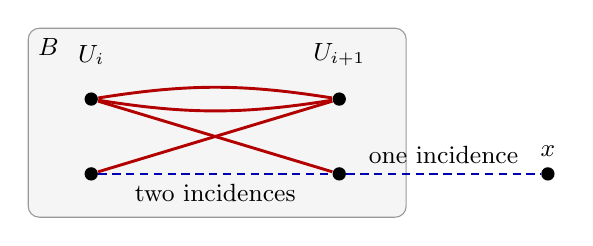
\begin{tikzpicture}[
  marked edge/.append style={draw=red!70!black},
  blue pair/.style={draw=blue!70!black,densely dashed,line width=0.95pt},
  font=\small
]
  \filldraw[fill=black!4,draw=black!40,rounded corners=4pt]
    (-0.65,-0.55) rectangle (4.15,1.85);
  \node[anchor=north west] at (-0.65,1.85) {$B$};
  \node at (0.15,1.51) {$U_i$};
  \node at (3.3,1.51) {$U_{i+1}$};
  \node[graph vertex] (a) at (0.15,0.95) {};
  \node[graph vertex] (b) at (0.15,0) {};
  \node[graph vertex] (c) at (3.3,0.95) {};
  \node[graph vertex] (d) at (3.3,0) {};
  \node[graph vertex,label=above:$x$] (x) at (5.95,0) {};
  \draw[marked edge] (a) to[bend left=9] (c);
  \draw[marked edge] (a) to[bend right=9] (c);
  \draw[marked edge] (a)--(d);
  \draw[marked edge] (b)--(c);
  \draw[blue pair] (b)--node[below] {two incidences} (d);
  \draw[blue pair] (d)--node[above] {one incidence} (x);
\end{tikzpicture}
\caption{A blue edge between consecutive parts contributes twice to
the degree sum on $B$. A blue edge from $x\notin B$ to $B$ contributes
once. Both copies of a marked pair contribute to marked degree.}
\label{fig:multigraph-cut}
\end{figure}


We first bound the total outside contribution after charging $b_x$ against
the core capacity. Suppose $k_x=1$ and $x$ has a marked edge to a vertex of $B$.
We show that $b_x\ge a_*+1$. Let $j$ be the sole index in the signature of $x$, and write $xy$ for
its marked edge with $y\in U_i$. Since $\{j,i-1,i+1\}$ covers the
cycle, $i=j\pm2$. Of the two cycle neighbors of $c_j$, let $c_k$
be the one nonadjacent to $y$. For each $u\in U_j$ the edge $c_ku$
is marked. Comparing it with $xy$ gives $xu$ or $yu$ in the support.
The edge $xy$ uses one of the $s_i$ extra incidences at $y$, so
$y$ has at most $s_i-1$ neighbors in $U_j$. At least
$a_j-s_i+1\ge a_*+1$ vertices of $U_j$ are therefore adjacent to
$x$. Each of these edges is blue, since $\{j,j-1,j+1\}$ does not
cover the cycle. If $xy$ is marked with $k_x=1$ and $k_y=2$, the union of their
signatures is a vertex cover of the cycle and hence has size three.
Whenever the union on an outside marked edge has size three, its two
omitted positions are nonconsecutive. Every red edge from either
omitted anchor into $B$ forces its other end to be adjacent to at least
one end of the outside marked edge. The core neighborhoods of those
ends therefore cover three classes. The other two classes have total
size at most $D$, so the three classes contain at least $|B|-D=D+a_*$
vertices. Each end uses one degree unit on the outside marked edge,
and so each sees at least $a_*+1$ vertices of $B$. If the end of
signature size one has no marked edge into $B$, these pairs are blue.

We redistribute the quantities $h_x-b_x$ over vertices outside $B$.
A vertex of signature size one with a marked core neighbor or a
marked neighbor of signature size two has $b_x\ge a_*+1$. Since
$h_x+b_x\le D$, it retains a contribution at most $R-2$. Any other
vertex of signature size one sends $\frac{1}{2}$ per marked copy to
its neighbors, all of which have signature size at least three. Its
remaining contribution is at most $\frac{D}{2}$. A vertex $x$ of
signature size zero with a marked neighbor of signature size three
has $b_x=Q_x\ge a_*$ by the comparison with the two omitted anchors.
It distributes its positive contribution uniformly over its marked
edges. Since $h_x\le D-Q_x$, the amount per copy is at most
$\frac{2R}{D+R}$. The other vertices of signature size zero use the
same rule, with at most one per copy and with recipients of
signature size at least four. We discard any negative contribution
left at a vertex of signature size zero.

A recipient of signature size three with a marked neighbor of
signature size zero also sees at least $a_*$ vertices of $B$, so it
has at most $\frac{D+R}{2}$ marked copies outside $B$. Multiplying
this bound by the larger of the two sending rates shows that it
receives at most $\max\{\frac{D+R}{4},R\}$. If it has no marked
neighbor of signature size zero, it receives at most $\frac{D}{2}$.
A recipient with at least four positions receives at most $D$.
Adding each recipient's own contribution, at most $D$, shows that
the total contribution at every outside vertex is at most
$k_x\max\{\frac{D}{2},R\}$ for $R\le D$. By \eqref{eq:multi-core-cut},
\begin{equation}\label{eq:multi-rough-discharge}
2m\le D|B|-2L+\max\left\{\frac{D}{2},R\right\}K.
\end{equation}

In the graph on $B$ consisting of the marked pairs, the minimum size
of a vertex cover is at least $D+q$, where $q=a_*-\frac{L}{a_*}$
when $a_*>0$. In fact, any independent set in this graph with $x_i$
vertices in $U_i$ satisfies $\sum_i x_i x_{i+1}\le L$, and
\[
 \sum_i x_i x_{i+1}\ge a_*\left(\sum_i x_i-D\right).
\]
The difference between the two sides is affine in each $x_i$ on
$[0,a_i]$, so it suffices to check the inequality for each $x_i$ in
$\{0,a_i\}$. At such a point, delete one occupied class from each
consecutive occupied pair until the occupied classes are pairwise
nonconsecutive. An edge with both classes occupied accounts for a
product $a_i a_{i+1}$, and either deletion removes at most
$\frac{a_i a_{i+1}}{a_*}$ vertices. The remaining classes contain at
most $D$ vertices because any two nonconsecutive classes have a
common neighboring class. Hence any independent set has size at most
$D+\frac{L}{a_*}$. Subtracting from $|B|=2D+a_*$ gives the bound on
the vertex cover number. The argument applies also with enlarged
classes below. The core neighborhoods of the two ends of an outside
marked edge cover all marked pairs in $B$, so $Q_x+Q_y\ge D+q$ for
every such edge $xy$.

For a sharper estimate, let $q\ge0$ be any lower bound on the vertex
cover number minus $D$. Vertices of signature size zero, and vertices
of signature size one with no marked neighbor in $B$ or of signature
size two, now send only their positive contributions. They distribute
these contributions uniformly over their marked copies, all of which
meet vertices of signature size at least three. At a sender $x$ with
positive contribution, $b_x=Q_x$, so $Q_x<h_x\le D-Q_x$.
Each of its marked neighbors has at least $D+q-Q_x$ core neighbors
and hence at most $Q_x-q$ outside marked copies. In particular,
$q\le Q_x<\frac{D}{2}$. If $q\ge\frac{D}{2}$, there is no positive
transfer. Set $u=(\frac{D}{2}-q)_+$. A recipient receives at most
\[
 C(u)=\frac{2u^2}{\frac{D}{2}+u}.
\]
Indeed, the amount sent per copy is
$1-\frac{Q_x}{h_x}\le\frac{D-2Q_x}{D-Q_x}\le\frac{D-2q}{D-q}$,
and the recipient has at most $u$ outside marked copies. If $a_*>0$
and $q\ge a_*-\frac{L}{a_*}$, then $u\le\frac{R}{2}+\frac{L}{a_*}$.
Since $0\le C'(u)\le2$ for $u\ge0$, it follows that
$C(u)\le\frac{R^2}{D+R}+\frac{2L}{a_*}$.
More generally, if there are $c$ possible recipients, positive
transfer requires $Q_x<h_x\le c(Q_x-q)$. This is impossible for $c=1$,
and for $c=2$ it implies $Q_x>2q$. For two recipients the amount
sent per copy is at most $\frac{D-4q}{D-2q}$ whenever transfer
is possible. Multiplying by $u$ shows that each recipient receives
at most $\max\{0,\frac{D-4q}{2}\}$.

For each $x$ outside $B$, discard any negative contribution left
at a sender and denote by $\ell_x$ the difference between
$\frac{k_xD}{2}$ and the resulting contribution of $x$.
A vertex of signature size one has $\ell_x\ge t+2$ for
$t=\frac{D}{2}-R$ and $R\ge3$. Indeed, it either retains at most
$R-2$ or sends its whole positive contribution and retains zero.
For signature size two, $\ell_x=D-h_x+b_x\ge2b_x\ge2$.
A recipient of signature size $k$ has
$\ell_x\ge(\frac{k}{2}-1)D-C(u)$, or the bound obtained using the
smaller transfer estimate when $c\le2$. Substituting
$\sum_x(h_x-b_x)\le\frac{DK}{2}-\sum_x\ell_x$ into
\eqref{eq:multi-core-cut} and using $|B|=\frac{5D-R}{2}$ gives
\begin{equation}\label{eq:multi-loss-budget}
 2L+\frac{D}{2}(R-K)+\sum_x\ell_x\le2\mu.
\end{equation}

\subsubsection{A joint bound on the core and its exterior}
\label{app:multi-joint}

Write $r=\frac{R}{D}$, $j=\frac{\sum_i j_{c_i}}{D}$,
$g=\frac{m}{D^2}-\frac{5}{4}$, and $\lambda=\frac{L}{D^2}$.
The outside anchor pairs and the extra marked copies at the anchors
use disjoint units of the capacity $R$, so $\frac{K}{D}\le r-j$.
If $\frac{1}{2}\le r\le1$, then
\begin{equation}\label{eq:multi-joint}
 2g+2\lambda\le
 \frac{1+r}{2+r}\,r\left(r-\frac{1}{2}\right)
 -\frac{1+r^2}{2+r}\,j .
\end{equation}

To prove this, divide all vertex counts and degrees by $D$, and all
edge counts by $D^2$. Write $\eta=\frac{1-r}{2}$, $v=\frac{1+r}{2}$
and $\rho=\frac{2r}{1+r}$. An outside marked edge whose signatures
have union of size three has two ends each with normalized core
degree at least $\eta$. Each end has outside marked degree at most
$v$.

Let $x$ count the vertices of signature size one with a marked
neighbor in the core or a marked neighbor of signature size two.
Their total contribution in \eqref{eq:multi-core-cut}, in the
normalized units, is denoted by $C_1$. Each of these vertices has
at least $\eta$ blue pairs into the core, and $C_1\le rx$. Let
$p_2,p_3$ count the marked edges from these vertices to vertices of
signature size two and of signature size at least three, respectively.
Let $n_2$ count their neighbors of signature size two via a marked
edge. Also let $z_3,z_0$ count the vertices of signature size three
and of signature size zero, respectively, that meet a marked edge
joining these two groups. Denote the count of such edges by $p_{03}$.
The three groups counted by $n_2,z_3,z_0$ are disjoint. Each of their
vertices uses at least $\eta$ of the core capacity by the comparison
with the two omitted anchors, and $p_2\le v n_2$ and
$p_{03}\le v\min\{z_0,z_3\}$.

By \eqref{eq:multi-core-identities}, the total normalized capacity
of the core after reserving its consecutive pairs is at most
$\frac{r}{2}$. Deduct the core capacity used by the groups counted
by $x,n_2,z_3,z_0$. To bound $C_1$, add the exterior marked
counts $p_2+p_3$ and deduct the blue core pairs at the vertices
counted by $x$. This gives
$C_1\le\frac{r}{2}-2\eta x-\eta(n_2+z_3+z_0)+p_2+p_3$.
With $\theta=\frac{2r-1}{2+r}$ and $c=r-\theta=\frac{1+r^2}{2+r}$,
take weights $1-\theta,\theta$ on the two bounds for $C_1$ to get
\begin{equation}\label{eq:multi-joint-first}
 C_1\le cx+\frac{\theta r}{2}
     +\theta(p_2+p_3)-\theta\eta(n_2+z_3+z_0).
\end{equation}

For the other outside vertices, use the redistribution leading to
\eqref{eq:multi-rough-discharge}. A vertex of signature size two
retains at most one. Assign $\theta p_2-\theta\eta n_2$ in
\eqref{eq:multi-joint-first} to the group of such vertices. Since
$p_2\le v n_2$, its additional contribution is at most $\theta r$
per vertex, or at most $c=\frac{1}{2}+\frac{\theta r}{2}$ per signature
position after adding the original contribution.

For a vertex of signature size at least four, let $d_1$ be its
marked degree to the group counted by $x$. None of those edges
transfers any contribution to it, so its own and received
contributions sum to at most $2-d_1$. The corresponding bound for a
vertex of signature size three with no marked neighbor of signature
size zero is $\frac{3}{2}-\frac{d_1}{2}$. Adding the corresponding
$\theta d_1$ from $\theta p_3$ gives at most $c$ per signature
position in both cases, since $c\ge\frac{1}{2}$ and $\theta\le\frac{1}{3}$.

For the group counted by $z_3$, write $d_{1,3}$ for its marked
degree to the group counted by $x$. The vertices counted by $z_3$
have outside marked degree at most $v$ and receive at most
$\frac{1}{2}$ per marked copy, except for edges to the vertices
counted by $z_0$, which can transfer up to $\rho$ each. The total
after adding the corresponding terms of \eqref{eq:multi-joint-first}
is at most
\[
 \left(1+\frac{v}{2}\right)z_3
 -\left(\frac{1}{2}-\theta\right)d_{1,3}
 +\left(\rho-\frac{1}{2}\right)p_{03}-\theta\eta(z_3+z_0).
\]
Use $z_0\ge\frac{p_{03}}{v}$, then $p_{03}\le v z_3$, to
bound this by $(1+\rho v-2\theta\eta)z_3=3c z_3$. The second
substitution is valid because
$\rho-\frac{1}{2}-\frac{\theta\eta}{v}\ge0$ for $\frac{1}{2}\le r\le1$.
This accounts for all terms of \eqref{eq:multi-joint-first}.
The vertices of signature size one outside the group counted by
$x$ retain at most $\frac{1}{2}$ each. Thus the right side of
\eqref{eq:multi-core-cut}, divided by $D^2$, is at most
$\frac{5-r}{2}-2\lambda+c(r-j)+\frac{\theta r}{2}$.
Subtracting $\frac{5}{2}$ proves \eqref{eq:multi-joint}.

\subsubsection{Enlarging the Five Parts}

Every vertex $x$ whose signature consists of two nonconsecutive indices $i,j$,
with $b_x<a_*$, and with complete host adjacency to both $U_i$ and
$U_j$, is put into their common neighboring class. We show that
every pair joining consecutive enlarged classes is still an edge
of the simple support. For two newly
added vertices $x,y$ in consecutive classes $p,p+1$, choose a marked
neighbor of $x$ in $U_{p-1}$ avoiding the at most $s_{p+1}$ neighbors
of $y$ there. Then choose a marked neighbor of $y$ in $U_{p+2}$ avoiding
the neighbors of the first choice and of $x$. The latter two vertices
have at most $s_{p-1}+s_p$ neighbors in that class. Both choices
are possible by \eqref{eq:multi-core-identities} and $b_x,b_y<a_*$.
The two chosen marked edges force $xy$. The old--new pairs are
complete by the inclusion rule. A prime denotes enlarged quantities.
In particular each inclusion reduces $R$ and $K$ by two. The old
marked anchor stars can still be used.

Here are the comparisons for a remaining vertex of signature size two. If its
positions $\{i,j\}$ are nonconsecutive, $b_x<a_*$, and
it remains outside, it omits at least one point of both $U_i$ and $U_j$.
Indeed an omitted point in $U_i$, through its marked spoke, bounds the
number of distinct marked neighbors of $x$ in $U_j$ by $s_i$. This
contradicts complete adjacency to $U_j$ since $a_j-b_x>s_i$.
The same comparison with an omitted point works for neighbors in
$U'_j$, using the new bound $s_i'$. Its marked core neighbors can only
lie in $U_i'\cup U_j'$. To see this, take positions $\{4,1\}$, so that
comparison with the cycle excludes $U_0'$. A mark to $U_2'$ would force
at least $a_4-s_2'$ host neighbors of $x$ in $U_4$ by the star from
$c_0$. At most $s_1'$ of these are marked, contrary to $b_x<a_*$
by \eqref{eq:multi-core-identities}. A mark to $U_3'$ is excluded by
reflection. Both anchor pairs of $x$ are blue. If one were marked,
the marked star into the other designated class, based at an anchor
missing the first, would force complete adjacency to that other
class. Each of the two marked-neighbor counts into the designated
classes is at most the slack of the opposite class. Thus
\begin{equation}\label{eq:multi-low-blue-outside}
 Q_x\le s_i'+s_j'+b_x.
\end{equation}
If $xy$ is marked with $y\in U_i'$, every omitted old $U_j$ vertex must
see $y$, again by its marked spoke. At most $s_i'-1$ such vertices
can be omitted since $xy$ already consumes one unit at $y$. It follows
that $b_x\ge a_j-2s_i'+1\ge a_*-s_i'+1$. The same omitted vertices
also give
\begin{equation}\label{eq:multi-rectangle}
 I+b_{x,j}\ge a_j-s_i'\ge a_*,
\end{equation}
where $I$ counts host edges inside the enlarged core other than its
reserved base edges and
$b_{x,j}$ counts the blue neighbors of $x$ in old $U_j$.

A vertex with $b_x<a_*$ and signature $\{0,1\}$ can have marked edges
into the enlarged core only to $U_3'$. The cycle excludes marked edges to $U_0'$ and
$U_1'$. A mark to $U_2'$ forces at least $a_0-s_2'$ blue neighbors
in $U_0$ by the star from $c_4$, and a mark to $U_4'$ is excluded
by the reflected comparison. If there is a marked neighbor in $U_3'$,
the two ends of that mark must cover the marked $U_0$--$U_1$ pairs.
If the union of their neighborhoods omits $t_0$ vertices of $U_0$
and $t_1$ vertices of $U_1$, then all $t_0t_1$ pairs between these
omitted sets are blue. Thus $t_0t_1\le L$ and one of $t_0,t_1$ is at
most $\sqrt L$.
The neighbor in $U_3'$ can pay for at most $s_3'-1$ wrong-class
adjacencies in either part after accounting for the selected mark.
Thus $b_x\ge a_*+1-\sqrt L$. Finally, if a remaining outside vertex
has no enlarged core mark, a marked outside neighbor has $Q\le D-1$.
The old vertex-cover bound therefore gives $b_x=Q_x\ge q+1$.

Reserve one base copy for each pair in consecutive enlarged
classes, choosing a marked copy whenever possible. Let $L'$
count the unmarked base copies. Let $I$ count the other host
edges inside the enlarged core, $P$ count the marked ones among
them, $L_{\rm cut}$ count the unmarked copies across the cut of
the enlarged core, and $f$ count the marked copies with both ends
outside. There are $\frac{D|B'|-A'}{2}-L'$ marked base copies.
The number of marked copies across the cut is at most
$A'-2I-L_{\rm cut}$, since the edges counted by $I$ each use two
units of the remaining core capacity $A'$. Adding $P$ and $f$ and
using \eqref{eq:multi-core-identities} gives
\begin{equation}\label{eq:multi-extra-capacity}
 \mu\ge \frac{R'D-2A'}{4}+L'+(2I-P)+L_{\rm cut}-f
 \ge L'+I+L_{\rm cut}-f .
\end{equation}
When $R'=1$, all but one class have zero extra capacity. If all
outside signatures are singletons, outside marks are impossible.
Any non-base mark in the only positive-capacity class or from
outside to that class misses the opposite cycle edge, so only marked
base copies remain. Their total is at most $f(D)$.

\subsubsection{The half-degree threshold}
\label{app:multi-half}

We prove that for odd $D\ge9$, a counterexample has $R>\frac{D+1}{2}$ on
every anchored cycle. If $R=1$, outside signatures have size at most
one and no outside vertex can have signature zero in the marked
endpoint host. The $R'=1$ base count above applies without enlargement.
Assume $R\ge3$ and $t\ge-\frac{1}{2}$. If $t\ge\frac{1}{2}$,
\eqref{eq:multi-rough-discharge} gives $L\le \frac{D}{2}-\frac{5}{4}$ and $R-K\le1$.
Also $a_*\ge3$ and $\frac{L}{a_*}<2$. For $t=-\frac{1}{2}$ and $D\ge13$, it gives
$L\le\frac{5D-9}{8}$ and $\frac{L}{a_*}<\frac{5}{2}$, with $a_*\ge3$. In both cases
$q>0$. The remaining case $(D,R)=(9,5)$ has $a_*=2$, $L\le4$ and
$q\ge0$. Also $K\le5$, so at most one recipient is possible there.
In all cases $C(u)\le \frac{D}{2}$ and the losses in
\eqref{eq:multi-loss-budget} are nonnegative. That inequality gives
$R-K\in\{0,1\}$ and $L\le \frac{D}{2}-\frac{5}{4}$.

There is at most one vertex of signature size at least three.
Indeed, $\frac{R^2}{D+R}\le \frac{D}{6}$ for $t\ge\frac{1}{2}$ and is at most $\frac{D}{6}+\frac{1}{2}$
for $t=-\frac{1}{2}$. The loss of three recipients, with $2L$ included,
would be at least $D-\frac{3}{2}$, since $a_*\ge3$. With two recipients,
the improved bound gives total loss with $2L$ at least $D-1$.
Both bounds exceed the budget. With one recipient no positive
transfer occurs, and its size is exactly three.

Suppose first there is one vertex of signature size three, say $z$. Let $a$
count vertices of signature size one. Parity and the budget force $a$ even
and $R-K=0$. The lower bound on the total loss is
$\frac{D}{2}+R-3+a(t+1)$. For $a\ge2$ this exceeds $D-\frac{5}{2}$, so $a=0$.
We show that every vertex with $k_x=2$ is included in the enlarged core.
For $t=-\frac{1}{2}$ the budget forces $L=0$ and each vertex of signature size two
to have one blue neighbor. A remaining vertex with nonconsecutive
signature positions and $b_x<a_*$ would have two blue anchor pairs.
The other remaining types
violate $b_x\ge a_*+1-\sqrt L$ or $b_x\ge q+1$. For $t\ge\frac{1}{2}$ a
remaining vertex with nonconsecutive signature positions, $b_x<a_*$
and a marked edge to the core satisfies
$b_x\ge a_*+1-s_i'\ge t+\frac{3}{2}$. Indeed, $R'=K'$ and the slack
at each position counts the remaining vertices that use it.
There are $\frac{R'-3}{2}$ such vertices of signature size two,
and at most one more can use that position, namely $z$.
Together with the loss of $z$ and the other vertices of signature size two
this gives a loss of at least $D+t-2>D-\frac{5}{2}$. A remaining vertex with $b_x\ge a_*$
costs at least $2a_*$ and a remaining vertex of either other type
costs at least $2a_*+2$ with $2L$ included. These also exceed the
budget after adding the other vertex losses.

The resulting enlarged core has $R'=3$, with three units at the
positions of $z$. Write $D=2d+1$. If the omitted positions are
nonconsecutive, the three classes of positive capacity have sizes
$d+1,d,d$, base count $f(D)-D$ and extra capacity $3d+1$.
If $zy$ is marked outside, then the vertex of signature size zero $y$ has
only blue core pairs. The two omitted anchor stars force
$Q_z'+Q_y'\ge3d+1-L'$, since each omitted point of those three
classes consumes a distinct blue base pair. Also $f\le D-Q_z'$.
Thus $L'+L_{\rm cut}-f\ge d$. If there is no outside mark, only
$z$ remains outside. The extra marks either all touch $z$ and
number at most $D$, or there is a marked non-base copy inside
the core. No same-class mark is possible by the opposite cycle
edge. A mark from the class of size $d+1$ to one of size $d$
blocks any mark from $z$ to those two classes. Its endpoints use
their only extra units and every possible edge joining their marked edge to
such a mark from $z$ would use one of those units. The total number
of extra marks is then at most $\frac{3d+1+d}{2}\le D$. If there are
only repeated internal marks between the two consecutive size-$d$
classes, one of those repetitions blocks marks from $z$ to the
size-$(d+1)$ class by the same comparison. The extra marks then
use at most $2d$ units and still number at most $D$.

If the two omitted positions are consecutive, put the three
positive positions at $0,1,2$. The base count is $f(D)-(D-1)$.
No outside mark sees the omitted cycle edge. A mark from $z$ to
$U_1'$ would also miss that edge, so $h_z\le D-1$ and $z$ marks
to $U_0'$ or $U_2'$. A mark to $U_0'$ forces $z$ to see every
vertex of $U_2'$ having a marked neighbor in $U_3'$ by comparison
with the marked edges to $U_3'$, where $s'_3=0$. If such a
neighbor is absent at some vertex of $U_2'$ then $L'\ge d+1$
and \eqref{eq:multi-extra-capacity} suffices. Otherwise the
adjacency to $U_2'$ is complete. If these pairs are all blue the
cut costs at least $d$. If one is marked, reflection forces
complete adjacency to $U_0'$ too. The two classes now have no
remaining extra capacity and the middle class cannot have a
same-class mark. The only extra marks meet $z$ and number at most
$D-1$. In every subcase $\mu\ge d$ suffices, since its fractional
part is $\frac{1}{4}$.

Suppose now that there is no vertex with three or more positions.
Then there are no vertices of signature size zero. If all outside vertices have
two positions, the budget and parity give $R-K=1$ and there are
$n=\frac{R-1}{2}$ outside vertices. The total number of unmarked host
edges is at most $\frac{D-5}{4}$. Indeed, summing the differences
between $D$ and the marked degree over the $\frac{5D-1}{2}$ vertices
counts at least twice the number of unmarked host edges.
Hence $\sum b_x\le \frac{D-5}{4}-L<a_*-\sqrt L$,
using $a_*\ge\frac{D-1}{4}$. Every outside vertex has a marked core
neighbor by the vertex-cover bound, while the comparison for
consecutive positions excludes those positions. Apply the enlargement
rule to every eligible vertex. Two remaining vertices cannot be joined
by a marked edge.
Their combined old-core neighborhood would have to omit at most
$\sqrt L$ points in at least three classes, since two consecutive
omitted sets have product at most $L$. In any class outside the
intersection of their two designated class sets, their combined
neighborhood omits at least $a_*-b_x-b_y>\sqrt L$ points. The
intersection has at most two classes. If no vertex remains, $R'=1$.
Otherwise take a marked edge to $U_i'$ from a remaining vertex $x$
of positions $\{i,j\}$. Each original vertex of signature size two pays
one blue anchor pair to $L'+L_{\rm cut}$. For $x$ choose its pair
to $c_i$, which is disjoint from its $b_{x,j}$ pairs. By
\eqref{eq:multi-rectangle} and \eqref{eq:multi-extra-capacity},
$\mu\ge n+a_*=\frac{D-1}{2}$, as required.

It remains to consider $a>0$ vertices of signature size one and no
vertex of signature size three. If $a$ is even then $R-K=1$ and the loss
is at least $\frac{D}{2}+R-1+a(t+1)>D-\frac{5}{2}$. Hence $a$ is odd and $R=K$.
Apply the enlargement rule and let $n$ be the number of remaining
vertices of signature size two, so $R'=a+2n$. After subtracting the base
losses, \eqref{eq:multi-loss-budget} implies
\[
 2L+\sum_{\rm remaining\ two}(\ell_x-2)
 \le T=2a_*-\frac{5}{2}-a(t+1).
\]
A vertex with $b_x\ge a_*$ contributes at least $2a_*-2>T$ to the
left side. For a vertex with $b_x<a_*$ and consecutive signature
positions, or a vertex without a marked edge to the core, its
contribution together with $2L$ is at least $2a_*$ by the bounds
$a_*+1-\sqrt L$ and $q+1$, respectively. Therefore each remaining
vertex with $k_x=2$ has $b_x<a_*$, nonconsecutive signature positions,
and a marked edge to the core. Its two anchor pairs are blue.

If two such vertices $x,y$ mark to one another, their signatures
are distinct. Equation \eqref{eq:multi-low-blue-outside} shows that
their marked-neighbor counts in the old core sum to at most
$2R'-n$, since any shared position has $s_i'\le a+n$.
Consequently
\[
 b_x+b_y\ge D+q-2R'+n\ge a_*+2t+n-\frac{L}{a_*}.
\]
The budget gives $b_x+b_y\le \frac{T}{2}-n+4-L$. These contradict for
$n\ge2$, $a\ge1$ and $t\ge-\frac{1}{2}$.

Suppose $xy$ is marked, where $k_x=1$ and $y$ is a remaining
vertex with $k_y=2$. After a rotation of the cycle, the signature
of $x$ is $\{0\}$ and that of $y$ is $\{1,3\}$ or $\{2,4\}$. The omitted anchor stars require
complete combined adjacency to the three indicated old classes.
If $x$ has a marked edge to $B$, it has at least $a_*+1$ blue pairs
in $U_0$. The designated class $U_1$ or $U_4$ for $y$ is short of
at least $a_*-b_y$ of its vertices. These must be covered by
additional blue pairs of $x$, since $x$ only marks to $U_2$ or
$U_3$ in the old core. If $x$ has no marked edge to $B$, the
three required classes have at least $D+a_*$ vertices and $y$
has at most $R'$ marked neighbors there. Both cases imply
$b_x+b_y\ge2a_*+1$. The budget then requires at least
$D+a(t+1)-2>D-\frac{5}{2}$ in losses after including the other vertices.
There are also no marks between two vertices of signature size one.
Thus $f=0$. If $n>0$, then \eqref{eq:multi-rectangle} and the blue edges
from one vertex of signature size one to $B$ give $I+L_{\rm cut}\ge2a_*+1>\frac{D}{2}$.
If $n=0$ and $a\ge3$ then $L_{\rm cut}\ge3(a_*+1)>\frac{D}{2}$.
The last possibility is $R'=a=1$, already settled.


\subsubsection{Small-degree slack thresholds and a single repeated pair}
\label{app:multi-small-slack}

For $(D,R)=(11,7),(15,9)$, write $D=4k+3$ and $R=2k+3$.
Here $k=2,3$ and $a_*=k$. Equation \eqref{eq:multi-rough-discharge}
gives $L\le9,13$, respectively. For $L<D$, the old marked
vertex-cover number satisfies the improved bound
\begin{equation}\label{eq:multi-small-cover}
 \tau\ge D+a_*-\max\{0,\lfloor\sqrt L\rfloor-1\}.
\end{equation}
To prove it, consider an independent set of size $\alpha>D$ in
the marked old core, with $x_i$ points in $U_i$. It occupies a
consecutive pair of positions, since any two nonconsecutive classes
have total size at most $D$. If the occupied positions induce a
connected graph, summing $x_i x_j\ge x_i+x_j-1$ on a spanning tree
gives $L\ge\alpha-1\ge D$. If they induce a disconnected graph,
the occupied positions consist of one edge and one isolated point.
The two classes of the edge cannot contribute their own anchors,
because the anchor spokes to the adjacent class are marked. Either
of these classes and the isolated class now contribute at most
$D-1$ points. Hence the adjacent classes
each contribute at least $\alpha-D+1$ and $L\ge(\alpha-D+1)^2$.
Subtracting the upper bound for $\alpha$ from $|B|$ proves
\eqref{eq:multi-small-cover}.

Use $q=\tau_{\rm lo}-D$ with $\tau_{\rm lo}$ the right-hand side
of \eqref{eq:multi-small-cover} in the sharper discharging.
Initially $q\ge0$. A vertex with $k_x=1$ has loss at least
$\frac{1}{2}$, and one with $k_x=2$ has loss at least $2$. All other
losses are nonnegative. Thus $L\le 2k$ and $R-K\in\{0,1\}$. For $c\ge2$
potential recipients, positive transfer requires
$h_x\le c(Q_x-q)$ and $Q_x>\frac{cq}{c-1}$. Substituting the integer
values $Q_x<\frac{D}{2}$ bounds the number of recipients as follows.

For $D=11$, two recipients with $L\le3$ have $q=2$. The only
possible $Q_x$ for a positive transfer is $5$, so the rate
is at most $\frac{1}{6}$ and each recipient can receive on at most
three edges. Their combined loss is at least $10>\frac{17}{2}$.
At $L=4$ even one recipient's loss with $2L$ is at least
$\frac{11}{2}-\frac{81}{20}+8>\frac{17}{2}$. For $D=15$, three recipients with
$L\le3$ have $q=3$ and each can receive at most $\frac{18}{7}$.
Their combined loss is greater than $\frac{25}{2}$. When $L\ge4$,
$q=2$ and the recipient bound is $\frac{33}{8}$ each, again exceeding
$\frac{25}{2}$ with the $2L$ term. With two recipients and $q=3$,
only $Q_x=7$ can give a positive transfer, at a rate of at most
$\frac{1}{8}$ for at most four edges per recipient. With two recipients
and $q=2$, each can receive at most $\frac{7}{2}$, and $L\ge4$.
Both violate the budget, so there is at most one vertex of signature size
three in either degree, with no positive transfer.

We give the remaining cases for $D=11,15$ in terms of
$d=\frac{D-1}{2}=2k+1$. A contradiction follows from $\mu\ge d$.
We use two consequences of enlargement. First, each absorbed vertex
$x$ contributes at most $D-h_x$ new blue consecutive pairs and at
least one such pair, since one of its two anchor pairs is blue.
Thus, if $p$ vertices are absorbed,
\begin{equation}\label{eq:multi-new-blue}
 L+p\le L'\le L+\sum_{x\ {\rm absorbed}}(D-h_x).
\end{equation}
The vertex cover number of the enlarged marked core is at least
$\tau'=D+a_*'-\frac{L'}{a_*'}$, rounded up to the next integer,
where $a_*'=\frac{D-R'}{2}$. Second, if all $f$ outside marked
edges meet one vertex and that vertex has at most $p$
distinct outside marked neighbors, then
\begin{equation}\label{eq:multi-center-cut}
 f\le\frac{p}{p+1}(2D-\tau').
\end{equation}
Indeed, one of its neighbors has outside marked degree at least
$\frac{f}{p}$, and the outside marked degrees of the two ends sum to
at most $2D-\tau'$. The bound is immediate when $p=0$.

Suppose there is one vertex $z$ of signature size three. Write $a$
for the number of vertices of signature size one. If $R-K=1$, the
unused anchor capacity and the loss at $z$ already sum to $D$, so
$R=K$ and $a$ is even. The $k-\frac{a}{2}$ vertices of signature size
two, the $a$ vertices of signature size one, and $z$ give total
loss at least $4k+\frac{3}{2}-\frac{a}{2}$. After these losses,
\eqref{eq:multi-loss-budget} allows at most $\frac{a}{2}-1$ more.
It follows that $a=2,4$, or that $a=6$ and $k=3$.

For $a=2,4$ we have $L=0$ and every vertex of signature size two
has $b_x=1$. These vertices have nonconsecutive positions and
enter the enlargement. Indeed, for consecutive positions a marked
edge into the enlarged core requires $b_x\ge k+1$, and an outside
marked edge with no enlarged core mark requires $b_x\ge q+1=k+1$.
A vertex of the nonconsecutive type left outside would have two
blue anchor pairs. When $a=6$ there are no vertices of signature
size two. All outside marks after enlargement meet $z$. Every
vertex of signature size one has at least $k+1$ blue pairs into
$B$, since a vertex without the two listed kinds of marked neighbor
would lose $\frac{D}{2}$, exceeding the available excess loss
$\frac{a}{2}-1$. If a vertex of signature size zero marks to $z$,
its entire core neighborhood is blue and has size at least
$\tau'-D+f$. In these cases $\tau'\ge D$, by
\eqref{eq:multi-new-blue} and the bounds on $L'$ below. The
capacity inequality \eqref{eq:multi-extra-capacity} thus gives
$\mu\ge a(k+1)\ge d$. We may assume that all outside marked
edges join $z$ to vertices of signature size one.

If $a=2$, both vertices of signature size one attain their
minimum loss. Each has marked degree $3k+2$ and exactly $k+1$
unmarked incidences, all blue pairs into $B$. The absorbed
vertices have $D-h_x=1$, so $R'=5$, $a_*'=2k-1$, and
$L'\le k-1$. Each vertex of signature size one has an old core
mark. Otherwise its old core degree would be $k+1$, and every
outside marked neighbor would have at least $D-1$ old core
neighbors by the vertex cover bound with $q=k$. Each could give
only one outside marked copy, and there are at most $k$
possible marked neighbors of this kind.

For a vertex of signature $\{j\}$ and a marked neighbor in
$U_i'$, where $i=j\pm2$, use the comparison with the anchor
star from the opposite side of $c_j$. At least
$a_j'-s_i'+1-L_{\star}\ge2k-L_{\star}$ vertices of $U_j'$
are blue neighbors of the vertex of signature size one. Here
$L_{\star}$ counts the blue pairs of that star into $U_j'$.
As it has only $k+1$ blue neighbors, $L_{\star}\ge k-1$.
Stars for different choices of $j$ or different choices of
$i$ share at most a red edge on the anchor cycle, so their
blue pairs are disjoint. It follows from $L'\le k-1$ that the
two vertices have the same signature and mark to the same
class only. The index of this class is used at most once by
the remaining signatures, namely by $z$. Since $R'=K'$,
$s_i'\le1$. Their total marked degree is consequently at most
$a_i'+f$. By the rounded cover bound,
$\tau'\ge D+2k-1$, so \eqref{eq:multi-center-cut} gives
$f\le\frac{2(2k+4)}{3}$. As $a_i'\le2k+4$, this sum is
strictly less than $6k+4$, a contradiction.

If $a=4$, then $R'=7$, and \eqref{eq:multi-new-blue} gives
$L'\le k-1$. Hence $\tau'\ge D+2k-2$ and
$f\le\frac{4(2k+5)}{5}$, which gives $f\le7$ for $k=2$ and
$f\le8$ for $k=3$. In both cases $L_{\rm cut}\ge4(k+1)$
and \eqref{eq:multi-extra-capacity} gives $\mu\ge d$.
If $a=6$, then $k=3$, $L_{\rm cut}\ge24$ and $f\le15$,
which again suffice.

Suppose there is no vertex of signature size at least three.
There are no vertices of signature size zero, and every vertex
of signature size one has at least $k+1$ blue pairs into the
old core. If $a$ is even, then $R-K=1$, and the base losses
require $a\ge6$, leaving at most $\frac{a}{2}-3\le1$ more.
Enlarge the core by all vertices with nonconsecutive signatures
and $b_x<k$ that are complete to both designated classes.
Each remaining vertex of signature size two with $b_x\ge k$
or with two blue anchor pairs costs at least two beyond the
base loss of two. A remaining vertex with consecutive positions
and a core mark, or without any core mark, costs at least $2k$
beyond its base loss when $2L$ is included, by the bounds
$k+1-\sqrt L$ and $q+1$ for $b_x$. Thus all vertices of
signature size two are absorbed. There are no outside marks and
$L_{\rm cut}\ge a(k+1)$.

If $a$ is odd, then $R=K$. Let $n$ count the remaining vertices
of signature size two after enlargement, so $R'=a+2n$. After
subtracting the base losses, the remaining budget is
\begin{equation}\label{eq:multi-small-odd-budget}
 2L+\sum_{\substack{x\ \text{remaining}\\ k_x=2}}(\ell_x-2)
 \le T=2k-\frac{5}{2}+\frac{a}{2} .
\end{equation}
In the following count, a remaining vertex of signature size two
that has nonconsecutive positions, $b_x<k$, and a marked edge
into the enlarged core has two blue anchor pairs. By
\eqref{eq:multi-low-blue-outside}, its old core degree is at
most $R'+b_x$. A marked edge between such a vertex $y$ and a
vertex $x$ of signature size one requires
$b_x+b_y\ge2a_*+1=2k+1$, by the comparison with the two
omitted anchors in \textbf{Appendix~\ref{app:multi-half}}.

If $a\ge5$ and $n\le1$, then all outside marks meet the sole
remaining vertex of signature size two, if it exists. For $n=0$,
$f=0$. For $n=1,k=2$, $L_{\rm cut}\ge5(k+1)+1=16$.
For $n=1,k=3,a=5$ we have $L\le3$, so a remaining vertex
of signature size two has at least two blue cut pairs, whether
its signature is consecutive or nonconsecutive or it has no
core mark. This gives $L_{\rm cut}\ge22$. If $a\ge7$ and
$k=3$, the vertices of signature size one alone give at least
$28$. In each case $f\le D$ and the capacity inequality suffices.

If $a\ge5$ and $n\ge2$, then $k=3$, $a=5$, $n=2$, and
$T=6$. The two remaining vertices of signature size two have
$b_x,b_y\ge2$. If either has $b_x<3$ or $b_y<3$, it has
nonconsecutive positions and a mark into the enlarged core by
the lower bounds on $b_x,b_y$ for the other types. If the two
vertices have a marked edge between them, the sum of their
outside marked degrees is at most $D-q$ by the old core cover
bound, so $f\le D$. Otherwise, if both have blue degree two,
they use at least four units of the budget $T$. At most one
vertex of signature size one can use the remaining two units
to increase its blue degree from four to five. The comparison
$b_x+b_y\ge7$ forces all outside marked copies to meet that
vertex, so $f\le D$. If instead one of the two vertices has
blue degree at least three, the two vertices exhaust $T$.
The vertices of signature size one all have blue degree four,
preventing a marked edge to the remaining vertex of blue
degree two. Again $f\le D$. In each case the blue cut has at
least 24 edges.

If $a=3$, then $T=2k-1$. Each remaining vertex of signature
size two has blue degree at least two, by the same comparisons.
For $n=2$ we must have $k=3$, $L=0$, and both of those vertices
have blue degree two and nonconsecutive positions with a marked
edge to the enlarged core. All three vertices of signature size
one have blue degree four. None can mark to either remaining
vertex of signature size two. If the two vertices of size two
have a marked edge, their signatures are distinct and share at
most one position, of slack at most $a+n$. By
\eqref{eq:multi-low-blue-outside} their combined old core degree
is at most $2R'-n+4=16<D+q$, also impossible. Hence $f=0$.
For $n=1$ we have $R'=5$, and
\eqref{eq:multi-new-blue} and \eqref{eq:multi-small-odd-budget}
give $L'\le(k-1)+T-2-L\le3k-4$. The resulting cover bounds
are $\tau'\ge14$ for $k=2$ and $\tau'\ge19$ for $k=3$.
Equation \eqref{eq:multi-center-cut} gives $f\le6$ and $f\le8$,
respectively. The blue cut has at least 11 or 14 edges,
respectively, and in the latter case $L'\ge2$ by
\eqref{eq:multi-new-blue}. For $n=0$ there are no outside marks,
so the blue pairs from the three vertices of signature size
one suffice.

Finally, let $a=1$, so $T=2k-2$. The lower bounds for vertices
with consecutive positions or with no enlarged core mark
exclude them when their blue degree is less than $k$. If a
remaining vertex $y$ has $b_y\ge k$, its loss above two uses
all of $T$. It is the only remaining vertex of signature size
two, with $b_y=k$ and $h_y=D-k$. We have $L=0$, there are $k$
absorbed vertices, and $L'\le k$. The vertex $x$ of signature size
one has $b_x=k+1$ and $h_x=D-b_x$. Now $R'=3$. If $f=0$, the
blue cut has at least $2k+1=d$ edges. If $f>0$, all outside
marks run between $x$ and $y$. Rotate so that their signature union
is $\{0,2,3\}$. The three corresponding slacks are one and all
other slacks are zero. Put $A_i=U_i'$ for $i=0,2,3$. The sizes
are $d+1,d,d$, respectively. Let $w$ count their vertices
with no red pair to either omitted anchor. These missing red
pairs give distinct blue base pairs, so $w\le L'$. Write
$Q_x',Q_y'$ for the enlarged core degrees. The omitted anchors
force the union of the two neighborhoods to cover at least
$3d+1-w$ vertices of $A_0\cup A_2\cup A_3$. Each end has at most
$D-f$ core neighbors, so $Q_x',Q_y'\ge d+f-w$ and
$2f\le d+1+w$. If one end has no core mark, its blue cut pairs
and $L'\ge w$ give $\mu\ge d$.

Assume both ends have a core mark. If the signature of $x$
is $\{0\}$, then $x$ can only mark into $A_2$ or $A_3$.
Take a marked neighbor in $A_2$, reflecting if necessary.
Its unique extra degree unit is used by this edge, so the
red star from $c_4$ into $A_0$ forces $x$ to see each of its
red neighbors in $A_0$, all through blue pairs. If the star
has $w_0$ blue pairs, this gives at least $d+1-w_0$ blue cut
pairs at $x$. The only available core marks at $y$ go to
$A_0$, by comparison with the cycle edges. At most $w_0$
vertices there still have a degree unit free for $y$. Thus
$L'+L_{\rm cut}-f\ge L'+d+1-w_0+Q_y'-w_0-f\ge2d+1-2w_0\ge d$,
using $w_0\le L'\le k$ and $d=2k+1$.

Otherwise, reflect to give $x$ signature $\{2\}$. It can
mark only into $A_0$. Choose a marked neighbor $u\in A_0$.
The red star from $c_3$ into $A_2$ forces at least $d-w_2$
blue cut pairs from $x$ into $A_2$, where $w_2$ is the
number of blue pairs of that star. If $uc_1$ is red, comparing
that edge with any proposed mark from $y$ into $A_3$ excludes
all such marks. Indeed, neither $y$ nor the vertex in $A_3$
sees $c_1$, and $u$ has used its only extra unit on $xu$.
Therefore all pairs from $x,y$ into $A_3$ are blue. They
cover at least $d-w_3$ vertices there, where $w_3$ counts the
vertices in $A_3$ without a red pair to an omitted anchor.
The corresponding blue base pairs in $A_3$ are disjoint
from the $w_2$ pairs of the star, so $L'\ge w_2+w_3$.
This gives $\mu\ge 2d-f\ge d$, as $2f\le d+1+L'\le2d$.
If every choice of $u$ instead gives a blue pair $uc_1$,
each marked copy from $x$ into $A_0$ gives a distinct
blue base pair. Now $L'\ge h_x-f$, and the old blue pairs
at $x,y$ give $\mu\ge h_x+b_x+b_y-2f=D+k-2f\ge d$.

If all remaining vertices have $b_x<k$, then $n>0$ is possible
only for $k=3$, with $n\le2$ and each blue degree equal to two.
For $n=1$ an outside mark would force $R'=3$ with three
positive slacks all equal to one. The bound
$b_x\ge a_*+1-s_i'$ preceding \eqref{eq:multi-rectangle}
would then give blue degree at least three. For $n=2$, the
two vertices use all of $T$, so $L=0$ and the vertex of
signature size one has blue degree four. Neither vertex can
mark to it, and their combined old core degree is at most
$2R'-n+4=12<D+q$ if they mark to one another. Thus $f=0$.
If $n>0$, apply \eqref{eq:multi-rectangle} to one remaining
vertex and add the $a_*+1$ blue cut pairs of the vertex of
signature size one. These incidences are disjoint and give
$\mu\ge2a_*+1=d$. If $n=0$, then $R'=1$ and only the base
count is needed. This completes the two cases $D=11,15$.

For $(D,R)=(13,9)$, \eqref{eq:multi-joint} gives
\[
 L\le \mu+\frac{1}{2}\,\frac{1+r}{2+r}R(R-\frac{D}{2})<13,\qquad r=\frac{9}{13} .
\]
It follows from \eqref{eq:multi-small-cover} that $q\ge0$.
For a vertex with $k_x=1$, the initial lower bound on its loss is $-\frac{1}{2}$, so
\eqref{eq:multi-loss-budget} gives $R-K\le2$ and $L\le7$ and
hence $q\ge1$. For completeness, we record the transfer bounds
that reduce this case to the terminal counts in the proof supplement.
If there are $c$ recipients, then $c\le3$, and a sender with positive
contribution has $Q<h\le\min\{13-Q,c(Q-q)\}$. It follows that
$Q\le6$ and that a recipient has outside marked degree at most
$6-q$. With $c=3$, there are no vertices of signature size one.
For $q=1$, each marked edge transfers at most $\frac{5}{9}$, so the
three recipients lose at least $3(\frac{13}{2}-\frac{25}{9})>\frac{21}{2}$.
For $q=2$, each marked edge transfers at most $\frac{3}{8}$, so the
loss is at least $15$. For $c=2,q=1$, each marked edge transfers at
most $\frac{3}{8}$. Here $L\ge4$ and there are at most three vertices
of signature size one, giving combined loss and blue deductions
at least $8+13-2\cdot\frac{15}{8}-\frac{3}{2}>\frac{21}{2}$.
These rates follow by checking $Q\in\{1,\ldots,6\}$ in the minimum
above. If $c=2,q=2$, the only possible pairs $(Q,h)$ are
$(5,6)$ and $(6,7)$, and a positive sender meets both recipients.
They have at most eight outside marked incidences in total, so
there is at most one positive sender, transferring one unit.
The loss bound then forces $L=R-K=0$, three vertices of signature
size one with $h_x=10,b_x=3$, and two recipients of signature
size three with $h_x=13,b_x=0$. The sender leaves at most one
outside marked incidence at the recipients for the three vertices
of signature size one and other neighbors. The three vertices
therefore contribute at least 29 marked copies across the old
core cut, and the recipients contribute at least 18. The sender
and the three vertices of signature size one also contribute at
least $5+9$ blue pairs across that cut. The total is at least 61,
whereas \eqref{eq:multi-core-identities} bounds the capacity of
the cut by $18+2\lfloor\frac{81}{4}\rfloor=58$.

There is thus at most one recipient, with no positive transfer.
The exact integer comparisons and remaining cases are proved in
Sections 2--5 of \emph{The exact bound for degree thirteen with
slack nine} in the proof supplement indexed by \path{PROOF_NOTES.md}.
Section 2 supplies
the cover bounds for the enlarged core, and Sections 3--5 split
according to the number of vertices of signature size one and
the signatures remaining after enlargement. Each case gives
$\mu\ge6$ or the base count for $R'=1$. Consequently $R\ge11$
for degree thirteen. For degree nine, the finite reductions
in \textbf{Appendix~\ref{app:multi-nine}} handle $R=7,9$.

We also need to exclude $b=1$ after taking exactly $m=f(D)+1$
marked copies. The projection to distinct host pairs preserves
both the strong-clique obligation and the anchor classes. If
$b=1$, this projection has exactly $f(D)$ marked pairs. In the
simple equality configuration with class sizes
$(d,d,d+1,d+1,d)$, where $d=\frac{D-1}{2}$, every marked pair has
an endpoint of host degree at least $D$ in the projection.
A second marked copy on it contradicts the host capacity.

The simple equality test in the companion files uses a cycle with
largest old core and identifies the five slack entries under
dihedral symmetry. For $D=9,11$, the only possible exception
to the simple equality configuration is $(1,1,2,1,2)$.
For $D=13,15$, the exceptions can only be $(1,1,2,1,2)$,
$(1,1,3,1,3)$ or $(1,2,2,2,2)$. The last two have total
slack nine. Thus the preceding half-degree and special
slack bounds rule out every exceptional case at $D=11,13,15$
in the multigraph counterexample. At $D=9$, the case $b=1$ with a
triangle-free marked graph in the simple support is ruled out by the fixed
$27$-formula replay in \path{d9_anchor_cases.py}.
With a marked triangle the order is $24$ or $25$ by the
degree-nine order reduction. The only exceptional shape is
$(1,1,2,1,2)$, and the replay with \path{d9_pentagon.py},
\path{--bundles 1 --triangles require}, and
\path{--select s11212} checks its fixed unsatisfiability
proof. This is the case \path{d9_b1_triangle/s11212.json}
in the companion archive. The precise reduction and replay
transcripts are indexed under \emph{A single repeated marked pair}.


\subsection{Enumeration and Boolean Formulas for Multigraphs}
\label{app:multi-finite}
\textbf{Section~\ref{sec:exact}} gives the degree and adjacency constraints used below.
For each case, the verification enumerates the possible integer data
or checks a refutation of the Boolean formula describing those
constraints.

\subsubsection{Maximum Degrees Five and Seven}\label{app:multi-low-degree}

For the 21 configurations in \textbf{Figure~\ref{fig:finite-five-spokes}},
\path{d5_parallel_spoke_bound.py} fixes the six spokes and the edges
between their nonroot endpoints. For one vertex outside the root
neighborhoods it enumerates the vectors $z$ of marked multiplicities
and $u$ of required host incidences as in
\textbf{Subsection~\ref{subsec:exact-small-degree}}. Starting with
$V(0)=0$, the recurrence bounds the additional marked edges at each
remaining capacity vector. Adding the fixed marked edges gives the
21 bounds printed in the figure, whose maximum is 27.

At $D=7$, Section~3 of \path{delta7_parallel_reduction.md} gives the
parameters for the recurrence implemented in
\path{d7_bipartite_ore_coupled.py}. For $q=9,10$, the resulting bounds
on the number $m_\times$ of marked edges between $A$ and $W$ are 48
for Ore-degree at most 13 and 41 for Ore-degree at most 12. For each
of the 51 arrangements of the spokes in
\textbf{Figures~\ref{fig:finite-seven-disjoint},
\ref{fig:finite-seven-separate} and~\ref{fig:finite-seven-shared}},
fix all edges incident with the roots. The encoding allows 16 vertices
in $W$, with unused vertices isolated.

In each formula the variables $E_{xy},M_{xy},J_{xy}$
indicate, respectively, that $x,y$ are adjacent in the host,
that at least one marked edge joins them and that two marked edges
join them. We require
$J_{xy}\Rightarrow M_{xy}\Rightarrow E_{xy}$. The host
and marked degrees at a vertex are sums of $E_{xy}+J_{xy}$
and $M_{xy}+J_{xy}$ over the pairs containing it. For each
pair of disjoint candidate marked edges $uv,xy$, impose
\begin{equation}\label{eq:multi-sat-witness}
 \neg M_{uv}\ \lor\ \neg M_{xy}\ \lor\
 E_{ux}\ \lor\ E_{uy}\ \lor\ E_{vx}\ \lor\ E_{vy}.
\end{equation}
Thus two disjoint marked edges require a host edge between their
endpoint sets. Such a joining edge may be unmarked. The
formulas also impose the degree bounds and the capacity and
Ore-degree inequalities of \textbf{Subsection~\ref{subsec:exact-small-degree}}, using Boolean variables that
indicate whether the relevant counts exceed fixed
thresholds.
For each arrangement of spokes the program permits an ordering of the
remaining vertices whose adjacency data are lexicographically maximal
under permutations of interchangeable vertices. This justifies the
symmetry conditions comparing the assignment with each transposition
of two successive interchangeable labels.

The generator \path{d7_parallel_sat.py} and the replay
script \path{d7_verify_parallel.py} reconstruct the
51 formulas in conjunctive normal form (CNF) from
\path{d7_parallel_sat_cuts_q9} and
\path{d7_parallel_sat_cuts_q10}. The replay compares the
reconstructed formulas to the archived formulas and uses
\path{d7_rup_replay.c} to check 22,217,393 clause additions.
The checker uses reverse unit propagation. For each added
clause, it assumes the negation of each literal and uses
the indicated clauses still present to obtain a
contradiction by unit propagation. Each replay derives
the empty clause, excluding the corresponding spoke
configuration.

\subsubsection{Maximum Degree Nine}\label{app:multi-nine}

The repository~\cite{FGSTCode} contains the degree-nine reductions
used in \textbf{Lemma~\ref{lem:finite-nine}}. Its index is
\path{reproducibility/multigraph/REPLAY.md}. For the step $q\geq13$, see
Sections~1, 2 and 4--12 of \path{delta9_parallel_reduction.md}.
Sections~12 and 14--17 give the bounds on the components of the
graph of double pairs and the restrictions on their incident edges.
The entry \emph{Degree nine, multiplicities and repeated roots} in
the index lists the separate argument for the three component
counts when $b=18$. Section~18 of the initial reduction excludes
$n=22$ in the marked-triangle case.
The index also gives the equality check for 97 distinct marked
pairs, the five-cycle inequality when $b=1$ and there is no marked
triangle, and the reductions for a host of order 23. Sections~2
and~3 of the initial reduction give the marked-triangle degree counts.
The proofs linked from the entries for slack seven and nine also
give the lower bound on the number of endpoints of unmarked edges
when the marked graph is triangle-free.
For $q=14$ with all spokes marked, we use the notation $X,Y,J,B_0,U$
of \textbf{Lemma~\ref{lem:finite-nine}}. If $B_0$ is connected,
\path{d9_q14_connected_spokes.py} tests the 102 pairs $(U,J)$ in
\textbf{Figures~\ref{fig:nine-qfourteen-connected}
and~\ref{fig:nine-qfourteen-connected-last}}. An outside vertex with
marked neighbor set $S\subseteq A$ needs at least
$|N_{B_0}(S)\setminus S|$ unmarked neighbors in $A$. Each $a\in A$
can contribute at most $8-d_J(a)$ further incidences to the outside
vertices. The integer recurrence first imposes the total budget $U$,
then the capacity of one and of two vertices of $A$, excluding
2, 64 and 11 instances, respectively. For the remaining 25 instances
it enumerates the host neighbor set containing $S\cup N_{B_0}(S)$
and the possible extra marked copies for each outside vertex.
Each such vertex uses at least one unit of $U$.
Summing over the possible multisets of outside vertices excludes
all 25 instances.

If $B_0$ is disconnected, the verifier is
\path{d9_q14_split_spokes.py}. When a component has order at least
ten, the routine \texttt{large\_component} first restricts the two
part sizes and the numbers of marked and unmarked edges to that
component. The only remaining pair of part sizes is $(5,5)$.
Section~16 of \path{delta9_parallel_reduction.md} gives the final
degree count. One vertex would need degree nine but has only seven.
When all components have order at most nine, the 33 profiles in
\textbf{Figure~\ref{fig:nine-qfourteen-split}} give 58 choices with
ordered parts and 174 after specifying $U$. For each choice the
routine enumerates the marked and unmarked neighbors that an outside
vertex can have in each part of each component. It sums the possible
contributions subject to the degree bounds on both parts and the
total budget $U$. In all 174 instances the resulting upper bound
is smaller than $52+U$.

For the order-23 cases with a marked triangle, the generator
\path{d9_blue_ferrers_sat.py} builds 112 Boolean formulas from
the configurations in \textbf{Figures~\ref{fig:nine-chain-1}--\ref{fig:nine-chain-6}}.
Each formula uses the nested rows and columns of the chain matrix,
the degree bounds and \eqref{eq:multi-sat-witness}. The instances
are stored in \path{chain_n23_broad}.
The LRAT refutations of the 112 formulas contain 8,183,267 clause
additions in total. An LRAT file lists clauses and
gives hints for checking them by unit propagation. The 18 instances
with no marked triangle are generated by \path{d9_order23_blue_chain_sat.py}.
Each occurs at a starred panel among the same 112 templates. Their
refutations have 3,657,159 clause additions. The auxiliary
checks \path{n23_t2_same} and \path{n23_t2_distinct} treat the two ways
in which two exterior vertices can each have two neighbors on the
marked triangle.

When $b=1$ and there is no marked triangle, 33 of the 60 possible
slack vectors with $R=1,3,5,7$ are excluded by the capacity bounds.
The 27 other cases are covered by \path{d9_anchor_cases.py} and
\path{d9_b1_anchor_proofs}, with 1,726,943 clause additions in total.
When there is a marked triangle the remaining vector is $(1,1,2,1,2)$.
The program \path{d9_pentagon.py} checks the refutation
\path{d9_b1_triangle/s11212}, with 211,080 clause additions.

For the minimum-slack test, rotate and reflect each vector
$(s_0,\ldots,s_4)$ and keep one copy of each orbit for which all five
part sizes are positive. There are 38 vectors for $R=7$. The bounds
at the cycle edges exclude 19 and the bounds with all $s_i>0$
exclude another three. The corresponding counts for $R=9$ are 54
initial vectors and ten exclusions. Each remaining vector gives two
instances, according as the marked edges contain a triangle or not.
The formulas impose the anchor signatures, the adjacencies between
successive parts, the mark and degree constraints, the range of
$b$ and the conditions for minimum slack in \textbf{Lemma~\ref{lem:finite-nine}}.

The generator \path{d9_pentagon.py} reconstructs the CNF
for each slack vector and choice of whether a marked
triangle exists. For $R=7$, it checks 32 refutations with
1,343,507 clause additions. For $R=9$, it checks 88
refutations with 17,817,224 clause additions. The fixed
directories have prefixes \path{d9_r7_zero_triangle}
and \path{d9_r9_triangle}. The replay compares the
uncompressed CNF and LRAT hashes with the archived
values.
The resulting empty clauses exclude every remaining instance at $R=7,9$.
The file \path{reproducibility/multigraph/REPLAY.md} indexes the
generators, parameters, fixed instances and refutations.

\subsection{Weighted Flag Certificates}\label{app:multi-certificates}

We use the coordinates and weighted moment matrices defined in
\textbf{Subsection~\ref{sec:weighted-counts}}.

\subsubsection{Bounds in the Simple Support}\label{app:multi-projection}

Complete the simple support to a $D$-regular simple graph using
blue edges. This preserves the induced cycles with all five edges red
and the parts $U_i$ of each such cycle. With normalization $2sD^{n-2}$,
let $q_C$ and $L_R$ be as in \textbf{Appendix~\ref{app:cycle-estimates}}. Thus $L_R$
weights each ordered cycle by $\frac{R}{D}$, where $R=5D-2|B|$. If
$R\ge\alpha D$ for every such cycle, then $L_R\ge\alpha q_C$. The four
simple certificate inequalities used here are
\begin{equation}\label{eq:support-projection-four}
\begin{aligned}
 S-0.99999q_C
   &\le \frac{5}{4}-\frac{0.99999}{8}+2\cdot10^{-9},\\
 S+0.5682L_R
   &\le \frac{5}{4}+10^{-9},\\
 S+0.4897(L_R-0.32q_C)
   &\le \frac{5}{4}-\frac{0.4897\cdot0.32}{8}+2\cdot10^{-9},\\
 S+0.45119\left(L_R-\frac{q_C}{2}\right)
   &\le \frac{5}{4}-\frac{0.45119}{16}+2\cdot10^{-9}.
\end{aligned}
\end{equation}
Each displayed coefficient is rounded down from the corresponding
rational simple certificate in the reproduction guide. If the
quantity multiplied by that coefficient is nonnegative after
moving the constant term to the left, rounding down preserves the
inequality. If that quantity is negative, the rounded inequality
follows from $S\le\frac{5}{4}$.

Substitute $L_R\ge\alpha q_C$ into each inequality. Then $S$ is
bounded by the minimum of five affine functions of $q_C$. The
maximum of this minimum over $q_C\ge0$ is attained at zero or at a
nonnegative intersection of two of the lines, since the line from
the second displayed inequality has negative slope for $\alpha>0$.
The program evaluates these intersections as rationals. It may
also use the independent support bounds $S\le\frac{32}{27}$,
$\frac{145}{121}$ or $\frac{204}{169}$ for $D=9,11,13$, respectively.
To express these inequalities in the weighted model, multiply them
by $1-e=\frac{s}{m}$. This changes the normalization of the cycle
count and its $R$-weighted sum from $2sD^{n-2}$ to $2mD^{n-2}$.
The cycles and their values of $R$ are the same in either completion.
The resulting bound $S\le S_{\max}$ gives $e\ge1-\frac{S_{\max}}{M}$.

\subsubsection{Degree Constraints at Complete Red Subgraphs}

Let $K$ be the vertex set of a red $K_k$ in the weighted host.
For each vertex $v$ put $a_v=|N_{G_{\rm s}}(v)\cap K|$ and let
$h_v$ and $d_{\rm blue}(v)$ count the marked and the unmarked edges
incident with $v$, respectively. Let $m_K$ count the marked edges with
both endpoints in $K$, with multiplicity, and put
$J_K=\sum_{v\in K}j_v$. For any marked
edge, the union of its endpoints' neighborhoods in $K$ meets
every edge of the red clique. In particular, its endpoint
$a$-values sum to at least $k-1$. They sum to at least $k$ if
one endpoint belongs to $K$, and to $2(k-1)$ if both do. Hence
\[
 (k-1)m+\sum_{v\in K}h_v+(k-3)m_K
 \le\sum_v a_vh_v
 \le D(kD-J_K)-\sum_{v\in K}d_{\rm blue}(v).
\]
For the last inequality, use
$h_v=D-d_{\rm blue}(v)$ and
$a_vd_{\rm blue}(v)\ge |N_{\rm blue}(v)\cap K|$.
It follows that
\[
 (k-1)m\le kD(D-1)-DJ_K-(k-3)m_K.
\]
For $k=5$, the right side is at most $5D(D-1)-20$. This
excludes a red $K_5$ both for $M\ge\frac{5}{4}$ and for the odd
counterexample in \eqref{eq:multi-mass}. When $D\le23$ in
the odd reduction, Appendix~\ref{app:multi-no-k4} excludes
a red $K_4$ as well. The resulting forbidden patterns have
zero coordinates. Red triangles may occur.

These exclusions also give inequalities on common red neighborhoods.
For example, if there is no red $K_4$, the red neighborhood of a
vertex contains no red triangle. For any nonnegative weights $w_x$
on that neighborhood,
\[
 2\sum_{xy\text{ ordered red edge}}w_xw_y
 \le \left(\sum_x w_x\right)^2.
\]
To see this, move the combined weight of two nonadjacent vertices
onto the one with greater weighted neighbor sum. The edge sum does
not decrease, and iterating reduces the support of the weights to
a clique of size at most two. The inequality then follows from
$4w_xw_y\le(w_x+w_y)^2$. The weighted calculation uses
$w_x=1,b_{vx},1+b_{vx}$ for a red neighborhood rooted at $v$.
The square on the right includes two choices of the same vertex.

\subsubsection{Additional Linear Inequalities and Exact Duals}

Fix a red pair $xy$. Let $U=N_{G_{\rm s}}(x)\setminus N_{G_{\rm s}}(y)$
and let $W$ be the vertices adjacent to neither $x$ nor $y$. In the
host induced on $U\cup W$, mark only the previously marked edges
between $U$ and $W$. Edges within a part can still join endpoints of
these marked edges. For each marked edge $uv$ between $U$ and $W$, and
each red neighbor $z$ of $y$, the strong clique condition for $uv$
and $yz$ forces $uz$ or $vz$ to be a host edge. If $uv$ meets $y$,
the edge $yz$ itself gives the adjacency. All such vertices $z$ lie
outside $U\cup W$. Hence the Ore-degree $\sigma$ of the bipartite
marked subgraph in this induced host is at most $2D$ minus the
number of red neighbors of $y$.

We use three bounds with this Ore-degree. The total number of marked
edges is at most $\frac{2973}{10000}\sigma^2$, by the companion proof
on witness deficits and neighborhood differences. Its last step is the
rational interval check in \textbf{Appendix~\ref{app:ore-replay}}. The base copies
form a strong clique in the simple support, where the Ore-degree can
only decrease, so the simple rational Ore bound gives at most
$\frac{273323}{10^6}\sigma^2$ base copies. The bound
$\frac{1}{4}\sigma^2$ on the extra copies comes from reserving the base
copies as witnesses, as proved in the companion note on that bound.
The proofs of the triangle and five-cycle inequalities and of the
other constraints for bounded degree are indexed in
\path{reproducibility/multigraph/REPLAY.md}.

A pointwise inequality at a fixed root gives a linear inequality for
the weighted counts. Multiply by the product of the extra multiplicities
on the specified forest edges of the type and sum over all maps of
the type. Local degree terms and counts of
individual neighbors use one more position. Quadratic terms and
counts of an additional edge use two. At $D=9$, for example, the
external neighborhood union at a double pair has size $13$ or
$14$. In a flag extension for the entire neighborhood union, the
images of the two root positions are also valid choices. Thus the
corresponding interval is $[15,16]$. At $D=13$ and $15$ we also
enumerate the possible integer counts of outside vertices adjacent
to two or three vertices of a red triangle, together with the
degree and multiplicity losses at its vertices. In the host on the
marked endpoints before regularization, let $E$ be the sum of the
degree deficits and extra marked degrees at the triangle. Let $t$
count outside vertices with at least two distinct triangle neighbors,
and $q$ those with three. The number of vertices with a triangle
neighbor, including the roots, is $N_+=3(D-1)-E-t-q$. A marked edge
meeting a vertex without a triangle neighbor has its other endpoint
among the $t$ vertices. Thus the number $m_{\rm out}$ of those edges
is at most $(D-2)t-q$. The marked degree sum at the $N_+$ vertices
is $2m-m_{\rm out}$, so
\[
 DE+2t+(D+1)q\le 3D(D-1)-2m.
\]
The generator uses this inequality, degree bounds at the outside
vertices with a unique triangle neighbor, and the finite root-pair
bounds. Filling unused degree with blue edges can only decrease $E$
and preserves $t,q$. The supporting planes of the downward closure
in $E$ of the finite outer bound give linear inequalities in the
rooted counts. They are generated in integer arithmetic by
\path{finite_triangle_profiles.py}. When summing extensions for
$t$, the three maps of the fourth position to a root are subtracted.

Write $AX=(1,0,\ldots,0)^{\mathsf T}$ for the degree and sampling
equations, $NX\le0$ for the linear inequalities, and $G_i(X)\succeq0$
for the matrix inequalities. A stored bound consists of a vector
$\lambda$, a nonnegative vector $\rho$, and matrices $P_i$
given as nonnegative sums of rational rank-one outer products.
Let $G_i^*$ be the adjoint defined by
$(G_i^*(P_i))^{\mathsf T}X=\tr(P_iG_i(X))$. For each feasible $X$,
\[
 \left(A^{\mathsf T}\lambda+N^{\mathsf T}\rho
        -\sum_iG_i^*(P_i)\right)^{\mathsf T}X
 \le\lambda_0 .
\]
Let $r$ be the coefficient vector on the left minus the coefficient
vector of $M$. If $0\le X_j\le U_j$ for each coordinate $j$, then
$M\le\lambda_0+\sum_{j:r_j<0}(-r_j)U_j$. For a coordinate $X(P,T)$,
an upper bound is
$\frac{1-e}{|\operatorname{Aut}(P,T)|}$ for $T=\varnothing$ and
$\frac{e}{|\operatorname{Aut}(P,T)|}$ otherwise. To obtain it, start at
a red edge, in $T$ if $T$ is nonempty, and extend along a
spanning tree containing $T$. Each new position contributes at
most $D$ in support count or extra multiplicity. The replayers
also use bounds on sums of coordinates of equal order and
equal forest size, obtained by counting all labeled spanning
trees containing the specified red root. Positive residuals
can be dropped since the coordinates are nonnegative. The
total compensation is bounded at the endpoints of the allowed
interval for $e$. For an infeasibility certificate, the objective
is zero and the compensated right side is negative.

\subsubsection{Verification of the Quadratic and Odd-Degree Bounds}

The five-position certificates first give $M<1.28746$ and
$e<\frac{421}{2000}$ when $M>\frac{5}{4}$. The
certificate at $M\ge\frac{4967}{4000}$ gives the second claim of
\textbf{Lemma~\ref{prop:multi-uniform}}. Under the assumption $M>\frac{5}{4}$,
the strengthened five-position certificate
\path{direct_half_scs.json} improves the mass bound to $1.28492$.
In the six-position chain, the successive lower ends of the
assumed mass intervals are $1.283$, $1.279$, $1.274$, $1.268$
and $\frac{5}{4}$. Put $r=\frac{R}{D}$, $j=\frac{\sum_i j_{c_i}}{D}$ and
$g=M-\frac{5}{4}$. The count in \textbf{Appendix~\ref{app:multi-structure}} gives
$r>\frac{1}{2}$ when $g>0$. For $\frac{1}{2}<r\le1$, substituting
$K\le R-\sum_i j_{c_i}$ in \eqref{eq:multi-rough-discharge}
gives $2g\le r(r-\frac{1}{2})-rj$.
Dropping the nonnegative loss term in \eqref{eq:multi-joint}
gives the stronger bound
\[
 2g\le \frac{1+r}{2+r}r\left(r-\frac{1}{2}\right)-\frac{1+r^2}{2+r}j .
\]
The replay uses the relevant inequality with $j\ge0$ and the
current lower bound on $M$ to obtain a lower bound on $r$. All
chosen lower bounds are at most one, so a cycle with $r>1$
satisfies them as well. The simple support bound then supplies
the lower end of the interval for $e$. The replay verifies the
exact comparisons between consecutive intervals. In the last
interval the dual gives
\[
 M\le\frac{124968062205915704703985647}
               {100000000000000000000000000}<\frac{5}{4}.
\]
This contradicts the assumed strict violation and proves
\textbf{Lemma~\ref{prop:multi-uniform}}.

\begin{lemma}\label{lem:multi-even-equality}
Suppose the host has positive even maximum degree $D$ and the
number of marked copies is $\frac{5D^2}{4}$. The host induced by
the marked endpoints is a blow-up of $C_5$ with all five parts of
size $\frac{D}{2}$. Every edge of that blow-up is single and marked.
\end{lemma}

\begin{proof}
The five-position multiplicity bound applies at $M=\frac{5}{4}$ and
gives $e<0.2105$. If every induced red five-cycle had
$\frac{R}{D}\ge\frac{1}{2}$, the support bound in
\textbf{Appendix~\ref{app:multi-projection}} would give $S\le1.22181$ and
hence $e>0.0225$. These bounds satisfy the hypotheses of the last
six-position certificate, whose upper bound is strictly less than
$\frac{5}{4}$. Thus there is a cycle with $R<\frac{D}{2}$.

Apply the redistribution leading to \eqref{eq:multi-rough-discharge}
at this cycle. For every outside vertex $x$ with $k_x>0$, its
resulting contribution is strictly less than $\frac{k_xD}{2}$.
For $k_x=1$, a vertex either keeps at most $R-2$ or sends half of
its marked degree and has a blue anchor edge. For $k_x=2$, there
is a blue anchor edge and no incoming transfer. For $k_x=3$ with
a marked neighbor of signature size zero, the incoming transfer
is at most $\max\{\frac{D+R}{4},R\}<\frac{D}{2}$. Without such a
neighbor, it is at most $\frac{D-3}{2}$, since the three anchor
adjacencies use degree units inside the core. For $k_x\ge4$,
the transfer is at most $D-k_x$ and its own contribution is
at most $D$. Vertices of signature size zero retain no positive
contribution. Since $K\le R$, the presence of an outside vertex
of positive signature size would give $2m<D|B|+\frac{DK}{2}
\le\frac{5D^2}{2}$ by \eqref{eq:multi-core-cut}.

Hence $K=0$. Now $2m\le D|B|=\frac{D(5D-R)}{2}$, so $R=0$.
By \eqref{eq:multi-core-identities}, the five part sizes are
$\frac{D}{2}$. For a vertex of $U_i$, the neighbors in
$U_{i-1}\cup U_{i+1}$ already use all $D$ degree units. There are
$\frac{5D^2}{4}$ edges on these pairs. Any marked copy outside
$B$ would require an outside vertex of positive signature size.
Thus all edges in the blow-up are marked, and $B$ contains every
marked endpoint.
\end{proof}

We next verify the bound used to force an induced red five-cycle in
\textbf{Lemma~\ref{lem:counterexample-cycle}}. For $m,D>0$ we claim that
\begin{equation}\label{eq:absence-red-cycle}
 q_C=0 \quad\Longrightarrow\quad M<\frac{98}{81}.
\end{equation}
Suppose that $q_C=0$ and $M\geq\frac{98}{81}$. The uniform bounds for
the multigraph and its simple support give $M,S\leq\frac54$.
If $b=0$ then $e=0$. If $b>0$, \textbf{Lemma~\ref{lem:multi-extra}}
gives $e\leq1-\frac{M}{2}$. Thus in either case
\[
 \frac{98}{81}\leq M\leq\frac{12883}{10000},
 \qquad 0\leq e\leq\frac{32}{81}.
\]
These are the intervals used in the stored calculation.

Let $P$ be the five-position pattern with five red cycle edges and
color $0$ on all other pairs. A color-preserving map of $P$ is
injective. Adjacent positions must have distinct images, and any
two nonadjacent positions are distinguished by a third position
adjacent to exactly one of them. Hence $q_C=0$ excludes every such map. It follows from
the definition of $X(P,T)$ in
\textbf{Subsection~\ref{sec:weighted-counts}} that $X(P,T)=0$ for
each forest $T\subseteq E(P)$ used in the calculation, including
$T=\varnothing$. Since the coordinates are nonnegative, the verifier
imposes all these equations by summing the distinct coordinates
$X(P,T)$ and requiring this sum to be at most zero.

Together with this inequality, the five-position calculation uses
the weighted degree and flag constraints, the simple-support bound,
the first inequality in \eqref{eq:support-projection-four}, and the
rooted five-cycle bounds indexed in \path{PROOF_NOTES.md}.
The rational coefficients in \path{absence_c5_mass_98_81.json}
give the bound below after the correction for negative residual
coefficients described above.
\[
 M\leq\frac{14802480264533669793521}{12250000000000000000000}
   <\frac{98}{81}.
\]
This contradicts the assumed range of $M$ and proves
\eqref{eq:absence-red-cycle}. The replay command is given in
\textbf{Appendix~\ref{app:multi-reproduction}}.

For the eleven rows of \textbf{Table~\ref{tab:multi-odd}}, the replay
rebuilds the linear systems and checks their projection inputs,
multipliers and residual bounds in rational arithmetic.
\textbf{Appendix~\ref{app:multi-reproduction}} lists the inputs and commands.


\begingroup
\small
\setlength{\bibsep}{3pt plus .3pt minus .3pt}
\phantomsection
\addcontentsline{toc}{section}{\refname}
\bibliography{refs}
\endgroup
\end{document}
